% ------------------------------------------------------------------------------
% Document settings
% ------------------------------------------------------------------------------
\documentclass{Thesis}
\usepackage[ddmmyyyy]{datetime}

\usepackage{xspace}
\usepackage{thmtools}
\usepackage{thm-restate}
\usepackage{enumitem}

\usepackage[title, titletoc]{appendix}

% ------------------------------------------------------------------------------
% Colors
% ------------------------------------------------------------------------------
\definecolor{myred}{RGB}{150,0,0}  
\definecolor{mygreen}{RGB}{0,150,0}
\definecolor{myblue}{RGB}{0, 101, 189}
\definecolor{myyellow}{RGB}{220, 206, 0}
\definecolor{myorange}{RGB}{255, 153, 51}

% ------------------------------------------------------------------------------
% Tables
% ------------------------------------------------------------------------------
\usepackage{multirow}
\usepackage{colortbl}

\newcommand{\best}{\cellcolor{mygreen!25}}
\newcommand{\besttotal}{\cellcolor{mygreen!50}}
\newcommand{\rotatecell}[1]{\rotatebox{90}{\begin{tabular}{@{}c@{}}#1\end{tabular}}}

% ------------------------------------------------------------------------------
% Math declarations
% ------------------------------------------------------------------------------
\newcommand{\Brac}[2][r]{%
  \ifx r#1 \left(       #2 \right)       \else
  \ifx c#1 \left\{      #2 \right\}      \else
  \ifx s#1 \left[       #2 \right]       \else
  \ifx v#1 \left\vert   #2 \right\vert   \else
  \ifx a#1 \left\langle #2 \right\rangle \else
  \ifx t#1 \left\lceil  #2 \right\rceil  \else
  \ifx b#1 \left\lfloor #2 \right\rfloor \else
  \ifx n#1 \left\|      #2 \right\|      \else
  \mathrm{Illegal~option}%
  \fi\fi\fi\fi\fi\fi\fi\fi
}

\usepackage{pifont}% http://ctan.org/pkg/pifont
\newcommand{\yesmark}{\textcolor{mygreen}{\ding{51}}}%
\newcommand{\nomark}{\textcolor{myred}{\ding{55}}}
\newcommand{\good}[1]{\textcolor{mygreen}{#1}}
\newcommand{\bad}[1]{\textcolor{myred}{#1}}

\newcommand{\R}{\mathbb{R}}
\newcommand{\N}{\mathbb{N}}
\newcommand{\K}{\mathbb{K}}
\newcommand{\X}{\mathbb{X}}
\newcommand{\Xc}{\mathcal{X}}

\newcommand{\norm}[1]{\Brac[n]{#1}}
\newcommand{\nrm}[1]{\Brac[n]{#1}}
\newcommand{\dd}[1]{\mathop{}\!\mathrm{d}#1}
\newcommand{\minimize}[1]{\ifthenelse{\isempty{#1}}{\operatorname*{minimize}\quad}{\operatorname*{minimize}_{#1}\quad}}
\newcommand{\maximize}[1]{\ifthenelse{\isempty{#1}}{\operatorname*{maximize}\quad}{\operatorname*{maximize}_{#1}\quad}}
\newcommand{\st}{\operatorname{subject\ to}}
\newcommand{\argmin}{\operatorname*{argmin}}
\newcommand{\eps}{{\varepsilon}}

\newcommand{\clip}[3]{\mathrm{clip}_{\Brac[s]{#1,\; #2}}\Brac{#3}}
\newcommand{\Matrix}[1]{\begin{pmatrix} #1 \end{pmatrix}}
\newcommand{\Set}[2]{\Brac[c]{#1 \; \middle\vert \; #2}}
\newcommand{\domain}{\operatorname*{dom}}

\newcommand{\precision}{\operatorname*{Precision}}
\newcommand{\recall}{\operatorname*{Recall}}
\newcommand{\pratrec}{\operatorname*{Precision@Recall}}

\newcommand{\repeatloop}{\texttt{repeat}\xspace}
\newcommand{\forloop}{\texttt{for}\xspace}

% models
\newcommand{\AccatTop}{\emph{Accuracy at the Top}\xspace}
\newcommand{\TopPush}{\emph{TopPush}\xspace}
\newcommand{\TopPushK}{\emph{TopPushK}\xspace}
\newcommand{\tauFPL}{{\emph{$\tau$-FPL}}\xspace}
\newcommand{\TopMeanK}{\emph{TopMeanK}\xspace}
\newcommand{\PatMat}{\emph{Pat}\&\emph{Mat}\xspace}
\newcommand{\PatMatNP}{{\emph{Pat}\&\emph{Mat-NP}}\xspace}
\newcommand{\Grill}{\emph{Grill}\xspace}
\newcommand{\GrillNP}{\emph{Grill-NP}\xspace}
\newcommand{\DeepTopPush}{\emph{DeepTopPush}\xspace}

% counts and rates
\newcommand{\tp}{\textnormal{tp}}
\newcommand{\tn}{\textnormal{tn}}
\newcommand{\fp}{\textnormal{fp}}
\newcommand{\fn}{\textnormal{fn}}
\newcommand{\tps}{\overline{\textnormal{tp}}}
\newcommand{\tns}{\overline{\textnormal{tn}}}
\newcommand{\fps}{\overline{\textnormal{fp}}}
\newcommand{\fns}{\overline{\textnormal{fn}}}

% ------------------------------------------------------------------------------
% Tikz
% ------------------------------------------------------------------------------
\usepackage{tikz}
\usepackage{pgfplots}
\usepackage{pgfplotstable}

\usetikzlibrary{shapes,arrows,positioning,calc} 
\pgfplotsset{compat=newest}
\usepgfplotslibrary{groupplots}

\tikzstyle{bubbleA} = [rectangle, rounded corners, minimum width=2cm, minimum height=1cm,text centered, draw=black, fill=mygreen!70]
\tikzstyle{bubbleB} = [bubbleA, fill=gray!40]
\tikzstyle{bubbleC} = [bubbleA, fill=white]
\tikzstyle{arrowA} = [thick,->,>=stealth]
\tikzstyle{arrowB} = [thick,dotted,->,>=stealth]

\pgfplotsset{
    LinePatMatNP/.style={mygreen, very thick},
    LineTopPush/.style={myred, very thick, dashed},
    LinePatMat/.style={myblue, very thick, dotted},
    LinetauFPL/.style={myorange, very thick, dashdotted},
    lineneg/.style      = {smooth, cyan, very thick, dashed},
    fillneg/.style      = {draw=none, fill = cyan, fill opacity = 0.15},
    linepos/.style      = {smooth, myred, very thick},
    fillpos/.style      = {draw=none, fill = myred, fill opacity = 0.15},
    linetau/.style      = {black, very thick, dash dot},
    linepatmat/.style   = {smooth, myred, very thick},
    linetoppush/.style  = {smooth, cyan, very thick, dashed},
    linetoppushk/.style = {smooth, black, very thick, dotted},
    lineprimal/.style   = {smooth, myred, very thick},
    linedual/.style     = {cyan, very thick, dashed},
    legstyle/.style     = {column sep = 10pt, legend columns = -1}
}
\pgfplotstableread[col sep = comma]{data/CIFAR100.csv}\DataCIFAR
\pgfplotstableread[col sep = comma]{data/HEPMASS.csv}\DataHEPMASS
\pgfplotstableread[col sep = comma]{data/Scores_Linear_TopPush.csv}\ScoresLinearTopPush
\pgfplotstableread[col sep = comma]{data/Scores_Gauss_TopPush.csv}\ScoresGaussTopPush
\pgfplotstableread[col sep = comma]{data/Scores_Linear_TopPushK.csv}\ScoresLinearTopPushK
\pgfplotstableread[col sep = comma]{data/Scores_Gauss_TopPushK.csv}\ScoresGaussTopPushK
\pgfplotstableread[col sep = comma]{data/Scores_Linear_PatMat.csv}\ScoresLinearPatMat
\pgfplotstableread[col sep = comma]{data/Scores_Gauss_PatMat.csv}\ScoresGaussPatMat
\pgfplotstableread[col sep = comma]{data/PR_Linear.csv}\PRLinear
\pgfplotstableread[col sep = comma]{data/PR_Gauss.csv}\PRGauss
\pgfplotstableread[col sep = comma]{data/Convergence_TopPush.csv}\ConvergenceTopPush
\pgfplotstableread[col sep = comma]{data/Convergence_TopPushK.csv}\ConvergenceTopPushK
\pgfplotstableread[col sep = comma]{data/Convergence_PatMat.csv}\ConvergencePatMat

% ------------------------------------------------------------------------------
% Affiliation
% ------------------------------------------------------------------------------
\title{General Framework for Classicifcation at the Top}
\subtitle{Dissertation}

\author{Ing. Václav Mácha}
\branch{Matematické inženýrství}
\academicyear{2021/2022}
\date{1. prosince 2021}
\supervisor{doc. Ing Václav Šmídl, Ph.D.}
\supervisorspec{Mgr. Lukáš Adam, Ph.D.}

\acknowledgment{Thanks thanks thanks thanks thanks thanks thanks thanks thanks thanks thanks thanks thanks thanks thanks thanks thanks thanks thanks thanks thanks thanks thanks thanks thanks thanks}

\titleCZE{Title title title title title title}
\thesistype{Disertační práce}
\abstractCZE{Abstract abstract abstract abstract abstract abstract abstract abstract abstract abstract abstract abstract abstract abstract abstract abstract abstract abstract abstract abstract abstract abstract abstract abstract abstract abstract abstract abstract abstract abstract abstract abstract abstract abstract abstract abstract abstract abstract abstract abstract abstract abstract abstract abstract abstract abstract abstract abstract abstract abstract abstract abstract abstract abstract abstract abstract abstract abstract abstract abstract abstract abstract abstract abstract abstract abstract abstract abstract abstract abstract abstract abstract abstract abstract abstract abstract}
\keywordsCZE{Keywords keywords keywords keywords keywords keywords keywords keywords keywords keywords keywords keywords keywords}

\titleENG{Title title title title title title}
\abstractENG{Abstract abstract abstract abstract abstract abstract abstract abstract abstract abstract abstract abstract abstract abstract abstract abstract abstract abstract abstract abstract abstract abstract abstract abstract abstract abstract abstract abstract abstract abstract abstract abstract abstract abstract abstract abstract abstract abstract abstract abstract abstract abstract abstract abstract abstract abstract abstract abstract abstract abstract abstract abstract abstract abstract abstract abstract abstract abstract abstract abstract abstract abstract abstract abstract abstract abstract abstract abstract abstract abstract abstract abstract abstract abstract abstract abstract}
\keywordsENG{Keywords keywords keywords keywords keywords keywords keywords keywords keywords keywords keywords keywords keywords}

% ------------------------------------------------------------------------------
% Document
% ------------------------------------------------------------------------------
\begin{document}

\maketitle

\chapter{Linear Classification at the Top}

Many binary classification problems focus on separating the dataset by a linear hyperplane $\bm{w}^\top \bm{x} - t$. A sample $\bm{x}$ is deemed to be positive or relevant (depending on the application) if its score $\bm{w}^\top \bm{x}$ is above a threshold $t$. Multiple problem categories belong to this framework:
\begin{itemize}
  \item \textit{Ranking problems} select the most relevant samples and rank them. To each sample, a numerical score is assigned, and the ranking is performed based on this score. Often, only scores above a threshold are considered.
  \item \textit{Accuracy at the Top} is similar to ranking problems. However, instead of ranking the most relevant samples, it only maximizes the accuracy (equivalently minimizes the misclassification) in these top samples. The prime examples of both categories include search engines or problems where identified samples undergo expensive post-processing such as human evaluation.
  \item \textit{Hypothesis testing} states a null and an alternative hypothesis. The Neyman-Pearson problem minimizes the Type II error (the null hypothesis is false but it fails to be rejected) while keeping the Type I error (the null hypothesis is true but is rejected) small. If the null hypothesis states that a sample has the positive label, then Type II error happens when a positive sample is below the threshold and thus minimizing the Type II error amounts to minimizing the positives below the threshold.
\end{itemize}
Examples of this type can be found in search engines, where the user is interested only in the first few queries. These queries need to be of high quality. Other examples include cybersecurity~\cite{Grill_2016}, where a low false-negative rate is crucial as a high number of false alarms would result in the software being uninstalled, or drug development, where potentially useful drugs need to be preselected and manually investigated. All these three applications may be written (possibly after a reformulation) in a similar form as a minimization of the false-negatives (misclassified positives) above a threshold. They only differ in the way they define the threshold. Despite this striking similarity, they are usually considered separately in the literature. The main goal of this paper is to provide a unified framework for these three applications and perform its theoretical and numerical analysis.

The goal of the ranking problems is to rank the relevant samples higher than the non-relevant ones. A prototypical example is the RankBoost \cite{freund2003efficient} maximizing the area under the ROC curve, the Infinite Push \cite{agarwal2011infinite} or the $p$-norm push \cite{rudin.2009} which concentrate on the high-ranked negatives and push them down. Since all these papers include pairwise comparisons of all samples, they can be used only for small datasets. This was alleviated in \cite{Li_TopPush}, where the authors performed the limit $p \to \infty$ in $p$-norm push and obtained the linear complexity in the number of samples. Moreover, since the $l_{\infty}$-norm is equal to the maximum, this method falls into our framework with the threshold equal to the largest score computed from negative samples.

Accuracy at the Top ($\tau$-quantile) was formally defined in \cite{boyd2012accuracy} and maximizes the number of relevant samples in the top $\tau$-fraction of ranked samples. When the threshold equals the top $\tau$-quantile of all scores, this problem falls into our framework. The early approaches aim at solving approximations, for example, \cite{Joachims:2005:SVM:1102351.1102399} optimizes a convex upper bound on the number of errors among the top samples. Due to the presence of exponentially many constraints, the method is computationally expensive. \cite{boyd2012accuracy} presented an SVM-like formulation which fixes the index of the quantile and solves $n$ problems. While this removes the necessity to handle the (difficult) quantile constraint, the algorithm is computationally infeasible for a large number of samples. \cite{kar2015surrogate} derived upper approximations, their error bounds and solved these approximations. \cite{Grill_2016} proposed the projected gradient descent method where after each gradient step, the quantile is recomputed. \cite{Eban_2017} suggested new formulations for various criteria and argued that they keep desired properties such as convexity. \cite{tasche2018plug} showed that accuracy at the top is maximized by thresholding the posterior probability of the relevant class. The closest approach to our framework is \cite{lapin.2015,lapin2018analysis}, where the authors considered multi-class classification problems, and their goal was to optimize the performance on the top few classes and \cite{mackey2018constrained}, where the authors implicitly removed some variables and derived an efficient algorithm.

\section{Framework for Minimizing Missclassification Above a Threshold}\label{sec:framework}

Many important binary classification problems minimize the number of misclassified samples below (or above) certain threshold. Since these problems are usually considered separately, in this section, we provide a unified framework for their handling and present several classification problems falling into this framework.

For samples $\bm{x}$, we consider the linear classifier $f(\bm{w}) = \bm{w}^\top \bm{x} - t$, where $\bm{w}$ is the normal vector to the separating hyperplane and $t$ is a threshold. The most well-known example is the support vector machines, where $t$ is an optimization variable. In many cases the threshold $t$ is computed from the scores $s = \bm{w}^\top \bm{x}$. For example, \TopPush from \cite{Li_TopPush} sets the threshold $t$ to the largest score $s^-$ corresponding to negative samples and \cite{Grill_2016} sets it to the quantile of all scores.

To be able to determine the missclassification above and below the threshold $t$, we define the true-positive, false-negative, true-negative and false-positive counts by
\begin{equation}\label{eq:defin_counts}
  \begin{aligned}
    \tp(\bm{w}, t) & = \sum_{\bm{x} \in \Xc^+}\Brac[s]{\bm{w}^\top \bm{x} - t \ge 0}, &
    \fn(\bm{w}, t) & = \sum_{\bm{x} \in \Xc^+}\Brac[s]{\bm{w}^\top \bm{x} - t < 0}, \\
    \tn(\bm{w}, t) & = \sum_{\bm{x} \in \Xc^-}\Brac[s]{\bm{w}^\top \bm{x} - t < 0}, &
    \fp(\bm{w}, t) & = \sum_{\bm{x} \in \Xc^-}\Brac[s]{\bm{w}^\top \bm{x} - t \ge 0}.
  \end{aligned}
\end{equation}
Here $[\cdot]$ is the 0-1 loss (Iverson bracket, characteristic function) which is equal to $1$ if the argument is true and to $0$ otherwise. Moreover, $\Xc / \Xc^{+} / \Xc^{-}$ denotes the sets of all/positive/negative samples and by $n / n^{+} / n^{-}$ their respective sizes. 

Since the misclassified samples below the threshold are the false-negatives, we arrive at the following problem
\begin{equation}\label{eq:problem1}
  \begin{aligned}
    \minimize
    & \quad \frac{1}{n^{+}}\fn(\bm{w}, t)\\
    \st
    & \quad \text{threshold } t \text{ is a function of }\{\bm{w}^\top \bm{x}_i\}_{i = 1}^n.
  \end{aligned}
\end{equation}
As the 0-1 loss in \eqref{eq:defin_counts} is discontinuous, problem \eqref{eq:problem1} is difficult to handle. The usual approach is to employ a surrogate function such as the hinge loss function defined by
\begin{equation}\label{eq:defin_surrogate}
  \begin{aligned}
    l_{\rm hinge}(s) & =\max\Brac[c]{0, 1 + s}.\\
  \end{aligned}
\end{equation}
In the text below, the symbol $l$ denotes any convex non-negative non-decreasing function with $l(0) = 1$. Using the surrogate function, the counts \eqref{eq:defin_counts} may be approximated by their surrogate counterparts
\begin{equation}\label{eq:defin_counts_surr}
  \begin{aligned}
    \tps(\bm{w}, t) & = \sum_{\bm{x} \in \Xc^+}l(\bm{w}^\top \bm{x}-t), &
    \fns(\bm{w}, t) & = \sum_{\bm{x} \in \Xc^+}l(t - \bm{w}^\top \bm{x}), \\
    \tns(\bm{w}, t) & = \sum_{\bm{x} \in \Xc^-}l(t - \bm{w}^\top \bm{x}),&
    \fps(\bm{w}, t) & = \sum_{\bm{x} \in \Xc^-}l(\bm{w}^\top \bm{x}-t).
  \end{aligned}
\end{equation}
Since $l(\cdot)\ge[\cdot]$, the surrogate counts \eqref{eq:defin_counts_surr} provide upper approximations of the true counts \eqref{eq:defin_counts}. Replacing the counts in \eqref{eq:problem1} by their surrogate counterparts and adding a regularization results in
\begin{equation}\label{eq:problem2}
  \begin{aligned}
    \minimize
    & \quad \frac{1}{n^{+}}\fns(\bm{w}, t) + \frac{\lambda}{2}\norm{\bm{w}}^2 \\
    \st
    & \quad \text{threshold } t \text{ is a function of }\{\bm{w}^\top \bm{x}_i\}_{i = 1}^n.
  \end{aligned}
\end{equation}
In the rest of this section, we list formulations which fall into the framework of \eqref{eq:problem1} and \eqref{eq:problem2}.

\subsection{Methods based on pushing positives to the top}\label{sec:obj1}

The first category of formulations falling into our framework \eqref{eq:problem1} and \eqref{eq:problem2} are ranking methods which attempt to put as many positives (relevant samples) to the top as possible. Specifically, for each sample $\bm{x}$, they compute the score $s = \bm{w}^\top \bm{x}$ and then sort the vector $\bm{s}$ into $\bm{s}_{[\cdot]}$ with decreasing components $s_{[1]} \ge s_{[2]} \ge \dots \ge s_{[n]}$. The number of positives on top equals to the number of positives above the highest negative. This amounts to maximizing true-positives or, equivalently, minimizing false-negatives, which may be written as
\begin{equation}\label{eq:problem_top2}
  \begin{aligned}
    \minimize
    & \quad\frac{1}{n^{+}}\fn(\bm{w},t) \\
    \st
    & \quad t = s_{[1]}^-, \\
    & \quad \text{components of }\bm{s}^- \text{ equal to } s^- = \bm{w}^\top \bm{x}^-\text{ for }\bm{x}^- \in \Xc^-.
  \end{aligned}
\end{equation}
As $t$ is a function of the scores $s = \bm{w}^\top \bm{x}$, problem \eqref{eq:problem_top2} is a special case of \eqref{eq:problem1}.

\TopPush from \cite{Li_TopPush} replaces the false-negatives in \eqref{eq:problem_top2} by their surrogate and adds a regularization term to arrive at
\begin{equation}\label{eq:problem_toppush}
  \begin{aligned}
    \minimize
    & \quad \frac{1}{n^{+}} \fns(\bm{w}, t) + \frac{\lambda}{2} \norm{\bm{w}}^2 \\
    \st
    & \quad t = s_{[1]}^-, \\
    & \quad \text{components of }\bm{s}^-\text{ equal to } s^- = \bm{w}^\top \bm{x}^- \text{ for }\bm{x}^- \in \Xc^-.
  \end{aligned}
\end{equation}
Note that this falls into the framework of \eqref{eq:problem2}.

As we will show in Section \ref{sec:stability}, \TopPush is sensitive to outliers and mislabelled data. To robustify it, we follow the idea from \cite{lapin.2015} and propose to replace the largest negative score by the mean of $k$ largest negative scores. This results in
\begin{equation}\label{eq:problem_toppushk}
  \begin{aligned}
    \minimize
    & \quad \frac{1}{n^{+}} \fns(\bm{w}, t) + \frac{\lambda}{2} \norm{\bm{w}}^2 \\
    \st
    & \quad t = \frac{1}{k}(s_{[1]}^- + \dots + s_{[k]}^-), \\
    & \quad \text{components of } \bm{s}^- \text{ equal to } s^-= \bm{w}^\top \bm{x}^- \text{ for }\bm{x}^- \in \Xc^-.
  \end{aligned}
\end{equation}
We used the mean of highest $k$ negative scores instead of the value of the $k$-th negative score to preserve convexity as shown in Section \ref{sec:convexity}.

\subsection{Accuracy at the Top}\label{sec:obj2}

The previous category considers formulations which minimize the false-negatives below the highest-ranked negative. Accuracy at the Top \cite{boyd2012accuracy} takes a different approach and minimizes false-positives above the top $\tau$-quantile defined by
\begin{equation}\label{eq:defin_quantile} 
  t_1(\bm{w}) = \max \Brac[c]{t \mid \tp(\bm{w}, t) + \fp(\bm{w}, t) \ge n \tau}.
\end{equation}
Then the Accuracy at the Top problem is defined by
\begin{equation}\label{eq:problem_aatp_orig}
  \begin{aligned}
    \minimize
    & \quad \frac{1}{n^{-}}\fp(\bm{w},t) \\
    \st
    & \quad t \text{ is the top \ensuremath{\tau}-quantile: it solves } \eqref{eq:defin_quantile}.
  \end{aligned}
\end{equation}
Due to Lemma \ref{lemma:fnfp_equivalence} in the Appendix, the previous problem \eqref{eq:problem_aatp_orig} is equivalent (up to a small theoretical issue) to
\begin{equation}\label{eq:problem_aatp}
  \begin{aligned}
    \minimize
    & \quad \mu \fn(\bm{w}, t) + (1 - \mu)\fp(\bm{w}, t) + \frac{\lambda}{2}\norm{\bm{w}}^2\\
    \st
    & \quad t\text{ is the top \ensuremath{\tau}-quantile: it solves }\eqref{eq:defin_quantile}
  \end{aligned}
\end{equation}
for any $\mu \in [0,1]$. This problem with $\mu = 0$ equals to \eqref{eq:problem_aatp_orig}, with $\mu = 1$ it falls into our framework \eqref{eq:problem1}, while with $\mu = \frac{n^-}{n}$ it corresponds to the original definition from \cite{boyd2012accuracy}. 

Apart from the quantile \eqref{eq:defin_quantile}, there are two other possible choices of the threshold
\begin{align}
  \label{eq:defin_quantile1} t_2(\bm{w}) =\ &\frac{1}{n\tau}\sum_{i=1}^{n\tau} s_{[i]}, \\
  \label{eq:defin_quantile0} t_3(\bm{w})\quad \text{solves} \quad & \frac{1}{n}\sum_{i = 1}^nl(\beta(s_i - t)) = \tau.
\end{align}
We again use the vector of scores $\bm{s}$ with components $s_i = \bm{w}^\top \bm{x}_i$ and for the rest of the paper we assume, for simplicity, that $n\tau$ is an integer. The quantile \eqref{eq:defin_quantile} is sometimes denoted as VaR (value at risk) and \eqref{eq:defin_quantile1} as CVaR (conditional value of risk). It is known is that the latter is the tightest convex approximation of the former. We will sometimes denote \eqref{eq:defin_quantile0} as surrogate top $\tau$-quantile. We will investigate the relations between these three objects as well as their properties such as convexity, differentiability or stability in Section \ref{sec:theory}.

Paper \cite{Grill_2016} builds on the Accuracy at the Top problem~\eqref{eq:problem_aatp}, where it replaces $\fn(\bm{w}, t)$ and $\fp(\bm{w}, t)$ in the objective by their surrogate counterparts $\fns(\bm{w}, t)$ and $\fps(\bm{w}, t)$. This leads to
\begin{equation}\label{eq:problem_grill}
  \begin{aligned}
    \minimize
    & \quad \frac{1}{n^{+}}\fns(\bm{w},t) + \frac{1}{n^{-}}\fps(\bm{w},t) + \frac{\lambda}{2}\norm{\bm{w}}^2\\
    \st
    & \quad t\text{ is the top \ensuremath{\tau}-quantile: it solves }\eqref{eq:defin_quantile}.
  \end{aligned}
\end{equation}
Based on the first author, we name this formulation \Grill. The main purpose of \eqref{eq:defin_quantile1} is to provide a convex approximation of the non-convex quantile \eqref{eq:defin_quantile}. Putting it into the constraint results in a convex approximation problem, which we call \TopMeanK
\begin{equation}\label{eq:problem_topmeank}
  \begin{aligned}
    \minimize
    & \quad \frac{1}{n^{+}} \fns(\bm{w},t) + \frac{\lambda}{2}\norm{\bm{w}}^2 \\
    \st
    & \quad t = \frac 1{n\tau}(s_{[1]} + \dots + s_{[n\tau]}), \\
    & \quad \text{components of }\bm{s}\text{ equal to } s = \bm{w}^\top \bm{x} \text{ for } \bm{x} \in \Xc.
  \end{aligned}
\end{equation}
Similarly, we can use the surrogate top quantile in the constraint to arrive at
\begin{equation}\label{eq:problem_patmat}
  \begin{aligned}
    \minimize
    & \quad \frac{1}{n^{+}} \fns(\bm{w},t) + \frac{\lambda}{2}\norm{\bm{w}}^2\\
    \st
    & \quad t \text{ is the surrogate top \ensuremath{\tau}-quantile: it solves }\eqref{eq:defin_quantile0}.
  \end{aligned}
\end{equation}
Note that \Grill minimizes the convex combination of false-positives and false-negatives while~\eqref{eq:problem_topmeank} and \eqref{eq:problem_patmat} minimize only the false-negatives. The reason for this will be evident in Section \ref{sec:convexity} and amounts to preservation of convexity. Moreover, as will see later, problem \eqref{eq:problem_patmat} provides a good approximation to the Accuracy at the Top problem, it is easily solvable due to convexity and requires almost no tuning, we named it \PatMat (Precision At the Top \& Mostly Automated Tuning). 

\subsection{Methods optimizing the Neyman-Pearson criterion}\label{sec:obj3}

Another category falling into the framework of \eqref{eq:problem1} and \eqref{eq:problem2} is the Neyman-Pearson problem which is closely related to hypothesis testing, where null $H_0$ and alternative $H_1$ hypotheses are given. Type~I error occurs when $H_0$ is true but is rejected, and type II error happens when $H_0$ is false, but it fails to be rejected. The standard technique is to minimize Type II error while a bound for Type I error is given.

In the Neyman-Pearson problem, the null hypothesis $H_0$ states that a sample $\bm{x}$ has the negative label. Then Type I error corresponds to false-positives while Type II error to false-negatives. If the bound on Type I error equals $\tau$, we may write this as
\begin{equation}\label{eq:defin_quantile_np} 
  t_1^{\rm NP}(\bm{w}) = \max\Brac[c]{t \mid \fp(\bm{w},t) \ge n^- \tau}.
\end{equation}
Then, we may write the Neyman-Pearson problem as
\begin{equation}\label{eq:problem_np}
  \begin{aligned}
    \minimize
    & \quad \frac{1}{n^{+}}\fn(\bm{w},t) \\
    \st
    & \quad t \text{ is Type I error at level \ensuremath{\tau}: it solves }\eqref{eq:defin_quantile_np}.
  \end{aligned}
\end{equation}
Since \eqref{eq:problem_np} differs from \eqref{eq:problem_aatp} only by counting only the false-positives in \eqref{eq:defin_quantile_np} instead of counting all positives in \eqref{eq:defin_quantile}, we can derive its approximations in exactly the same way as in Section \ref{sec:obj2}. We therefore provide only their brief description and start with approximations of \eqref{eq:defin_quantile_np}
\begin{align}
  \label{eq:defin_quantile1_np} t_2^{\rm NP}(\bm{w}) =\ &\frac{1}{n^-\tau}\sum_{i=1}^{n^-\tau} s_{[i]}^-, \\
  \label{eq:defin_quantile0_np} t_3^{\rm NP}(\bm{w})\quad \text{solves} \quad &\frac{1}{n}\sum_{i=1}^{n^-}l(\beta(s_i^- - t)) = \tau.
\end{align}
Replacing the true counts by their surrogates results in the Neyman-Pearson variant \GrillNP
\begin{equation}\label{eq:problem_grill_np}
  \begin{aligned}
  \minimize
  & \quad \frac{1}{n^{+}}\fns(\bm{w}, t) + \frac{1}{n^{-}}\fps(\bm{w}, t) + \frac{\lambda}{2}\norm{\bm{w}}^2\\
  \st
  & \quad t\text{ is the Neyman-Pearson threshold: it solves }\eqref{eq:defin_quantile_np}.
  \end{aligned}
\end{equation}
Similarly, the Neyman-Pearson alternative to \TopMeanK reads
\begin{equation}\label{eq:problem_topmeank_np}
  \begin{aligned}
  \minimize
  & \quad\frac{1}{n^{+}}\fns(\bm{w}, t) + \frac{\lambda}{2}\norm{\bm{w}}^2 \\
  \st
  & \quad t = \frac 1{n^ - \tau}(s_{[1]}^- + \dots + s_{[n^- \tau]}^-), \\
  & \quad \text{components of }\bm{s}^-\text{ equal to } s^- = \bm{w}^\top \bm{x}^-\text{ for }\bm{x}^- \in \Xc.
  \end{aligned}
\end{equation}
This problem already appeared in \cite{zhang2018tau} under the name \tauFPL. Finally, \PatMatNP reads
\begin{equation}\label{eq:problem_patmat_np}
  \begin{aligned}
  \minimize
  & \quad \frac{1}{n^{+}}\fns(\bm{w},t) + \frac{\lambda}{2}\norm{\bm{w}}^2\\
  \st
  & \quad t\text{ is the surrogate Neyman-Pearson threshold: it solves }\eqref{eq:defin_quantile0_np}.
  \end{aligned}
\end{equation}

We may see \eqref{eq:problem_topmeank_np} from two different viewpoints. First, \tauFPL provide convex approximations of \GrillNP. Second, \tauFPL has the same form as \TopPushK. The only difference is that for \tauFPL we have $k=n^-\tau$ while for \TopPushK the value of $k$ is small. Thus, even though we started from two different problems, we arrived at two approximations which differ only in the value of one parameter. This shows a close relation of the ranking problem and the Neyman-Pearson problem and the need for a unified theory to handle these problems.

\section{Theoretical Analysis of the Framework}\label{sec:theory}

In this section, we provide a theoretical analysis of the unified framework from Section~\ref{sec:framework}. We consider purely the problem \textit{formulations} and not individual \textit{algorithms} which specify how to solve these formulations. We focus mainly on the following desirable properties:
\begin{itemize}
  \item \textit{Convexity} implies a guaranteed convergence for many optimization algorithms or their better convergence rates \cite{boyd.2004}.
  \item \textit{Differentiability} increases the speed of convergence.
  \item \textit{Stability} is a general term, by which we mean that the global minimum is not at $\bm{w} = \bm{0}$. This actually happens for many formulations from Section \ref{sec:framework} and results in the situation where the separating hyperplane is degenerate and does not actually exist.
\end{itemize}
For a nicer flow of text, we show the results only for formulations from Section \ref{sec:obj2}. The results for methods from Section \ref{sec:obj3} are identical. For the same reason, we postpone the proofs to Appendix \ref{app:proofs}.

\subsection{Threshold value comparison}

We start with the following proposition, which compares the threshold approximation quality.

\begin{proposition}[\cite{zhang2018tau}]\label{prop:threholds}
  We always have
  \begin{equation*}
    t_1(\bm{w}) \le t_2(\bm{w}) \le t_3(\bm{w}).
  \end{equation*}
\end{proposition}

\noindent Whenever the objective contains only false-negatives, a lower threshold $t$ means a lower objective function. Therefore, a lower threshold is preferred.

\subsection{Convexity}\label{sec:convexity}

Convexity is one of the most important properties in numerical optimization. It ensures that the optimization problem has neither stationary points nor local minima. All points of interest are global minima. Moreover, it allows for faster convergence rates. We present the following two results.

\begin{restatable}{proposition}{propconvex}\label{prop:convex}
  Thresholds $t_2$ and $t_3$ are convex functions of the weights $\bm{w}$. The threshold function $t_1$ is non-convex.
\end{restatable}

\begin{restatable}{theorem}{thmconvex}\label{thm:convex}
  If the threshold $t$ is a convex function of the weights $\bm{w}$, then function $f(\bm{w}) = \fns(\bm{w}, t(\bm{w}))$ is convex.
\end{restatable}

While the proof of Theorem \ref{thm:convex} is simple, it points to the necessity of considering only false-negatives in the objective of the problems in Section \ref{sec:framework}. In such a case, \TopPush, \TopPushK, \TopMeanK, \tauFPL, \PatMat and \PatMatNP are convex problems. At the same time, \Grill and \GrillNP are not convex problems.

\subsection{Differentiability}

Similarly to convexity, differentiability allows for faster convergence rate and in some algorithms, better termination criteria. The next theorem shows which formulations are differentiable.

\begin{restatable}{theorem}{derivative}\label{thm:derivative}
  If the surrogate function $l$ is differentiable, then threshold $t_3$ is a differentiable function of the weights $\bm{w}$ and its derivative equals to
  \begin{equation*}
    \nabla t_3(\bm{w}) = \frac{\sum_{\bm{x} \in \Xc} l'(\beta(\bm{w}^\top \bm{x} - t_3(\bm{w})))\bm{x}}{\sum_{\bm{x} \in \Xc}l'(\beta(\bm{w}^\top \bm{x} - t_3(\bm{w})))}.
  \end{equation*}
  The threshold functions $t_1$ and $t_2$ are non-differentiable.
\end{restatable}

\noindent This theorem shows that the objective functions of \PatMat and \PatMatNP are differentiable. This allows us to prove the convergence of the stochastic gradient descent for these two formulations in Section \ref{sec:convergence}.

\subsection{Stability}\label{sec:stability}

We first provide a simple example and show that many formulations from the previous section are degenerate for it. Then we analyze general conditions under which this degenerate behaviour happens.

\subsubsection{Example of a Degenerate Behavior}\label{sec:example}

We consider $n$ negative samples uniformly distributed in $[-1,0]\times[-1,1]$, $n$ positive samples uniformly distributed in $[0,1]\times[-1,1]$ and one negative sample at $(2,0)$, see Figure \ref{fig:example} (left). We consider the hinge loss and no regularization. If $n$ is large, the point at $(2,0)$ is an outlier and the dataset is separable and the separating hyperplane has the normal vector $\bm{w}=(1,0)$. 

\begin{figure}[!ht]
  \centering
  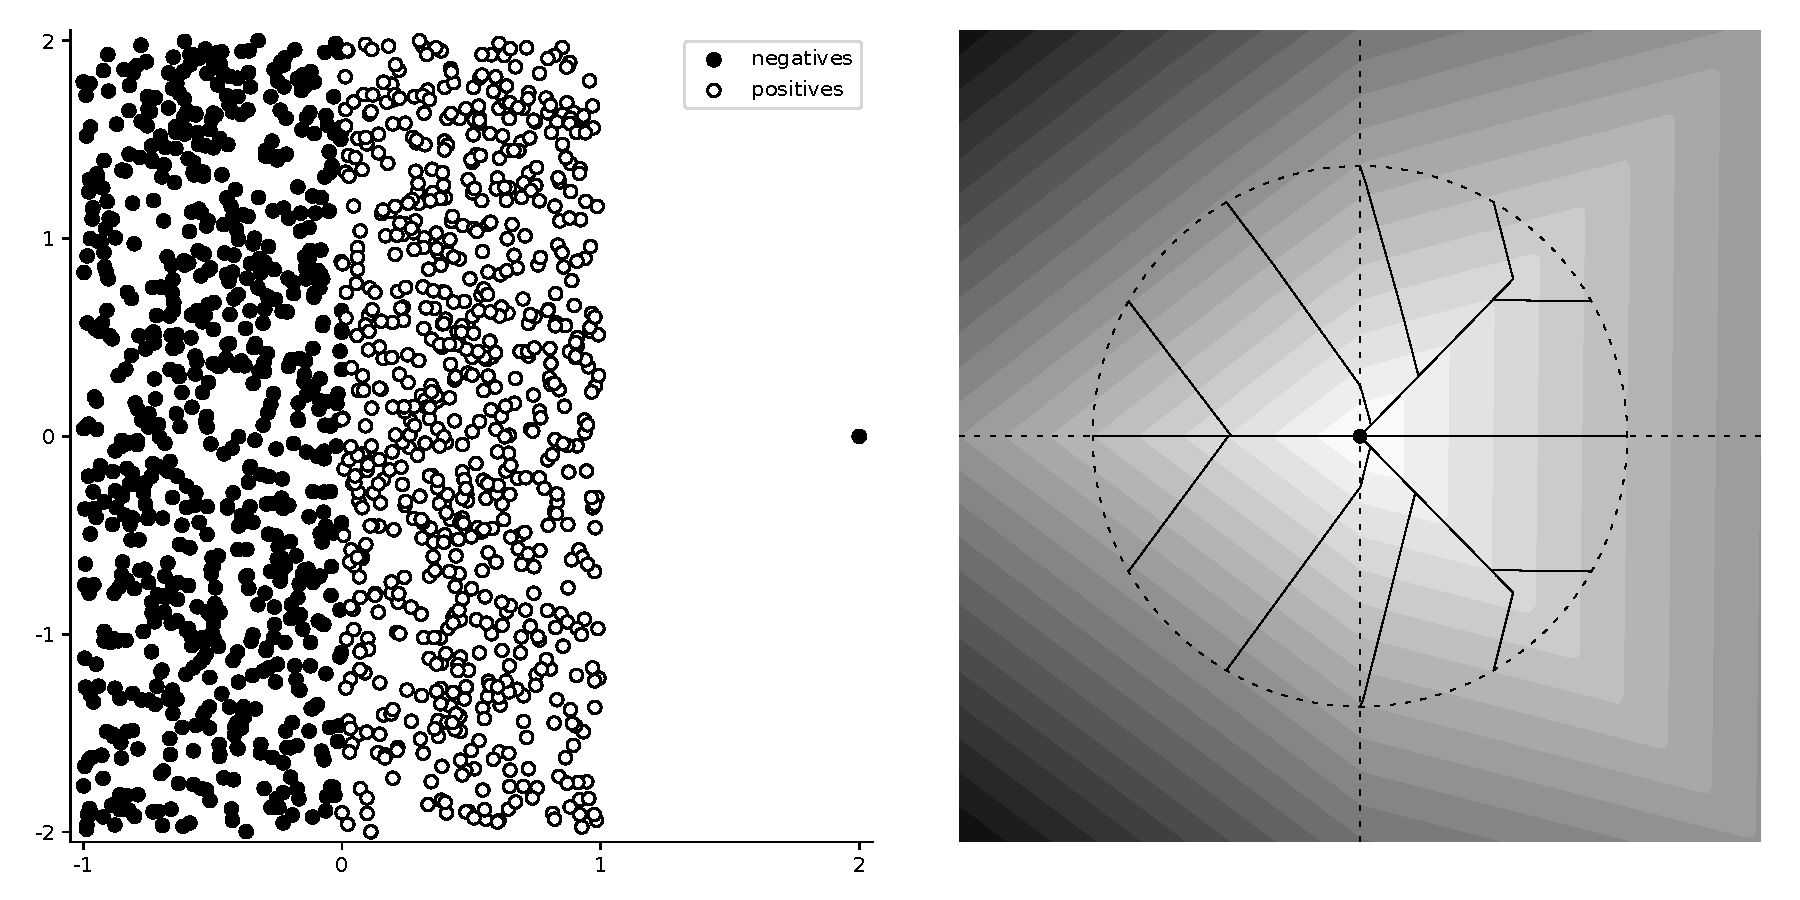
\includegraphics[width=0.7\linewidth]{data/toppush_convergence.pdf}
  \caption{Left: distribution of positive (empty circle) and negative samples (full circles) for the example from Section \ref{sec:example}. Right: contour plot for \TopPush and its convergence to the zero vector from $12$ initial points.}
  \label{fig:example}
\end{figure}

Table \ref{tab:example} shows the threshold $t$ and the objective value $f$ for two points $\bm{w}_1=(0,0)$ and $\bm{w}_2=(1,0)$. These two points are both important: $\bm{w}_1$ does not generate any separating hyperplane, while $\bm{w}_2$ generates the optimal separating hyperplane. We show the precise computation in Appendix \ref{app:example}. Since the dataset is perfectly separable by $\bm{w}_2$, we expect that $\bm{w}_2$ provides a lower objective than $\bm{w}_1$. By shading the better objective in Table~\ref{tab:example} by grey, we see that this did not happen for \TopPush and \TopMeanK.

\begin{table}[!ht]
  \caption{Comparison of formulations on the very simple problem from Section \ref{sec:example}. Two formulations have the global minimum (denoted by grey color) at $\bm{w}_1=(0,0)$ which does not generate any separating hyperplane. The optimal separating hyperplane is generated by $\bm{w}_2=(1,0)$.}
  \label{tab:example}
  \centering
  \begin{tabular}{@{}l ccccc@{}}\toprule
    & & \multicolumn{2}{c}{$\bm{w}_1=(0,0)$} & \multicolumn{2}{c}{$\bm{w}_2=(1,0)$} \\ \cmidrule(lr){3-4} \cmidrule(lr){5-6}
    Name & Label & $t$& $f$ & $t$ & $f$ \\
    \midrule
    \TopPush & \eqref{eq:problem_toppush} & $0$ & \cellcolor{gray!40}$1$ & $2$ & $2.5$ \\
    \TopPushK & \eqref{eq:problem_toppushk} & $0$ & $1$ & $\frac2k$ & \cellcolor{gray!40}$0.5+\frac2k$ \\
    \Grill & \eqref{eq:problem_grill} & $0$ & $2$ & $1-2\tau$ & \cellcolor{gray!40}$1.5+2\tau(1-\tau)$ \\
    \TopMeanK & \eqref{eq:problem_topmeank} & $0$ & \cellcolor{gray!40}$1$ & $1-\tau$ & $1.5-\tau$ \\
    \PatMat & \eqref{eq:problem_patmat}  & $\frac{1}{\beta}(1-\tau)$ & $1+\frac{1}{\beta}(1-\tau)$ & $\frac{1}{\beta}(1-\tau)$ & \cellcolor{gray!40}$0.5+\frac{1}{\beta}(1-\tau)$ \\
    \bottomrule
  \end{tabular}
\end{table}

It can be shown that $\bm{w}_1=(0,0)$ is even the global minimum for \TopPush and \TopMeanK. This raises the question of whether some tricks, such as early stopping or excluding a small ball around zero, cannot overcome this difficulty. The answer is negative as shown in Figure \ref{fig:example} (right). Here, we run \TopPush from several starting points, and it always converges to zero from one of the three possible directions; all of them far from the normal vector to the separating hyperplane.

\subsubsection{Stability and Global minimum at zero}\label{sec:w_zero}

The convexity derived in the previous section guarantees that there are no local minima. However, as we showed in the example above, the global minimum may be at $\bm{w} = \bm{0}$. This is highly undesirable since $\bm{w}$ is the normal vector to the separating hyperplane and the zero vector provides no information. In this section, we analyze when this situation happens. The first result states that if the threshold $t(\bm{w})$ is above a certain value, then zero has a better objective that $\bm{w}$. If this happens for all $\bm{w}$, then zero is the global minimum.

\begin{restatable}{theorem}{larget}\label{thm:large_t}
  Consider any of these formulations: \TopPush, \TopPushK, \TopMeanK or \tauFPL. Fix any $\bm{w}$ and denote the corresponding threshold $t(\bm{w})$. If we have
  \begin{equation*}
    t(\bm{w})\ge \frac{1}{n^+} \sum_{\bm{x}^+ \in \Xc^+} \bm{w}^\top \bm{x}^+,
  \end{equation*}
  then $f(\bm{0})\le f(\bm{w})$. Specifically, denote the scores $s^+=\bm{w}^\top \bm{x}^+$ for $\bm{x}^+\in \Xc^+$ and $s^-=\bm{w}^\top \bm{x}^-$ for $\bm{x}^-\in \Xc^-$ and the ordered variants with decreasing components of $\bm{s}^-$ by $\bm{s}_{[\cdot]}^-$. Then
  \begin{equation}\label{eq:w_zero}
    \begin{aligned}
    s_{[1]}^- \ge \frac{1}{n^+} \sum_{i=1}^{n^+} s_{i}^+
    & \implies f(\bm{0}) \le f(\bm{w}) \text{ for } \TopPush, \\
    \frac{1}{k}\sum_{i=1}^k s_{[i]}^- \ge \frac{1}{n^+} \sum_{i=1}^{n^+} s_{i}^+
    & \implies f(\bm{0})\le f(\bm{w}) \text{ for } \TopPushK, \\
    \frac{1}{n^-\tau} \sum_{i=1}^{n^-\tau} s_{[i]}^- \ge \frac{1}{n^+}\sum_{i=1}^{n^+} s_{i}^+
    & \implies f(\bm{0}) \le f(\bm{w}) \text{ for } \tauFPL. \\
    \end{aligned}
  \end{equation}
\end{restatable}

We can use this result immediately to deduce that some formulations have the global minimum at $\bm{w} = \bm{0}$. More specifically, \TopPush fails if there are outliers, and \TopMeanK fails whenever there are many positive samples.

\begin{corollary}\label{cor:toppush}
  Consider the \TopPush formulation. If the positive samples lie in the convex hull of negative samples, then $\bm{w}=\bm{0}$ is the global minimum.
\end{corollary}

\begin{corollary}\label{cor:topmean}
  Consider the \TopMeanK formulation. If $n^+\ge n\tau$, then $\bm{w}=\bm{0}$ is the global minimum.
\end{corollary}

The proof of Theorem \ref{thm:large_t} employs the fact that all formulations in the theorem statement have only false-negatives in the objective. If $\bm{w}_0=\bm{0}$, then $\bm{w}_0^\top \bm{x}=0$ for all samples $\bm{x}$, the threshold equals to $t=0$ and the objective equals to one. If the threshold is large for $\bm{w}$, many positives are below the threshold, and the false-negatives have the average surrogate value larger than one. In such a case, $\bm{w}_0=\bm{0}$ becomes the global minimum. There are two fixes to this situation:
\begin{itemize}
  \item Include false-positives to the objective. This approach is taken by \Grill and \GrillNP and necessarily results in the loss of convexity.  \item Move the threshold away from zero even when all scores $\bm{w}^\top \bm{x}$ are zero. This approach is taken by our formulations \PatMat and \PatMatNP and keeps convexity.
\end{itemize}
The next theorem shows the advantage of the second approach.

\begin{restatable}{theorem}{patmatzero}\label{thm:patmat_zero}
  Consider the \PatMat or \PatMatNP formulation with the hinge surrogate and no regularization. Assume that for some $\bm{w}$ we have
  \begin{equation}\label{eq:patmat_zero}
    \frac{1}{n^+}\sum_{\bm{x}^+ \in \Xc^+}\bm{w}^\top \bm{x}^+ > \frac{1}{n^-}\sum_{\bm{x}^- \in \Xc^-}\bm{w}^\top \bm{x}^-.
  \end{equation}
  Then there is a scaling parameter $\beta_0$ from \eqref{eq:defin_quantile0} such that $f(\bm{w})<f(\bm{0})$ for all $\beta\in(0,\beta_0)$.
\end{restatable}

These theorem shed some light on the behaviour of the formulations. Theorem \ref{thm:large_t} states that the stability of \tauFPL requires
\begin{equation}\label{eq:stability1}
  \frac{1}{n^-\tau}\sum_{i=1}^{n^-\tau}s_{[i]}^- < \frac{1}{n^+}\sum_{i=1}^{n^+} s_{i}^+,
\end{equation}
while Theorem \ref{thm:patmat_zero} states that the stability of \PatMatNP is ensured by
\begin{equation}\label{eq:stability2}
  \frac{1}{n^-}\sum_{i=1}^{n^-}s_{[i]}^- < \frac{1}{n^+}\sum_{i=1}^{n^+} s_{i}^+.
\end{equation}
The right-hand sides of \eqref{eq:stability1} and \eqref{eq:stability2} are the same, while the left-hand side of \eqref{eq:stability2} is always smaller than the left-hand side of \eqref{eq:stability1}. This implies that if \tauFPL is stable, then \PatMatNP is stable as well.

At the same time, there may be a huge difference in the stability of both formulations. Since the scores of positive samples should be above the scores of negative samples, the scores $s$ may be interpreted as performance. Then formula \eqref{eq:stability1} states that if the mean performance of a \emph{small number of the best} negative samples is larger than the average performance of \emph{all} positive samples, then \tauFPL fails. On the other hand, formula \eqref{eq:stability2} states that if the average performance of \emph{all} positive samples is better than the average performance of \emph{all} negative samples, then \PatMatNP is stable. The former may well happen as accuracy at the top is interested in a good performance of only a small number of positive samples.

\subsection{Method comparison}

We provide a summary of the obtained results in Table \ref{tab:methods}. There we give basic characterizations of the formulations such as their definition label, their source, the hyperparameters, whether the formulation is differentiable and convex, and whether it has stability problems with $\bm{w}=\bm{0}$ being the global minimum. 

\begin{table}[!ht]
  \caption{Summary of the formulations from Section \ref{sec:framework}. The table shows their definition label, the source or the source they are based on, the hyperparameters, whether the formulation is differentiable, convex and stable (in the sense of having problems with $\bm{w}=\bm{0}$).}
  \label{tab:methods}
  \centering
  \begin{tabular}{ll ccccc}\toprule
    Name & Source & Definition & Hyperpars & Convex & Differentiable & Stable \\
    \midrule
    \TopPush & \cite{Li_TopPush} & \eqref{eq:problem_toppush}& $\lambda$ & \yesmark & \nomark & \nomark\\
    \TopPushK & ours & \eqref{eq:problem_toppushk} & $\lambda$, $k$ & \yesmark & \nomark & \nomark\\ 
    \Grill & \cite{Grill_2016} & \eqref{eq:problem_grill}  & $\lambda$ & \nomark & \nomark & \yesmark\\
    \PatMat & ours & \eqref{eq:problem_patmat} & $\beta$, $\lambda$ & \yesmark & \yesmark & \yesmark\\ 
    \TopMeanK & - & \eqref{eq:problem_topmeank} & $\lambda$ & \yesmark & \nomark & \nomark\\ 
    \GrillNP & - & \eqref{eq:problem_grill_np} & $\lambda$ & \nomark & \nomark & \yesmark\\
    \PatMatNP & ours & \eqref{eq:problem_patmat_np} & $\beta$, $\lambda$ & \yesmark & \yesmark & \yesmark\\
    \tauFPL & \cite{zhang2018tau} & \eqref{eq:problem_topmeank_np} & $\lambda$ & \yesmark & \nomark & \nomark\\
    \bottomrule
  \end{tabular}
\end{table}

A similar comparison is performed in Figure \ref{fig:thresholds}. Methods in green and grey are convex, while formulations in white are non-convex. Based on Theorem \ref{thm:large_t}, four formulations in grey are vulnerable to have the global minimum at $\bm{w}=0$. This theorem states that the higher the threshold, the more vulnerable the formulation is. The full arrows depict this dependence. If it points from one formulation to another, the latter one has a smaller threshold and thus is less vulnerable to this undesired global minima. The dotted arrows indicate that this holds usually but not always, the precise formulation is provided in Appendix \ref{app:relations}. This complies with Corollaries \ref{cor:toppush} and \ref{cor:topmean} which state that \TopPush and \TopMeanK are most vulnerable. At the same time, it says that \tauFPL is the best one from the grey-coloured formulations. Finally, even though \PatMatNP has a worse approximation of the true threshold than \tauFPL due to Theorem \ref{thm:large_t}, it is more stable due to the discussion after Theorem \ref{thm:patmat_zero}.

\begin{figure}[!ht]
  \centering
  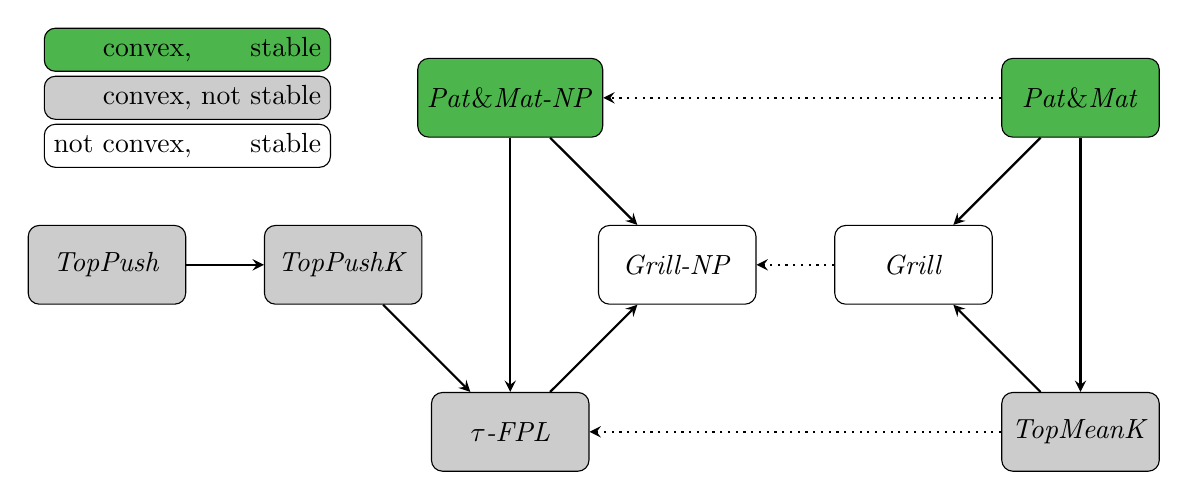
\begin{tikzpicture}[node distance=3cm]
  \node (tikz1) [bubbleB] {\TopPush};
  \node (tikz2) [bubbleB, right of=tikz1] {\TopPushK};
  \node (tikz3) [bubbleA, above right of=tikz2] {\PatMatNP};
  \node (tikz4) [bubbleB, below right of=tikz2] {\tauFPL};
  \node (tikz5) [bubbleC, below right of=tikz3] {\GrillNP};
  \draw [arrowA] (tikz1) -- (tikz2);
  \draw [arrowA] (tikz2) -- (tikz4);
  \draw [arrowA] (tikz3) -- (tikz5);
  \draw [arrowA] (tikz4) -- (tikz5);
  \draw [arrowA] (tikz3) -- (tikz4);
  %
  \node (tikz8) [bubbleC, right of=tikz5] {\Grill};
  \node (tikz6) [bubbleA, above right of=tikz8] {\PatMat};
  \node (tikz7) [bubbleB, below right of=tikz8] {\TopMeanK};
  \draw [arrowA] (tikz6) -- (tikz8);
  \draw [arrowA] (tikz7) -- (tikz8);
  \draw [arrowA] (tikz6) -- (tikz7);
  %
  \draw [arrowB] (tikz6) -- (tikz3);
  \draw [arrowB] (tikz7) -- (tikz4);
  \draw [arrowB] (tikz8) -- (tikz5);
  %
  \node (comm2) [bubbleB, minimum height=3mm, node distance=4.1cm, left of=tikz3] {\phantom{not }convex, not stable};
  \node (comm1) [bubbleA, minimum height=3mm, node distance=6.1mm, above of=comm2] {\phantom{not }convex, \phantom{not }stable};
  \node (comm3) [bubbleC, minimum height=3mm, node distance=6.1mm, below of=comm2] {not convex, \phantom{not }stable};
  \end{tikzpicture}
  \caption{Summary of the formulations from Section \ref{sec:framework}. Methods in green and grey are convex, while formulations in white are non-convex. Methods in grey are vulnerable to have the global minimum at $\bm{w}=0$. Full (dotted) arrow pointing from one formulation to another show that the latter formulation has always (usually) smaller threshold.}
  \label{fig:thresholds}
\end{figure}

\section{Convergence of stochastic gradient descent}\label{sec:convergence}

The previous section analyzed the formulations from Section \ref{sec:framework} but did not consider any optimization algorithms. In this section, we show a basic version of the stochastic gradient descent and then show its convergent version. Since due to considering the threshold, gradient computed on a minibatch is a biased estimate of the true gradient, we need to use variance reduction techniques, and the proof is rather complex.

\subsection{Stochastic gradient descent: Basic}

Many optimization algorithms for solving the formulations from Section \ref{sec:framework} use primal-dual or purely dual formulations. \cite{Eban_2017} introduced dual variables and used alternating optimization to the resulting min-max problem.  \cite{Li_TopPush} and \cite{zhang2018tau} dualized the problem and solved it with the steepest gradient ascent. \cite{macha2020nonlinear} followed the same path but added kernels to handle non-linearity. We follow the ideas of \cite{mackey2018constrained} and \cite{adam2019machine} and solve the problems directly in their primal formulations. Therefore, even though we use the same formulation for \TopPush as \cite{Li_TopPush} or for \tauFPL as \cite{zhang2018tau}, our solution process is different. However, due to convexity, both algorithms should converge to the same point.

The decision variables in \eqref{eq:problem2} are the normal vector of the separating hyperplane $\bm{w}$ and the threshold $t$. To apply an efficient optimization method, we need to compute gradients. The simplest idea \cite{Grill_2016} is to compute the gradient only with respect to $\bm{w}$ and then recompute $t$. A more sophisticated way is based on the chain rule. For each $\bm{w}$, the threshold $t$ can be computed uniquely. We stress this dependence by writing $t(\bm{w})$ instead of $t$. By doing so, we effectively remove the threshold $t$ from the decision variables and $\bm{w}$ remains the only decision variable. Note that the convexity is preserved. Then we can compute the derivative via the chain rule
\begin{equation}\label{eq:derivatives}
  \begin{aligned}
  f(\bm{w}) & = \frac{1}{n^+}\sum_{\bm{x} \in \Xc^+} l(t(\bm{w}) - \bm{w}^\top \bm{x}) + \frac{\lambda}{2}\norm{\bm{w}}^2, \\
  \nabla f(\bm{w}) & = \frac{1}{n^+}\sum_{\bm{x} \in \Xc^+} l'(t(\bm{w}) - \bm{w}^\top \bm{x})(\nabla t(\bm{w}) - \bm{x}) + \lambda \bm{w}.
  \end{aligned}
\end{equation}
The only remaining part is the computation of $\nabla t(\bm{w})$. It is simple for $\nabla t_1(\bm{w})$ and $\nabla t_2(\bm{w})$ and Theorem \ref{thm:derivative} shows the computation for $\nabla t_3(\bm{w})$. Appendix \ref{app:threshold} provides an efficient computation method for $t_3(\bm{w})$.

Having derivative \eqref{eq:derivatives}, deriving the stochastic gradient is simple. It partitions the dataset into minibatches and provides an update of the weights $\bm{w}$ based only on a minibatch, namely by replacing the mean over the whole dataset in \eqref{eq:derivatives} by a mean over the minibatch.

\subsection{Stochastic gradient descent: Convergent for \PatMat and \PatMatNP}

For the convergence proof, we need differentiability which is due to Theorem \ref{thm:derivative} possessed only by \PatMat and \PatMatNP. Therefore, we consider only these two formulations and for simplicity, show it only for \PatMat. We apply a variance reduction technique based on delayed values similar to SAG \cite{schmidt2017minimizing}. 

At iteration $k$ we have the decision variable $\bm{w}^k$ and the active minibatch $I^k$. First, we update the score vector $\bm{s}^k$ only on the active minibatch by setting
\begin{equation}\label{eq:defin_z}
  s_i^k = \begin{cases} \bm{x}_i^\top \bm{w}^k &\text{for all }i\in I^k,\\ s_i^{k-1} &\text{for all }i\notin I^k.\end{cases} 
\end{equation}
We keep scores from previous minibatches intact. We use Appendix \ref{app:threshold} to compute the surrogate quantile $t^k$ as the unique solution of
\begin{equation}\label{eq:update_t}
  \sum_{i \in X}l(\beta(s_i^k - t^k)) = n\tau.
\end{equation}
This is an approximation of the surrogate quantile $t(\bm{w}^k)$ from \eqref{eq:defin_quantile0}. The only difference from the true value $t(\bm{w}^k)$ is that we use delayed scores. Then we introduce artificial variable
\begin{equation}\label{eq:update_a}
  \begin{aligned}
    \bm{a}^k &= \sum_{i\in I^k}l'(\beta(s_i^k - t^k))\bm{x}_i.
  \end{aligned}
\end{equation}
Finally, we approximate the derivative $\nabla f(\bm{w}^k)$ from \eqref{eq:derivatives} by
\begin{equation}\label{eq:update_g}
  g(\bm{w}^k) = \frac{1}{n^k_+}\sum_{i\in I^k_+}l'(t^k - s_i^k)(\nabla t^k - \bm{x}_i),
\end{equation}
where $\nabla t^k$ is an approximation of $\nabla t(\bm{w}^k)$ from Theorem \ref{thm:derivative} defined by
\begin{equation}\label{eq:update_nablat}
  \nabla t^k = \frac{\bm{a}^k + \bm{a}^{k-1} + \dots + \bm{a}^{k - m + 1}}{\sum_{i \in X} l'(\beta(s_i^k - t^k))}.
\end{equation}
A perhaps more straightforward possibility would be to consider only $\bm{a}^k$ in the numerator of \eqref{eq:update_nablat}. However, choice \eqref{eq:update_nablat} enables us to prove the convergence and it adds stability to the algorithm for small minibatches.

The whole procedure does not perform any vector operations outside of the current minibatch~$I^k$. We summarize it in Algorithm \ref{alg:sgd}. Note that a proper initialization for the first $m$ iterations is needed. We finish the theoretical part by the convergence proof.

\begin{algorithm}[!ht]
  \begin{algorithmic}[1]
    \Require Dataset $X$, Minibatches $I^1,\dots,I^m$, Stepsize $\alpha^k$
    \State Initialize weights $\bm{w}^0$
    \For{$k = 0,1,\dots$}
    \State Select a minibatch $I^k$
    \State Compute $s_i^k$ for all $i\in I^k$ according to \eqref{eq:defin_z}
    \State Compute $t^k$ according to \eqref{eq:update_t}
    \State Compute $\bm{a}^k$ according to \eqref{eq:update_a}
    \State Compute $\nabla t^k$ according to \eqref{eq:update_nablat}
    \State Compute $g(\bm{w}^k)$ according to \eqref{eq:update_g}
    \State Set $\bm{w}^{k+1}\gets \bm{w}^k - \alpha^k g(\bm{w}^k)$
    \EndFor
  \end{algorithmic}
  \caption{Stochastic gradient descent for maximizing accuracy at the top}
  \label{alg:sgd}
\end{algorithm}

\begin{restatable}{theorem}{sgd}\label{thm:sgd}
  Consider the \PatMat or \PatMatNP formulation, stepsizes $\alpha^k = \frac{\alpha^0}{k+1}$ and piecewise disjoint minibatches $I^1,\dots,I^m$ which cycle periodically $I^{k+m}=I^k$. If $l$ is the smoothened (Huberized) hinge function, then Algorithm \ref{alg:sgd} converges to the global minimum of \eqref{eq:problem_patmat}.  
\end{restatable}

\section{Numerical experiments}\label{sec:num1}

In this section, we present numerical results.

\subsection{Implementational details and Hyperparameter choice}

We recall that all methods fall into the framework of either \eqref{eq:problem1} or \eqref{eq:problem2}. Since the threshold $t$ depends on the weights $\bm{w}$, we can consider the decision variable to be only $\bm{w}$. Then to apply a method, we implemented the following iterative procedure. At iteration $j$, we have the weights $\bm{w}^j$ to which we compute the threshold $t^j=t(\bm{w}^j)$. Then according to \eqref{eq:derivatives}, we compute the gradient of the objective and apply the ADAM descent scheme \cite{kingma2014adam}. All methods were run for $10000$ iterations using the stochastic gradient descent. The minibatch size was $512$ except for the Ionosphere and Spambase datasets where the full gradient was used. All methods used the hinge surrogate \eqref{eq:defin_surrogate}. The initial point is generated randomly.

We run the methods for the following hyperparameters
\begin{equation}\label{eq:beta1}
  \begin{aligned}
    \beta   & \in  \{0.0001,\ 0.001,\ 0.01,\ 0.1,\ 1,\ 10\}, \\
    \lambda & \in \{0,\ 0.00001,\ 0.0001,\ 0.001,\ 0.01,\ 0.1\}, \\
    k       & \in \{1, 3, 5, 10, 15, 20\}.
  \end{aligned}
\end{equation}
For \TopPushK, \PatMat and \PatMatNP we fixed $\lambda=0.001$ to have six hyperparameters for all methods. For all datasets, we choose the hyperparameter which minimized the criterion on the validation set. The results are computed on the testing set which was not used during training the methods.

\TopPush and \tauFPL were originally implemented in the dual. However, to allow for the same framework and the stochastic gradient descent, we implemented it in the primal. These two approaches are equivalent.

\subsection{Dataset description and Performance criteria}\label{sec:datasets}

For the numerical results, we considered 10 datasets summarized in Table \ref{tab:counts}. They can be downloaded from the UCI repository. Ionosphere \cite{ionosphere} and Spambase are small, Hepmass \cite{hepmass} contains a large number of samples while Gisette \cite{gisette} contains a large number of features. We also considered six visual recognition datasets: MNIST, FashionMNIST, CIFAR10, CIFAR20, CIFAR100 and SVHN2. MNIST and FashionMNIST are grayscale datasets of digits and fashion items, respectively. CIFAR100 is a dataset of coloured images of items grouped into 100 classes. CIFAR10 and CIFAR20 merge these classes into 10 and 20 superclasses, respectively. SVHN2 contains coloured images of house numbers. As Table \ref{tab:counts} shows, these datasets are imbalanced.

Each of the visual recognition datasets was converted into ten binary datasets by considering one of the classes $\{0,\dots,9\}$ as the positive class and the rest as the negative class. The experiments were repeated ten times for each dataset from different seeds, which influenced the starting point and minibatch creation. We use tpr@fpr as the evaluation criterion. This describes the true-positive rate at a prescribed true-negative rate, usually of $1\%$ or $5\%$. For the linear classifier $\bm{w}^\top \bm{x} - t$, it selects the threshold $t$ so that the desired true-negative rate is satisfied and then computes the true-positive rate for this threshold.

\begin{table}[!ht]
  \caption{Structure of the used datasets. The training, validation and testing sets show the number of features $m$, samples $n$ and the fraction of positive samples $\frac{n^+}{n}$.}
  \label{tab:counts}
  \centering
  \begin{tabular}{@{}lllllllll@{}}
    \toprule
    &  & \multicolumn{2}{c}{Training} & \multicolumn{2}{c}{Validation} & \multicolumn{2}{c}{Testing} \\ \cmidrule(lr){3-4} \cmidrule(lr){5-6} \cmidrule(l){7-8} 
    & $m$ & $n$ & $\frac{n^+}{n}$ & $n$ & $\frac{n^+}{n}$ & $n$ & $\frac{n^+}{n}$ \\ \midrule
    Ionosphere
      & $34$
      & $175$ & $36.0\%$ & $88$ & $36.4\%$ & $88$ & $35.2\%$ \\
    Spambase
      & $57$
      & $2300$ & $39.4\%$ & $1150$ & $39.4\%$ & $1151$ & $39.4\%$ \\
    Gisette
      & $5000$
      & $1000$ & $50.0\%$ & $1500$ & $50.0\%$ & $500$ & $50.0\%$ \\
    Hepmass
      & $28$
      & $5250000$ & $50.0\%$ & $1750000$ & $50.0\%$ & $3500000$ & $50.0\%$ \\
    MNIST
      & $28 \times 28 \times 1$
      & $44999$ & $11.2\%$ & $15001$ & $11.2\%$ & $10000$ & $11.4\%$ \\
    FashionMNIST
      & $28 \times 28\times 1$
      & $45000$ & $10.0\%$ & $15000$ & $10.0\%$ & $10000$ & $10.0\%$ \\
    CIFAR10
      & $32\times 32\times 3$
      & $37500$ & $10.0\%$ & $12500$ & $10.0\%$ & $10000$ & $10.0\%$ \\
    CIFAR20
      & $32 \times 32\times 3$
      & $37500$ & $5.0\%$ & $12500$ & $5.0\%$ & $10000$ & $5.0\%$ \\
    CIFAR100
      & $32 \times 32\times 3$
      & $37500$ & $1.0\%$ & $12500$ & $1.0\%$ & $10000$ & $1.0\%$ \\
    SVHN2
      & $32 \times 32\times 3$
      & $54944$ & $18.9\%$ & $18313$ & $18.9\%$ & $26032$ & $19.6\%$ \\
    \bottomrule
  \end{tabular}
\end{table}

\subsection{Numerical results}

Figure \ref{fig:ptau} presents the standard ROC (receiver operating characteristic) curves on selected datasets. Since all methods from this paper are supposed to work at low false-positive rates, the $x$ axis is logarithmic. Both figures depict averages over ten runs with different seeds. The left column depicts CIFAR100 while the right one Hepmass. These are the two more complicated datasets. We selected four representative methods: \PatMat and \PatMatNP as our methods and \TopPush and \tauFPL as state-of-the-art methods. Even though all methods work well, \PatMatNP seems to outperform the remaining methods on most levels of false-positive rate.

\begin{figure}[!ht]
  \centering
  \begin{tikzpicture}
    \pgfplotsset{
      xlabel={False negative rate},
      ylabel={True positive rate},
      xmin = 0.0001,
      xmax = 1,
      xmode = log,
      ymin = -0.05,
      ymax = 1.05,
      ytick = {0,0.2,0.4,0.6,0.8,1},
      grid=major,
      grid style={dashed, gray!50},
      axis x line*=bottom,
    }
    \begin{groupplot}[
        group style = {group size = 2 by 1, horizontal sep = 20pt},
      ]
      \nextgroupplot[
        legend to name={Leg},
        legend style={legend columns=4, column sep = 10pt},
      ]
      \addplot [LinePatMatNP] table[x index=12, y index=13] {\DataCIFAR};
      \addlegendentry{\PatMatNP}
      \addplot [LineTopPush] table[x index=20, y index=21] {\DataCIFAR};
      \addlegendentry{\TopPush}
      \addplot [LinePatMat] table[x index=8, y index=9] {\DataCIFAR};
      \addlegendentry{\PatMat}
      \addplot [LinetauFPL] table[x index=24, y index=25] {\DataCIFAR};
      \addlegendentry{\tauFPL}

      \nextgroupplot[ylabel = {}, yticklabels={}]
      \addplot [LinePatMatNP] table[x index=12, y index=13] {\DataHEPMASS};
      \addplot [LineTopPush] table[x index=20, y index=21] {\DataHEPMASS};
      \addplot [LinePatMat] table[x index=8, y index=9] {\DataHEPMASS};
      \addplot [LinetauFPL] table[x index=24, y index=25] {\DataHEPMASS};
    \end{groupplot}
    \path (group c1r1.north east) -- node[above]{\ref{Leg}} (group c2r1.north west);
  \end{tikzpicture}
  \caption{ROC curves (with logarithmic $x$ axis) on CIFAR100 (left) and Hepmass (right).}
  \label{fig:ptau}
\end{figure}

While Figure \ref{fig:ptau} gave a glimpse of the behaviour of methods, Figures \ref{fig:cd1} and~\ref{fig:cd2} provide a statistically more sound comparison. It employs the Nemenyi post hoc test for the Friedman test recommended in \cite{demvsar2006statistical}. This test compares if the mean ranks of multiple methods are significantly different.

We consider 14 methods (we count different values of $\tau$ as different methods) as depicted in this table. For each dataset mentioned in Section \ref{sec:datasets} and each method, we evaluated the fpr@tpr metric and ranked all methods. Rank 1 refers to the best performance for given criteria, while rank 14 is the worst. The $x$-axis shows the average rank over all datasets. The Nemenyi test computes the critical difference. If two methods are within their critical difference, their performance is not deemed to be significantly different. Black wide horizontal lines group such methods.

\begin{figure}[!ht]
    \centering
    \resizebox{\linewidth}{!}{
  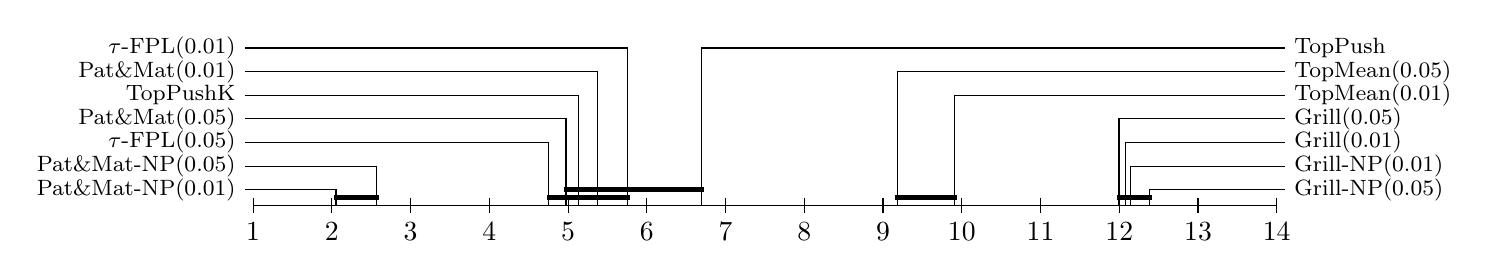
\begin{tikzpicture}[scale = 1.0]
    \draw (1.0,0) -- (14.0,0);
    \foreach \x in {1,...,14} \draw (\x,0.10) -- (\x,-0.10) node[anchor=north]{$\x$};
    \draw (2.051948051948052,0) -- (2.051948051948052,0.19999999999999998) -- (0.9, 0.19999999999999998) node[anchor=east] {\footnotesize Pat\&Mat-NP(0.01)};
    \draw (2.564935064935065,0) -- (2.564935064935065,0.5) -- (0.9, 0.5) node[anchor=east] {\footnotesize Pat\&Mat-NP(0.05)};
    \draw (4.7564935064935066,0) -- (4.7564935064935066,0.7999999999999999) -- (0.9, 0.7999999999999999) node[anchor=east] {\footnotesize $\tau$-FPL(0.05)};
    \draw (4.974025974025974,0) -- (4.974025974025974,1.0999999999999999) -- (0.9, 1.0999999999999999) node[anchor=east] {\footnotesize Pat\&Mat(0.05)};
    \draw (5.136363636363637,0) -- (5.136363636363637,1.4) -- (0.9, 1.4) node[anchor=east] {\footnotesize TopPushK};
    \draw (5.37012987012987,0) -- (5.37012987012987,1.6999999999999997) -- (0.9, 1.6999999999999997) node[anchor=east] {\footnotesize Pat\&Mat(0.01)};
    \draw (5.753246753246753,0) -- (5.753246753246753,2.0) -- (0.9, 2.0) node[anchor=east] {\footnotesize $\tau$-FPL(0.01)};
    \draw (6.694805194805195,0) -- (6.694805194805195,1.9999999999999998) -- (14.1, 1.9999999999999998) node[anchor=west] {\footnotesize TopPush};
    \draw (9.181818181818182,0) -- (9.181818181818182,1.7) -- (14.1, 1.7) node[anchor=west] {\footnotesize TopMean(0.05)};
    \draw (9.905844155844155,0) -- (9.905844155844155,1.4) -- (14.1, 1.4) node[anchor=west] {\footnotesize TopMean(0.01)};
    \draw (11.996753246753247,0) -- (11.996753246753247,1.0999999999999999) -- (14.1, 1.0999999999999999) node[anchor=west] {\footnotesize Grill(0.05)};
    \draw (12.084415584415584,0) -- (12.084415584415584,0.8) -- (14.1, 0.8) node[anchor=west] {\footnotesize Grill(0.01)};
    \draw (12.146103896103897,0) -- (12.146103896103897,0.5) -- (14.1, 0.5) node[anchor=west] {\footnotesize Grill-NP(0.01)};
    \draw (12.383116883116884,0) -- (12.383116883116884,0.2) -- (14.1, 0.2) node[anchor=west] {\footnotesize Grill-NP(0.05)};
    \draw[line width=0.06cm,color=black,draw opacity=1.0] (2.021948051948052,0.1) -- (2.594935064935065,0.1);
    \draw[line width=0.06cm,color=black,draw opacity=1.0] (4.726493506493506,0.1) -- (5.783246753246753,0.1);
    \draw[line width=0.06cm,color=black,draw opacity=1.0] (4.9440259740259735,0.2) -- (6.724805194805195,0.2);
    \draw[line width=0.06cm,color=black,draw opacity=1.0] (9.151818181818182,0.1) -- (9.935844155844155,0.1);
    \draw[line width=0.06cm,color=black,draw opacity=1.0] (11.966753246753248,0.1) -- (12.413116883116883,0.1);
  \end{tikzpicture}
}

    \caption{Critical difference (CD) diagrams (level of importance 0.05) of the Nemenyi post hoc test for the Friedman test. Each diagram shows the mean rank of each method, with rank 1 being the best. Black wide horizontal lines group together methods with the mean ranks that are not significantly different. The critical difference diagrams were computed for mean rank averages over all datasets of the tpr@fpr ($\tau=0.01$) metric.}
    \label{fig:cd1}
\end{figure}

\begin{figure}[!ht]
    \centering
    \resizebox{\linewidth}{!}{
  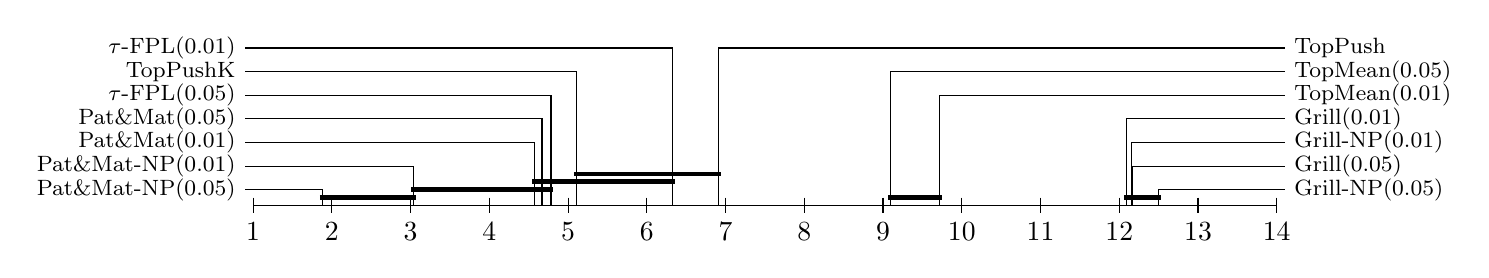
\begin{tikzpicture}[scale = 1.0]
    \draw (1.0,0) -- (14.0,0);
    \foreach \x in {1,...,14} \draw (\x,0.10) -- (\x,-0.10) node[anchor=north]{$\x$};   \draw (1.8766233766233766,0) -- (1.8766233766233766,0.19999999999999998) -- (0.9, 0.19999999999999998) node[anchor=east] {\footnotesize Pat\&Mat-NP(0.05)};
    \draw (3.0357142857142856,0) -- (3.0357142857142856,0.5) -- (0.9, 0.5) node[anchor=east] {\footnotesize Pat\&Mat-NP(0.01)};
    \draw (4.577922077922078,0) -- (4.577922077922078,0.7999999999999999) -- (0.9, 0.7999999999999999) node[anchor=east] {\footnotesize Pat\&Mat(0.01)};
    \draw (4.6688311688311686,0) -- (4.6688311688311686,1.0999999999999999) -- (0.9, 1.0999999999999999) node[anchor=east] {\footnotesize Pat\&Mat(0.05)};
    \draw (4.782467532467533,0) -- (4.782467532467533,1.4) -- (0.9, 1.4) node[anchor=east] {\footnotesize $\tau$-FPL(0.05)};
    \draw (5.103896103896104,0) -- (5.103896103896104,1.6999999999999997) -- (0.9, 1.6999999999999997) node[anchor=east] {\footnotesize TopPushK};
    \draw (6.327922077922078,0) -- (6.327922077922078,2.0) -- (0.9, 2.0) node[anchor=east] {\footnotesize $\tau$-FPL(0.01)};
    \draw (6.9058441558441555,0) -- (6.9058441558441555,1.9999999999999998) -- (14.1, 1.9999999999999998) node[anchor=west] {\footnotesize TopPush};
    \draw (9.097402597402597,0) -- (9.097402597402597,1.7) -- (14.1, 1.7) node[anchor=west] {\footnotesize TopMean(0.05)};
    \draw (9.714285714285714,0) -- (9.714285714285714,1.4) -- (14.1, 1.4) node[anchor=west] {\footnotesize TopMean(0.01)};
    \draw (12.090909090909092,0) -- (12.090909090909092,1.0999999999999999) -- (14.1, 1.0999999999999999) node[anchor=west] {\footnotesize Grill(0.01)};
    \draw (12.152597402597403,0) -- (12.152597402597403,0.8) -- (14.1, 0.8) node[anchor=west] {\footnotesize Grill-NP(0.01)};
    \draw (12.162337662337663,0) -- (12.162337662337663,0.5) -- (14.1, 0.5) node[anchor=west] {\footnotesize Grill(0.05)};
    \draw (12.503246753246753,0) -- (12.503246753246753,0.2) -- (14.1, 0.2) node[anchor=west] {\footnotesize Grill-NP(0.05)};
    \draw[line width=0.06cm,color=black,draw opacity=1.0] (1.8466233766233766,0.1) -- (3.0657142857142854,0.1);
    \draw[line width=0.06cm,color=black,draw opacity=1.0] (3.005714285714286,0.2) -- (4.812467532467533,0.2);
    \draw[line width=0.06cm,color=black,draw opacity=1.0] (4.5479220779220775,0.30000000000000004) -- (6.357922077922078,0.30000000000000004);
    \draw[line width=0.06cm,color=black,draw opacity=1.0] (5.073896103896104,0.4) -- (6.935844155844156,0.4);
    \draw[line width=0.06cm,color=black,draw opacity=1.0] (9.067402597402598,0.1) -- (9.744285714285713,0.1);
    \draw[line width=0.06cm,color=black,draw opacity=1.0] (12.060909090909092,0.1) -- (12.533246753246752,0.1);
  \end{tikzpicture}
}

    \caption{Critical difference (CD) diagrams (level of importance 0.05) of the Nemenyi post hoc test for the Friedman test. Each diagram shows the mean rank of each method, with rank 1 being the best. Black wide horizontal lines group together methods with the mean ranks that are not significantly different. The critical difference diagrams were computed for mean rank averages over all datasets of the tpr@fpr ($\tau=0.05$) metric.}
    \label{fig:cd2}
\end{figure}

From this figure and table, we make several observations:
\begin{itemize}
  \item \TopPushK (rank 5.1) provides a slight improvement over \TopPush (rank 6.7) even though this improvement is not statistically significant as both methods are connected by the black line in both Figures \ref{fig:cd1} and \ref{fig:cd2}.
  \item Neither \Grill (ranks 12.0 and 12.1) nor \GrillNP (ranks 12.1 and 12.4) perform well. We believe this happened due to the lack of convexity as indicated in Theorem \ref{thm:convex} and the discussion after that.
  \item \TopMeanK (ranks 9.2 and 9.9) does not perform well either. Since the thresholds $\tau$ are small, then $\bm{w}=0$ is the global minimum as proved in Corollary \ref{cor:topmean}.
  \item \PatMatNP (rank 2.1 and 2.6) seems to outperform other methods.
  \item \PatMat (ranks 5.0 and 5.4), \tauFPL (ranks 4.8 and 5.8) and \TopPushK (rank 5.1) perform similarly. Since they are connected, there is no statistical difference between their behaviours.
  \item \PatMatNP at level $0.01$ (rank 2.1) outperforms \PatMatNP at level $0.05$ (rank 2.6) for $\tau=0.01$. \PatMatNP at level $0.05$ (rank 1.9 in Figure \ref{fig:cd2}) outperforms \PatMatNP at level $0.01$ (rank 3.0 in Figure \ref{fig:cd2}) for $\tau=0.05$. This should be because these methods are optimized for the corresponding threshold. For $\tauFPL$ we observed this behaviour for Figure \ref{fig:cd2} but not for Figure \ref{fig:cd1}.
\end{itemize}

Figure \ref{fig:wilcoxon} provides a similar comparison. Both axes are sorted from the best (left) to the worst (right) average ranks. The numbers in the graph show the $p$-value for the pairwise Wilcoxon signed-rank test, where the null hypothesis is that the mean tpr@fpr of both methods is the same. Even though Figure \ref{fig:cd1} employs a comparison of mean ranks and Figure \ref{fig:wilcoxon} a pairwise comparison of fpr@tpr, the results are almost similar. Methods grouped by the black line in the former figure usually show a large $p$-value in the latter figure.

\begin{figure}[!ht]
    \centering
    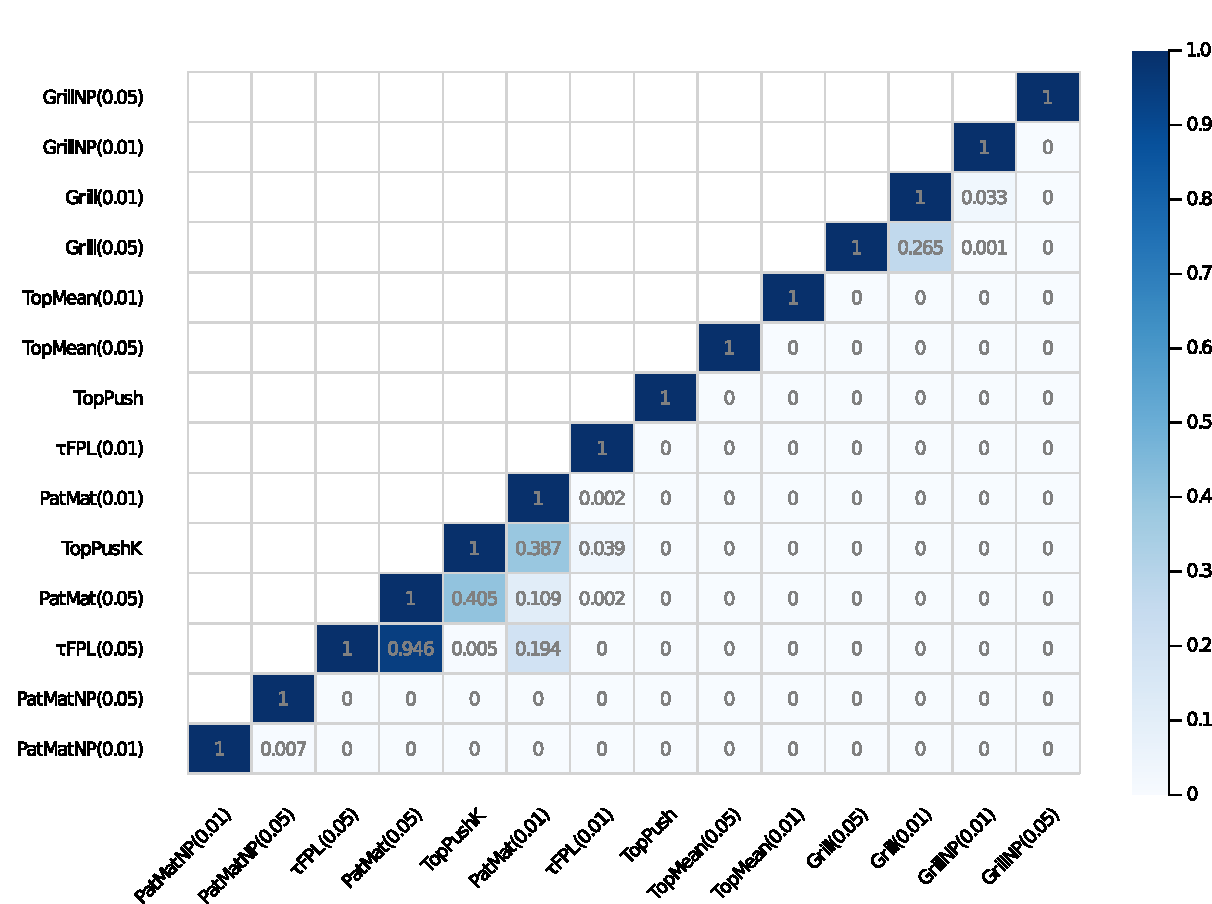
\includegraphics[width = \linewidth]{data/wilcoxon_fpr_1.pdf}
    \caption{The $p$-value for the parwise Wilcoxon signed-rank test, where the null hypothesis is that the mean tpr@fpr(0.01) of both methods is the same. The methods are sorted by mean rank (left = better).}
    \label{fig:wilcoxon}
\end{figure}

Table \ref{tab:fails} investigates the impact of $\bm{w}=0$ as a potential global minimum. Each method was optimized for six different values of hyperparameters. The table depicts the condition under which the final value has a lower objective than $\bm{w}=0$. Thus, \yesmark\ means that it is always better while \nomark\ means that the algorithm made no progress from the starting point $\bm{w} =0$. The latter case implies that $\bm{w}=0$ seems to be the global minimum. We make the following observations:
\begin{itemize}
  \item \PatMat and \PatMatNP are the only methods which succeeded at every dataset for some hyperparameter. Moreover, for each dataset, there was some $\beta_0$ such that these methods were successful if and only if $\beta\in(0,\beta_0)$. This is in agreement with Theorem~\ref{thm:patmat_zero}.
  \item \TopMeanK fails everywhere which agrees with Corollary \ref{cor:topmean}.
  \item Figure \ref{fig:thresholds} states that the methods from Section \ref{sec:obj2} has a higher threshold than their Neyman-Pearson variants from Section \ref{sec:obj3}. This is documented in the table as the latter have a higher number of successes.
\end{itemize}

\begin{table}[!ht]
  \caption{Necessary hyperparameter choice for the solution to have a better objective than zero. \yesmark\ means that the solution was better than zero for all hyperparameters while \nomark\ means that it was worse for all hyperparameters.}
  \label{tab:fails}
  \centering
  \begin{tabular}{@{}lllll@{}}
    \toprule
    & Ionosphere & Hepmass & FashionMNIST & CIFAR100 \\
    \midrule
    \TopPush
      & \yesmark & \nomark & \yesmark & \nomark \\
    \TopPushK
      & \yesmark & \nomark & \yesmark & \nomark \\
    \Grill$\tau=0.01$
      & \nomark & \nomark & \nomark & \nomark \\
    \phantom{\Grill}$\tau=0.05$
      & \nomark &\nomark & \nomark & \nomark \\
    \PatMat$\tau=0.01$
      & \yesmark & \good{\boldmath$\beta\le 0.1$} & \good{\boldmath$\beta\le 1$} & \good{\boldmath$\beta\le 1$} \\
    \phantom{\PatMat}$\tau=0.05$
      & \yesmark & \good{\boldmath$\beta\le 1$} & \yesmark & \yesmark \\
    \TopMeanK$\tau=0.01$
      & \nomark & \nomark & \nomark & \nomark \\
    \phantom{\TopMeanK}$\tau=0.05$
      & \nomark & \nomark & \nomark & \nomark \\
    \GrillNP$\tau=0.01$
      & \nomark & \nomark & \nomark & \nomark \\
    \phantom{\GrillNP}$\tau=0.05$
      & \nomark & \nomark & \nomark & \nomark \\
    \PatMatNP$\tau=0.01$
      & \yesmark & \good{\boldmath$\beta\le 1$} & \yesmark & \good{\boldmath$\beta\le 1$} \\
    \phantom{\PatMatNP}$\tau=0.05$
      & \yesmark & \yesmark & \yesmark & \good{\boldmath$\beta\le 1$} \\
    \tauFPL$\tau=0.01$
      & \yesmark & \nomark & \yesmark & \nomark \\
    \phantom{\tauFPL}$\tau=0.05$
      & \yesmark & \yesmark & \yesmark & \good{\boldmath$\lambda\le 0.001$} \\
    \bottomrule
  \end{tabular}
\end{table}

\section{Conclusion}

In this paper, we achieved the following results:
\begin{itemize}
  \item We presented a unified framework for the three criteria from Section \ref{sec:framework}. These criteria include ranking, accuracy at the top and hypothesis testing.
  \item We showed that several known methods (\TopPush, \Grill, \tauFPL) fall into our framework and derived some completely new methods (\PatMat, \PatMatNP).
  \item We performed a theoretical analysis of the methods. We showed that known methods suffer from certain disadvantages. While \TopPush and \tauFPL are sensitive to outliers, \Grill is non-convex. We proved the global convergence of the stochastic gradient descent for \PatMat and \PatMatNP.
  \item We performed a numerical comparison and we showed a good performance of our method \PatMatNP.
\end{itemize}
\chapter{Non-linear Classification at the Top}

\section{Introduction}
    
The aim of classical linear binary classification is to separate positive and negative samples by a linear hyperplane. In many applications, it is desirable to separate only a certain number of samples. In such a case, the goal is not to maximize the performance on all samples but only the performance on the required samples with the highest relevance. Such classifiers have many applications. For example, in information retrieval systems, only the most relevant documents should be returned for a given query. Furthermore, they are useful in domains, where a large number of samples needs to be quickly screened and only a small subset of samples needs to be selected for further evaluation.

These problems can be generally written as pushing the positive samples above some decision threshold. The methods differ in the definition of the decision threshold. In our previous work~\cite{adam2019patmat}, we introduced a general framework that unifies these methods. We showed that several problem classes, which were considered as separate problems so far, fit into the framework. As the most relevant we mention the following methods:
\begin{itemize}
  \item \emph{Ranking problems} focuses on ranking the positive samples higher than the negative ones. Many methods, such as \emph{RankBoost}~\cite{freund2003efficient}, \emph{Infinite Push}~\cite{agarwal2011infinite} or \emph{$p$-norm push}~\cite{rudin2009pnorm} employ a pairwise comparison of samples, which makes them infeasible for larger datasets. This was alleviated in \TopPush~\cite{li2014top} where the authors considered the limit~$p \rightarrow \infty$. Since the $l_{\infty}$ norm from \TopPush is equal to the maximum, the decision threshold from our framework equals to the maximum of scores of negative samples. This was generalized into \TopPushK~\cite{adam2019patmat} by considering the threshold to be the mean of~$K$ largest scores of negative samples.

  \item \AccatTop~\cite{boyd2012accuracy} focuses on maximizing the number of positive samples above the top $\tau$-quantile of scores. There are many methods on how to solve accuracy at the top. In~\cite{boyd2012accuracy}, the authors assume that the top quantile is one of the samples, construct~$n$ unconstrained optimization problems with fixed thresholds, solve them and select the best solution. This method is computationally expensive. In~\cite{grill2016learning} the authors propose a fast projected gradient descent method. In our previous paper, we proposed a convex approximation of the accuracy at the top called \PatMat. This method is reasonably fast and guaranteed the existence of global optimum.
\end{itemize}

The deficiency of methods from this framework is that they usually cover only linear classifiers. However, as many problems are not linearly separable, nonlinear classifiers are needed. In this work, we show how to extend our framework into nonlinear classification problems. To do so, we use the fact that our framework is similar to the primal formulation of support vector machines~\cite{cortes1995support}. The classical way to incorporate nonlinearity into SVM is to derive the dual formulation~\cite{boyd2004convex} and to employ the kernels method~\cite{scholkopf2001learning}. In this work, we follow this approach, derive dual formulations for the considered problems and add nonlinear kernels to them. Moreover, as dual problems are generally expensive to solve, we derive a quick method to solve them. This is a modification of the coordinate-wise dual ascent from~\cite{hsieh2008dual}. For a review of other approaches see \cite{batmaz2019review,werner2019review}.

The paper is organized as follows: In Section~\ref{sec:Derivation of dual problems} we recall the unified framework derived in~\cite{adam2019patmat} and two class of problems that falls into it. Moreover, for selected methods, we derive their dual formulations. Namely, we focus on \TopPush, \TopPushK and \PatMat. In Section~\ref{sec:New method for solving dual problems}, we show how to add nonlinear kernels into dual formulations, derive a new method for solving these dual problems and perform its complexity analysis. Since our method depends on the chosen problem and surrogate function, we provide a concrete form of the solution for \TopPushK with the truncated quadratic loss. Solutions for other problems are provided in Appendix~\ref{sec:Computing Delta with truncated quadratic surrogate} and~\ref{sec:Computing Delta with hinge surrogate}. Finally, in Section~\ref{sec:Numerical experiments} we present the description of performance criteria, choice of hyperparameters and description of datasets. The rest of the section is focused on the results of numerical experiments. Here we compare all methods in terms of overall accuracy and accuracy at a given threshold. We also discuss the convergence and time consumption of all methods. All our codes are available online.\footnote{\texttt{https://github.com/VaclavMacha/ClassificationOnTop\_nonlinear.jl}}

\section{Derivation of dual problems}\label{sec:Derivation of dual problems}

Linear binary classification is a problem of finding a linear hyperplane that separates a group of positive samples from a group of negative samples and achieves the lowest possible error. For a sample~$\bm{x} \in \R^d,$ the prediction for a linear classifier amounts to
\begin{equation*}
  \bm{x} \textnormal{ has }
  \begin{dcases*}
    \textnormal{positive label} & if~$\bm{w}^{\top} \bm{x} \geq t$, \\
    \textnormal{negative label} & otherwise.
  \end{dcases*}
\end{equation*}
Here,~$\bm{w} \in \R^{d}$ is the normal vector to the separating hyperplane and~$t \in \R$ is a decision threshold. The well-known example of such a classifier is a support vector machine~\cite{cortes1995support} where the decision threshold~$t$ is a free variable. However, many important binary classification problems maximize the performance only for a certain amount of samples with the highest scores~$s = \bm{w}^{\top}\bm{x}.$ In these cases, the threshold~$t$ is not a free variable but a function of the scores. In our previous work~\cite{adam2019patmat}, we formulated a general framework for maximizing performance above the threshold $t$ as
\begin{equation}\label{eq:General problem}
  \begin{aligned}
    \minimize{\bm{w}, t}
    & \frac{1}{2} \norm{\bm{w}}_{2}^{2} + C \sum_{i = 1}^{n^+} [t - \bm{w}^{\top}\bm{x}^+_{i}] \\
    \st
    & \textnormal{threshold} \ t \ \textnormal{is a function of } \{\bm{w}^{\top} \bm{x_i}\}_{i=1}^n,
  \end{aligned}
\end{equation}
where~$C \in \R$ is a constant;~$[\cdot]$ is the $0-1$~loss defined as~$1$ if the argument is true and~$0$ otherwise. To denote positive and negative samples, we use~$+$ and $-$ symbols in the superscript, respectively. Note that $[t - \bm{w}^{\top}\bm{x}^+_{i}]$ counts the number of positive samples $\bm x_i^+$ whose score $\bm{w}^\top \bm x_i^+$ is below the threshold $t$. Since the objective is to be minimized, the positive samples should lie above the threshold $t$.

Since the objective function in~\eqref{eq:General problem} is discontinuous due to the $0-1$~loss, the optimization problem~\eqref{eq:General problem} is difficult. A typical approach to remove this unwanted feature is to approximate the $0-1$~loss by a surrogate function such as the truncated quadratic or the hinge functions
\begin{align}
    l_{\textnormal{quadratic}}(s)
    & = (\max\{0,1 + \vartheta s\})^{2}, \label{eq:Truncated quadratic loss} \\
    l_{\textnormal{hinge}}(s)
    & = \max\{0,1 + \vartheta s\} \label{eq:Hinge loss},
\end{align}
where $\vartheta > 0$ is a scaling parameter. In the following text, we use the symbol~$l$ to denote any convex non-negative non-decreasing function with~$l(0) = 1.$ Replacing the $0-1$~loss in~\eqref{eq:General problem} by a surrogate function results in
\begin{equation}\label{eq:General surrogate problem}
  \begin{aligned}
    \minimize{\bm{w}, t}
    & \frac{1}{2} \norm{\bm{w}}_{2}^{2} + C \sum_{i = 1}^{n^+} l(t - \bm{w}^{\top}\bm{x}^+_{i}) \\
    \st
    & \textnormal{threshold} \ t \ \textnormal{is a function of } \{\bm{w}^{\top} \bm{x_i}\}_{i=1}^n.
  \end{aligned}
\end{equation}
Note that the objective function in~\eqref{eq:General surrogate problem} is continuous.

As we derived in~\cite{adam2019patmat}, there are many problems belonging to the general framework~\eqref{eq:General problem}. However, this framework handles only linear classification problems. As many problems are not linearly separable, this is often not sufficient. To generalize the framework to nonlinear classifiers, we realize that~\eqref{eq:General surrogate problem} is similar to the primal formulation of the SVM~\cite{cortes1995support}. We will follow the standard way to incorporate nonlinearity into SVM by deriving the dual problem~\cite{boyd2004convex} and using the kernels methods~\cite{scholkopf2001learning}.

In the remainder of this section, we recall two problem classes from~\cite{adam2019patmat} and their convex approximations, and for each of them, we derive its dual formulation. Namely, we will discuss \TopPushK and \AccatTop with its convex approximation \PatMat.

\subsection{\TopPushK}

The first problem \TopPushK is our modification of the \TopPush method introduced in~\cite{li2014top}. It selects the threshold $t$ as the mean of the scores corresponding to $K$ highest ranked negatives. By doing so, it enforces the positives to be ranked above negatives. Therefore, both \TopPush ($K=1$) and \TopPushK ($K>1$) fall into the category of ranking problems.

Writing this more formally, define vector~$\bm{s}$ of all scores as~$s_i = \bm{w}^{\top} \bm{x}_i$ for all~$i = 1, 2, \ldots, n$ and its sorted version~$\bm{s}_{[\cdot]}$ with decreasing components, i.e. $s_{[1]} \geq s_{[2]} \geq \cdots  \geq s_{[n]}$. Then \TopPushK reads
\begin{equation}\label{eq:TopPushK primal}
  \begin{aligned}
    \minimize{\bm{w}, t, \bm s^-}
    & \frac{1}{2} \norm{\bm{w}}_{2}^{2} + C \sum_{i = 1}^{n^+} l(t - \bm{w}^{\top}\bm{x}^+_{i}) \\
    \st
    & t = \frac{1}{K}\sum_{j = 1}^{K} s^{-}_{[j]}, \\
    & s_j^- = \bm{w}^\top \bm x_j^-, \quad \forall j = 1, 2, \ldots, n^-.
  \end{aligned}
\end{equation}
It can be showed that this problem is convex and that for~$K = 1$ we get the original \TopPush.

In the following theorem, we denote the positive semidefinite kernel matrix $\K$ by
\begin{equation}\label{eq:kernel_linear}
  \K = \Matrix{\X^+ \\ - \X^-} \Matrix{\X^+ \\ - \X^-}^\top = \Matrix{\X^+ \X^{+\top} & -\X^+ \X^{-\top} \\ -\X^- \X^{+\top} & \X^- \X^{-\top} }.
\end{equation}
and show the form of the \TopPushK dual problem\footnote{To keep the readability of the paper, we postpone all proofs to the Appendix}.

\begin{restatable}[\TopPushK dual formulation]{theorem}{toppushkdual}\label{thm:TopPushK dual}
  The dual problem corresponding to the problem~\eqref{eq:TopPushK primal} has the form
  \begin{subequations}\label{eq:TopPushK dual}
    \begin{alignat}{2}
      \maximize{\bm{\alpha}, \bm{\beta}}
      & - \frac{1}{2} \Matrix{\bm{\alpha} \\ \bm{\beta}}^\top \K \Matrix{\bm{\alpha} \\ \bm{\beta}} - C \sum_{i = 1}^{n^+} l^{\star}\Brac{\frac{\alpha_i}{C}} \span \span \label{eq:TopPushK dual objective} \\
      \st
      & \sum_{i = 1}^{n^+} \alpha_i = \sum_{j = 1}^{n^-} \beta_j, \label{eq:TopPushK dual constraint 1} \\
      & 0 \leq \beta_j \leq \frac{1}{K} \sum_{i = 1}^{n^+} \alpha_i,  && \quad \forall j = 1, 2, \ldots, n^-, \label{eq:TopPushK dual constraint 2}
    \end{alignat}
    where $l^{\star}$ is a conjugate of the surrogate loss function $l$ from~\eqref{eq:TopPushK primal} and $\K$ was defined in~\eqref{eq:kernel_linear}.
  \end{subequations}
\end{restatable}

\subsection{\AccatTop}

The second problem \AccatTop was introduced in~\cite{boyd2012accuracy}. On the contrary to \TopPushK, which focuses on the minimization of the number of positive samples below $K$~highest ranked negatives, the \AccatTop minimizes the number of positive samples below the top $\tau$-quantile from negative samples defined as
\begin{equation}\label{eq:Quantile}
    t = \max \Set{t}{\sum_{j = 1}^{n^-} [\bm{w}^\top \bm{x}_j^- - t] \geq n \tau}.
\end{equation}
Then \AccatTop is an optimization problem written as follows
\begin{equation}\label{eq:AccAtTop}
  \begin{aligned}
    \minimize{\bm{w}, t}
    & \frac{1}{2} \norm{\bm{w}}_{2}^{2} + C \sum_{i = 1}^{n^+} l_1(t - \bm{w}^{\top}\bm{x}^+_{i}) \\
    \st
    & t \ \textnormal{is the surrogate top} \ \tau\textnormal{-quantile: it solves~\eqref{eq:Quantile}}.
  \end{aligned}
\end{equation}
Since it is known that the quantile function~\eqref{eq:Quantile} is non-convex, we derived its convex surrogate approximation
\begin{equation}\label{eq:Surrogate quantile}
  t \quad \textnormal{solves} \quad \sum_{j = 1}^{n^-} l_2(\bm{w}^{\top}\bm{x}_{j}^- - t) \leq n \tau.
\end{equation}
Replacing the true quantile~\eqref{eq:Quantile} by its surrogate approximation~\eqref{eq:Surrogate quantile} yields
\begin{equation}\label{eq:PatMat primal}
  \begin{aligned}
    \minimize{\bm{w}, t}
    & \frac{1}{2} \norm{\bm{w}}_{2}^{2} + C \sum_{i = 1}^{n^+} l_1(t - \bm{w}^{\top}\bm{x}^+_{i}) \\
    \st & t \ \textnormal{is the top} \ \tau\textnormal{-quantile: it solves~\eqref{eq:Surrogate quantile}}.
  \end{aligned}
\end{equation}
In~\cite{adam2019patmat}, we called the convex problem~\eqref{eq:PatMat primal} \PatMat. The following theorem shows its dual form.

\begin{restatable}[\PatMat dual formulation]{theorem}{patmatdual}\label{thm:PatMat dual}
  The dual problem corresponding to the problem~\eqref{eq:PatMat primal} has the form
  \begin{subequations}\label{eq:PatMat dual}
    \begin{align}
      \maximize{\bm{\alpha}, \bm{\beta}, \delta}
      & -\frac{1}{2} \Matrix{\bm{\alpha} \\ \bm{\beta}}^\top \K \Matrix{\bm{\alpha} \\ \bm{\beta}} - C \sum_{i = 1}^{n^+} l_1^{\star} \Brac{\frac{\alpha_i}{C}} - \delta \sum_{j = 1}^{n^-} l_2^{\star} \Brac{\frac{\beta_j}{\delta}} - \delta n \tau \label{eq:PatMat dual objective} \\
      \st
      & \sum_{i = 1}^{n^+} \alpha_i = \sum_{j = 1}^{n^-} \beta_j, \label{eq:PatMat dual constraint 1} \\
      & \delta \geq 0, \label{eq:PatMat dual constraint 2} 
    \end{align}
    where $l_1^{\star}$, $l_2^{\star}$ are conjugates of the surrogate loss functions $l_1,$ $l_2$ from~\eqref{eq:PatMat primal} and $\K$ was defined in~\eqref{eq:kernel_linear}.
  \end{subequations}
\end{restatable}

\section{New method for solving dual problems}\label{sec:New method for solving dual problems}

In the previous section, we derived the dual formulations for the \TopPushK and \PatMat problems. These dual formulations allow us to incorporate nonlinearity using kernels~\cite{scholkopf2001learning} in the same way as in SVM. Since the dimension of~\eqref{eq:TopPushK dual} and~\eqref{eq:PatMat dual} equals to the number of samples $n$, it is computationally expensive to use standard techniques such as the gradient descent. To handle this issue, the coordinate descent algorithm~\cite{chang2008coordinate,hsieh2008dual} has been proposed in the context of SVMs. Since problems~(\ref{eq:TopPushK dual},~\ref{eq:PatMat dual}) differ from original SVMs by additional constraints (\ref{eq:TopPushK dual constraint 1},~\ref{eq:PatMat dual constraint 1}), the key idea of our algorithm is to update two coordinates (instead of one) of~$\bm{\alpha},$~$\bm{\beta}$ at every iteration. To summarize, we will solve the original tasks~(\ref{eq:TopPushK dual},~\ref{eq:PatMat dual}) by an iterative procedure where in every iteration we need to find a solution of a one-dimensional quadratic optimization problem. As we will show later, these one-dimensional problems have a closed form solution, which means that every iteration is cheap.

\subsection{Adding kernels}

To add kernels, we realize first that from the proofs of Theorems~\ref{thm:TopPushK dual} and~\ref{thm:PatMat dual} for any $\bm{z}\in\R^d$ we have
\begin{equation}\label{eq:pred_linear}
  \bm{w}^\top \bm{z} = \sum_{i = 1}^{n^+} \alpha_i \bm{z}^\top \bm{x}^+_i - \sum_{j = 1}^{n^-} \beta_j \bm{z}^\top \bm{x}^-_j
\end{equation}
Consider now any kernel function $k:\R^d\times\R^d\to\R$. Using the standard trick, we replace the kernel matrix~\eqref{eq:kernel_linear} by\footnote{
The first part of the objective of~\eqref{eq:TopPushK dual} and~\eqref{eq:PatMat dual} amounts to
\begin{equation*}
  \Matrix{\bm{\alpha} \\ \bm{\beta}}^\top \K \Matrix{\bm{\alpha} \\ \bm{\beta}}
  = \Matrix{\bm{\alpha} \\ \bm{\beta}}^\top \Matrix{\X^+ \X^{+\top} & -\X^+ \X^{-\top} \\ -\X^- \X^{+\top} & \X^- \X^{-\top} }\Matrix{\bm{\alpha} \\ \bm{\beta}}
  = \Matrix{\bm{\alpha} \\ -\bm{\beta}}^\top \Matrix{\X^+ \X^{+\top} & \X^+ \X^{-\top} \\ \X^- \X^{+\top} & \X^- \X^{-\top} }\Matrix{\bm{\alpha} \\ -\bm{\beta}},
\end{equation*}
from which~\eqref{eq:kernel_nonlinear} follows.}
\begin{equation}\label{eq:kernel_nonlinear}
  \K = \Matrix{k(\X^+, \X^{+}) & -k(\X^+, \X^{-}) \\ -k(\X^-, \X^{+}) & k(\X^-, \X^{-}) },
\end{equation}
where $k(\cdot,\cdot)$ is applied to all rows of both arguments. Then for a new sample $\bm{z}$, the prediction~\eqref{eq:pred_linear} is replaced by
\begin{equation}\label{eq:pred_nonlinear}
  \textrm{pred}(\bm{z}) = \sum_{i = 1}^{n^+} \alpha_i k\left(\bm{z}, \bm{x}^+_i\right) - \sum_{j = 1}^{n^-} \beta_j k\left(\bm{z}, \bm{x}^-_j\right),
\end{equation}
where $\bm{\alpha}$ and $\bm{\beta}$ are the optimal solution of~\eqref{eq:TopPushK dual} or~\eqref{eq:PatMat dual}.

\subsection{Update of dual optimization variables}

Let us consider the kernel matrix~$\K$ as in~\eqref{eq:kernel_nonlinear} and define the score vector~$\bm{s}$ by
\begin{equation}\label{eq:defin_s}
    \bm{s} = \K \Matrix{\bm{\alpha} \\ \bm{\beta}}.
\end{equation}
There are three possible update rules which modify two coordinates of $\bm{\alpha},$~$\bm{\beta}$ and which satisfy constraints (\ref{eq:TopPushK dual constraint 1},~\ref{eq:PatMat dual constraint 1}) and keep~\eqref{eq:defin_s} satisfied. The first one updates two components of~$\bm{\alpha}$
\begin{subequations}\label{eq:Update rules}
  \begin{equation}\label{eq:Update rule a,a}
    \begin{alignedat}{2}
      \alpha_k & \rightarrow \alpha_k + \Delta, & \qquad
      \alpha_l & \rightarrow \alpha_l - \Delta, & \qquad
      \bm{s}   & \rightarrow \bm{s} + (\K_{\bullet k} - \K_{\bullet l})\Delta,
    \end{alignedat}
  \end{equation}
  where~$K_{\bullet i}$ denotes~$i$-th column of~$\K.$ Note that the update rule for~$\bm{s}$ does not use matrix multiplication but only vector addition. The second rule updates one component of~$\bm{\alpha}$ and one component of~$\bm{\beta}$ 
  \begin{equation}\label{eq:Update rule a,b}
    \begin{alignedat}{2}
      \alpha_k & \rightarrow \alpha_k + \Delta, & \qquad
      \beta_l  & \rightarrow \beta_l  + \Delta, & \qquad
      \bm{s}   & \rightarrow \bm{s} + (\K_{\bullet k} + \K_{\bullet l})\Delta,
    \end{alignedat}
  \end{equation}
  and the last one updates two components of~$\bm{\beta}$
  \begin{equation}\label{eq:Update rule b,b}
    \begin{alignedat}{2}
      \beta_k & \rightarrow \beta_k + \Delta, & \qquad
      \beta_l & \rightarrow \beta_l - \Delta, & \qquad
      \bm{s}  & \rightarrow \bm{s} + (\K_{\bullet k} - \K_{\bullet l})\Delta.
    \end{alignedat}
  \end{equation}
\end{subequations}
These three update rules hold true for any surrogate function. However, the calculation of the optimal~$\Delta$ depends on the used problem formulation and surrogate function. In Subsection~\ref{sec:Computing Delta for TopPushK with truncated quadratic loss}, we show the closed-form formula for~$\Delta$ for \TopPushK problem~\eqref{eq:TopPushK dual} with truncated quadratic surrogate function~\eqref{eq:Truncated quadratic loss}. Computation of $\Delta$ for the hinge surrogate or \PatMat is presented in Appendices~\ref{sec:Computing Delta with truncated quadratic surrogate} and~\ref{sec:Computing Delta with hinge surrogate}. 

\subsection{Algorithm summary and Complexity analysis}

We summarize the whole procedure in Algorithm~\ref{alg:Coordinate descent}. We will describe it only for \PatMat (right column) as for \TopPushK (left column) it is almost identical. In step~\ref{alg: line 1} we initialize $\bm{\alpha}$, $\bm{\beta}$ and $\delta$ to some feasible value and based on~\eqref{eq:defin_s} compute $\bm s$. Each \repeatloop loop in step~\ref{alg: line 2} updates two coordinates as shown in~\eqref{eq:Update rules}. In step~\ref{alg: line 3} we select a random index $k$ and in the \forloop loop in step~\ref{alg: line 4} we compute the optimal $(\Delta_l,\delta_l)$ for all possible combinations $(k,l)$ as in~\eqref{eq:Update rules}. In step~\ref{alg: line 7} we select the pair $(\Delta_l,\delta_l)$ which maximizes the objective. Finally, based on~\eqref{eq:Update rules} we update $\bm{\alpha}$, $\bm{\beta}$, $\bm s$ and $\delta$ in steps~\ref{alg: line 8} and~\ref{alg: line 9}.

\begin{algorithm*}[!ht]
  \begin{minipage}{0.48\textwidth}
    \centering
    \begin{algorithmic}[1]
      \State set~$(\bm{\alpha}, \bm{\beta})$ feasible, set~$\bm{s}$ based on \eqref{eq:defin_s} \label{alg: line 1}
      \Repeat \label{alg: line 2}
        \State select random~$k$ from $\{1, 2, \ldots, n\}$ \label{alg: line 3}
        \For{$l \in \{1, 2, \ldots, n\}$} \label{alg: line 4}
            \State compute $\Delta_{l}$  \label{alg: line 5}
        \EndFor
        \State select best $\Delta_{l}$ \label{alg: line 7}
        \State update $\bm{\alpha}$, $\bm{\beta},$ $\bm{s}$ according to~\eqref{eq:Update rules} \label{alg: line 8}
        \State \label{alg: line 9}
      \Until{stopping criterion is satisfied}
    \end{algorithmic}
  \end{minipage}
  \hfill
  \begin{minipage}{0.51\textwidth}
    \centering
    \begin{algorithmic}[1]
      \State set~$(\bm{\alpha}, \bm{\beta}, \delta)$ feasible, set~$\bm{s}$ based on \eqref{eq:defin_s}
      \Repeat
        \State select random~$k$ from $\{1, 2, \ldots, n\}$ 
        \For{$l \in \{1, 2, \ldots, n\}$}
            \State compute $(\Delta_{l}, \; \delta_{l})$
        \EndFor
        \State select best $(\Delta_{l}, \; \delta_{l})$
        \State update $\bm{\alpha}$, $\bm{\beta},$ $\bm{s}$ according to~\eqref{eq:Update rules}
        \State set $\delta \leftarrow \delta_{l}$
      \Until{stopping criterion is satisfied}
    \end{algorithmic}
  \end{minipage}
  \caption{Coordinate descent algorithm for \TopPushK (left) and \PatMat (right).}
  \label{alg:Coordinate descent}
\end{algorithm*}

Now we derive the computational complexity of each \repeatloop loop from step~\ref{alg: line 2}. Since the computation of $(\Delta_l,\delta_l)$ amounts to solving a quadratic optimization problem in one variable, there is a closed-form solution (see Section~\ref{sec:Computing Delta for TopPushK with truncated quadratic loss}) and step~\ref{alg: line 5} can be performed in $O(1)$. Since this is embedded in a \forloop loop in step~\ref{alg: line 4}, the whole complexity of this loop is $O(n)$. Step~\ref{alg: line 8} requires $O(1)$ for the update of $\bm{\alpha}$ and $\bm{\beta}$ while $O(n)$ for the update of $\bm s$. Since the other steps are $O(1)$, the total complexity of the \repeatloop loop is $O(n)$. This holds true only if the kernel matrix~$\K$ is precomputed. In the opposite case, all complexities must by multiplied by the cost of computation of components of $\K$ which is $O(d)$. This complexity analysis is summarized in Table~\ref{tab:Computational complexity}. 


\begin{table}[!ht]
  \caption{Computational complexity of one \repeatloop loop (which updates two coordinates of $\bm{\alpha}$ or $\bm{\beta}$) from Algorithm~\ref{alg:Coordinate descent}.}
  \label{tab:Computational complexity}
  \centering
  \begin{tabular}{@{}clll@{}l} 
    \toprule
    Precomputed $\K$ & Evaluation of $\Delta_l$ & Update of $\bm{s}$ & Total per iteration \\
    \midrule
    \yesmark & $O(1)$ & $O(n)$  & $O(n)$ \\
    \nomark  & $O(d)$ & $O(nd)$ & $O(nd)$ \\
    \bottomrule
  \end{tabular}
\end{table}{}

\subsection{Computing $\Delta$ for \TopPushK with truncated quadratic loss}\label{sec:Computing Delta for TopPushK with truncated quadratic loss}

In this section, we show how to compute the stepsize $\Delta$ from~\eqref{eq:Update rules} for \TopPushK~\eqref{eq:TopPushK dual} with the truncated quadratic surrogate function~\eqref{eq:Truncated quadratic loss}. Optimal~$\Delta$ for \PatMat can be found in a similar way as we show in Appendix~\ref{sec:Computing Delta with truncated quadratic surrogate}. In Appendix~\ref{sec:Computing Delta with hinge surrogate} we present the computation of optimal~$\Delta$ for \TopPushK and \PatMat with the hinge loss function~\eqref{eq:Hinge loss}.

Plugging the conjugate~\eqref{eq:Conjugate of truncated quadratic loss} of the truncated quadratic loss~\eqref{eq:Truncated quadratic loss} into \TopPushK dual formulation~\eqref{eq:TopPushK dual} yields
\begin{subequations}\label{eq:TopPushK dual quadratic}
  \begin{alignat}{2}
    \maximize{\bm{\alpha}, \bm{\beta}}
    & - \frac{1}{2} \Matrix{\bm{\alpha} \\ \bm{\beta}}^\top \K \Matrix{\bm{\alpha} \\ \bm{\beta}} + \frac{1}{\vartheta} \sum_{i = 1}^{n^+} \alpha_i - \frac{1}{4 C \vartheta^2} \sum_{i = 1}^{n^+} \alpha_i^2 \span \span \label{eq:TopPushK dual quadratic objective} \\
    \st 
    & \sum_{i = 1}^{n^+} \alpha_i = \sum_{j = 1}^{n^-} \beta_j, \label{eq:TopPushK dual quadratic constraint 1} \\
    & \alpha_i \geq 0, && \quad \forall i = 1, 2, \ldots, n^+, \label{eq:TopPushK dual quadratic constraint 2} \\
    & 0 \leq \beta_j  \leq \frac{1}{K} \sum_{i = 1}^{n^+} \alpha_i, && \quad \forall j = 1, 2, \ldots, n^-. \label{eq:TopPushK dual quadratic constraint 3}
  \end{alignat}
\end{subequations}
This is a quadratic optimization problem. Moreover, for~$K=1$ the upper bound in~\eqref{eq:TopPushK dual quadratic constraint 3} automatically follows from~\eqref{eq:TopPushK dual quadratic constraint 1} and the problem can be simplified. In the following theorem, we show that for each of update rules~\eqref{eq:Update rules}, problem~\eqref{eq:TopPushK dual quadratic} has a simple closed-form solution. For simplicity, we use~$\clip{a}{b}{c}$ to denote clipping (projecting)~$c$ to the interval~$[a,b]$.

\begin{restatable}[Update rule for $\Delta^*$ for \TopPushK with truncated quadratic loss]{theorem}{toppushkupdatequadratic}\label{thm:Update rule TopPushK with quadratic loss}
  Consider problem~\eqref{eq:TopPushK dual quadratic}. Then the optimal step $\Delta^\star$ equals to
  \begin{equation}\label{eq:Optimal delta}
    \Delta^{*} = \clip{\Delta_{lb}}{\Delta_{ub}}{\gamma},
  \end{equation}
  where there are the following three cases (each corresponding to one update rule in~\eqref{eq:Update rules}):
  \begin{itemize}
    \item For any~$1\le k, l \le n^+$ we have
    \begin{align*}
      \Delta_{lb} & = -\alpha_k, \\
      \Delta_{ub} & = \alpha_l, \\
      \gamma      & = -\frac{s_k - s_l + \frac{1}{2C\vartheta^2}(\alpha_k - \alpha_l)}{\K_{kk} + \K_{ll} - \K_{kl} - \K_{lk} + \frac{1}{C\vartheta^2}}.
    \end{align*}
    \item For any $1 \le k \le n^+$ and $n^+ + 1 \le l \le n$ we define $\hat{l} = l - n^+$  and $\beta_{\max} = \max_{j \in \{1, 2, \ldots, n^- \} \setminus \{\hat l\}} \beta_j.$ Then we have
    \begin{align*}
      \Delta_{lb} & = 
        \begin{cases*}
          \max \Brac[c]{- \alpha_k,\;  -\beta_{\hat l}} & K = 1, \\
          \max \Brac[c]{- \alpha_k,\;  -\beta_{\hat l}, \; K\beta_{\max} - \sum_{i = 1}^{n^+} \alpha_i} & \textrm{otherwise},
        \end{cases*} \\
      \Delta_{ub} & = 
        \begin{cases*}
          + \infty & K = 1, \\
          \frac{1}{K-1}\Brac{\sum_{i = 1}^{n^+} \alpha_i - K \beta_{\hat l}} & \textrm{otherwise},
        \end{cases*} \\
      \gamma & = -\frac{s_k + s_l - \frac{1}{\vartheta} + \frac{1}{2C\vartheta^2} \alpha_k}{\K_{kk} + \K_{ll} + \K_{kl} + \K_{lk} + \frac{1}{2C\vartheta^2}}.
    \end{align*}
    \item For any $n^+ + 1\le k,l \le n$ we define $\hat{k} = k - n^+,$ $\hat{l} = l - n^+$ and then  have
    \begin{align*}
      \Delta_{lb} & = 
        \begin{cases*}
          -\beta_{\hat k} & K = 1, \\
          \max \Brac[c]{- \beta_{\hat k},\; \beta_{\hat l} - \frac{1}{K} \sum_{i = 1}^{n^+} \alpha_i} & \textrm{otherwise},
        \end{cases*} \\
      \Delta_{ub} & = 
        \begin{cases*}
          \beta_{\hat l} & K = 1, \\
          \min \Brac[c]{\beta_{\hat l},\; \frac{1}{K} \sum_{i = 1}^{n^+} \alpha_i - \beta_{\hat k}} & \textrm{otherwise},
        \end{cases*} \\
      \gamma & = -\frac{s_k - s_l}{\K_{kk} + \K_{ll} - \K_{kl} - \K_{lk}}.
    \end{align*}
  \end{itemize}
\end{restatable}

\section{Numerical experiments}\label{sec:Numerical experiments}

In this section, we present numerical results. All codes were implemented in the Julia language~\cite{bezanson2017julia} and are available online.\footnote{All codes are available at \url{https://github.com/VaclavMacha/ClassificationOnTop_new.jl}}

\subsection{Performance criteria}

For the evaluation of numerical experiments, we use precision and recall. For a threshold~$t$ they are defined by
\begin{equation}\label{eq:prec_rec}
  \begin{alignedat}{2}
      \precision
      & = \frac{\sum_{i = 1}^{n^+} [\bm{w}^{\top}\bm{x}^+_{i} - t]}{\sum_{i = 1}^{n} [\bm{w}^{\top}\bm{x}_{i} - t]}, & \qquad
      \recall
      & = \frac{1}{n^+} \sum_{i = 1}^{n^+} [\bm{w}^{\top}\bm{x}^+_{i} - t].
  \end{alignedat}
\end{equation}
We also use the Precision-Recall (PR) curve that are commonly used for unbalanced data~\cite{davis2006relationship} and precision at a certain level of recall which we denote by~$\pratrec$.

\subsection{Hyperparameter choice}

In Section~\ref{sec:New method for solving dual problems} we introduced Algorithm~\ref{alg:Coordinate descent} for solving dual problems~(\ref{eq:TopPushK dual},~\ref{eq:PatMat dual}). We let it run for~$20000$ \repeatloop loops, which corresponds to~$40000$ updates of coordinates of $(\bm{\alpha},\bm{\beta})$. We use the linear and Gaussian kernels defined by
\begin{align}
  k_{\textrm{lin}}(\bm{x}, \bm{y})   & = \bm{x}^{\top} \bm{y}, \label{eq:Linear kernel} \\
  k_{\textrm{gauss}}(\bm{x}, \bm{y}) & = \exp\{-\sigma \norm{\bm{x} - \bm{y}}_2^2\} \label{eq:Gaussian kernel}
\end{align}
and the truncated quadratic loss~\eqref{eq:Truncated quadratic loss} with~$\vartheta = 1$ as a surrogate. 

The classifiers were trained on the training set. We selected the optimal hyperparameter from
\begin{equation*}
  \begin{aligned}
    \tau   & \in \{0.01,\ 0.05,\ 0.1\}, &
    K      & \in \{5,\ 10\}, &
    C      & \in \{0.1,\ 1,\ 10\}, &
    \sigma & \in \{0.01,\ 0.05\} 
  \end{aligned}
\end{equation*}
which gave the best performance on the validation set. All presented result are shown on the testing set which was not part of the training process.

\begin{table}[ht]
  \caption{Summary of the used datasets. It shows which original labels $y^+$ were selected as the positive class, the number of features~$d,$ samples~$n,$ and the fraction of positive samples~$\frac{n^+}{n}$.}
  \label{tab:Datasets}
  \centering
  \begin{tabular}{@{}lllllllll@{}}
      \toprule
      &&& \multicolumn{2}{c}{Training}
        & \multicolumn{2}{c}{Validation}
        & \multicolumn{2}{c}{Testing} \\
      \cmidrule(lr){4-5} \cmidrule(lr){6-7} \cmidrule(l){8-9}
        & $y^+$
        & $d$
        & $n$
        & $\frac{n^+}{n}$
        & $n$
        & $\frac{n^+}{n}$
        & $n$
        & $\frac{n^+}{n}$ \\
      \midrule
      sigillito1989classification
        & -- & 34 & 176 & 64.2\% & 87 & 64.4\% & 88 & 63.6\% \\
      Spambase
        & -- & 57 & 2301 & 39.4\% & 1150 & 39.4\% & 1150 & 39.4\% \\
      WhiteWineQuality
        & 7, 8, 9 & 11 & 2449 & 21.6\% & 1224 & 21.7\% & 1225 & 21.6\% \\
      RedWineQuality
        & 7, 8 & 11 & 800 & 13.5\% & 400 & 13.8\% & 399 & 13.5\% \\
      Fashion-MNIST
        & 0 & 784 & 50000 & 10.0\% & 10000 & 10.0\% & 10000 & 10.0\% \\
      \bottomrule
  \end{tabular}
\end{table}

\subsection{Dataset description}

For numerical experiments, we consider the FashionMNIST dataset~\cite{xiao2017fashionmnist} and four smaller datasets from the UCI repository~\cite{dua2019uci}: sigillito1989classification~\cite{sigillito1989classification}, Spambase, WhiteWineQuality~\cite{cortez2009modeling} and RedWineQuality~\cite{cortez2009modeling}. Datasets that do not contain testing set were randomly divided into a training (50\%), validation (25\%) and testing (25\%) sets. For datasets that contain a testing set, the training set was randomly divided into a training and a validation set, where the validation set has the same size as the testing set. FashionMNIST dataset was converted to binary classification tasks by selecting class with label 0 as the positive class and the rest as the negative class. All datasets are summarized in Table~\ref{tab:Datasets}.

\subsection{Experiments}

In Figure~\ref{fig:PR comparison} we present the PR curves for all methods with two different kernels evaluated on the FashionMNIST dataset. The left column corresponds to the linear kernel~\eqref{eq:Linear kernel} while the right one to the Gaussian kernel~\eqref{eq:Gaussian kernel} with~$\sigma = 0.01$. The nonlinear Gaussian kernel significantly outperforms the linear kernel. This will be confirmed later in Table \ref{tab:Metrics comparison} where we present a comparison from multiple datasets. 

\begin{figure}[!ht]
  \centering
  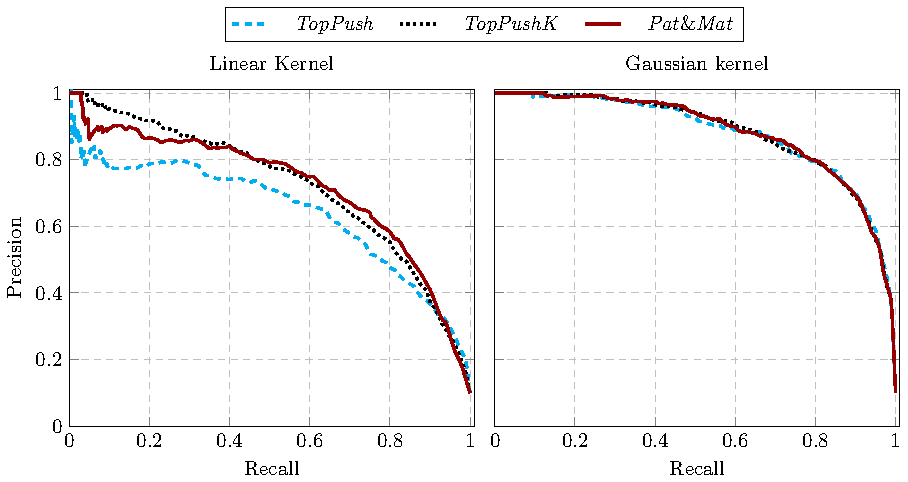
\includegraphics[width = \linewidth]{images/dual_results1.pdf}
  \caption{PR curves for all methods and  FashionMNIST dataset. The left column corresponds to the linear kernel~\eqref{eq:Linear kernel} and the right column corresponds to the Gaussian kernel~\eqref{eq:Gaussian kernel}.}
  \label{fig:PR comparison}
\end{figure}

For a better illustration of how the methods from Figure~\ref{fig:PR comparison} work, we present density estimates of scores $\bm s$ from \eqref{eq:defin_s}. High scores predict positive labels while low scores predict negative labels. The rows of Figure \ref{fig:Scores comparison} depict the linear \eqref{eq:Linear kernel} and the Gaussian kernels \eqref{eq:Gaussian kernel} with~$\sigma = 0.01$ while each column corresponds to one method. The black vertical lines depict the top 5\%-quantile of all scores (on the testing set). Since a smaller overlap of scores of samples with positive and negative labels implies a better separation, we deduce the benefit of the Gaussian over the linear kernel.

\begin{figure}[!ht]
  \centering
  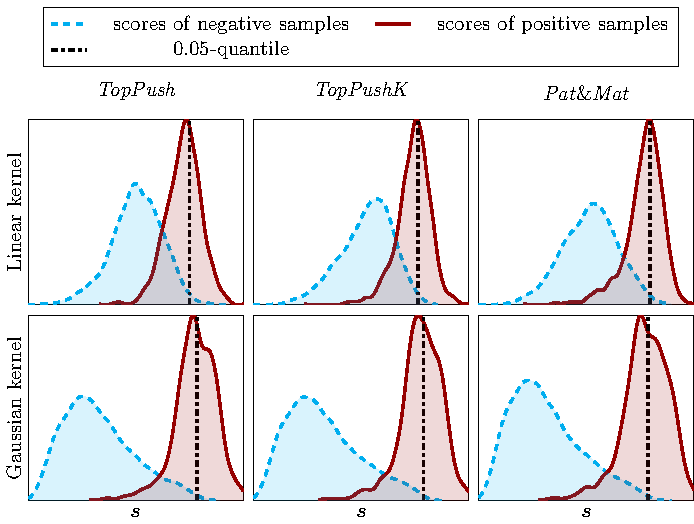
\includegraphics[width = \linewidth]{images/dual_results2.pdf}
  \caption{Density estimates for scores corresponding to samples with positive and negative labels for the FashionMNIST dataset.}
  \label{fig:Scores comparison}
\end{figure}

In Table~\ref{tab:Metrics comparison} we present the precision of all methods across all datasets from Table~\ref{tab:Datasets}. For each dataset, we trained each method and computed precision at certain levels of recall. The depicted values are averages over all datasets. For each kernel and each level of recall, the best precision is highlighted in light green. Moreover, the best overall precision for each level of recall is depicted in dark green. We can make several observations from Table~\ref{tab:Metrics comparison}:
\begin{itemize}
  \item All methods perform better with the Gaussian kernels than with the linear kernel. 
  \item \TopPush and \TopPushK perform better for sufficiently small recall. This happened because they consider the threshold to be the maximal $K$ negative scores and small recall corresponds to high threshold. However, for the same reason, \TopPush is not robust.
  \item \PatMat is the best for all kernels if the recall is sufficiently large. The reason is again the form of the decision threshold.
\end{itemize}

\begin{table}[ht]
  \caption{The precision of all methods averaged across all datasets from Table~\ref{tab:Datasets}. Each column represents precision at a certain level of recall. Light green depicts the best method for the given kernel and dark green depicts the best overall method.}
  \label{tab:Metrics comparison}
  \centering
  \begin{tabular}{@{}c|llllllll@{}}
    \toprule
    \multicolumn{3}{c}{} & \multicolumn{6}{c}{$\pratrec$}  \\
    \cmidrule(lr){4-9}
    \multicolumn{3}{c}{}
      & 0.05 & 0.1 & 0.2 & 0.4 & 0.6 & 0.8 \\
    \midrule
    \multirow{6}{*}{\rotatecell{Linear kernel}}
    & \TopPush
      & & \best 79.83 & 64.27 & \best 65.55 & 61.85 & 57.89 & 51.83 \\
    & \TopPushK & $K = 5$
      & 73.96 & \best 65.41 & 64.82 & 60.28 & 56.94 & 50.52 \\
    & & $K = 10$
      & 60.63 & 61.97 & 59.69 & 56.89 & 54.40 & 49.83 \\
    & \PatMat & $\tau = 0.01$
      & 63.67 & 60.30 & 58.74 & 57.75 & 53.32 & 48.42 \\
    & & $\tau = 0.05$
      & 54.05 & 60.91 & 63.32 & 55.24 & 52.55 & 48.30 \\
    & & $\tau = 0.1$
      & 57.02 & 61.24 & 62.49 & \best 63.11 & \best 59.91 & \best 52.14 \\
    \midrule
    \multirow{6}{*}{\rotatecell{Gaussian kernel}}
    & \TopPush
      & & \besttotal 97.50 & 86.06 & 81.28 & 76.15 & 71.13 & 60.17 \\
    & \TopPushK & $K = 5$
      & 92.50 & 87.56 & 85.31 & 78.47 & 70.77 & 57.10 \\
    & & $K = 10$
      & 89.50 & 87.56 & 83.15 & 79.09 & 71.88 & 59.27 \\
    & \PatMat & $\tau = 0.01$
      & 89.65 & \besttotal 89.11 & \besttotal 86.75 & 80.77 & 75.44 & 65.95 \\
    & & $\tau = 0.05$
      & 80.77 & 81.28 & 85.74 & 82.92 & 74.91 & 65.04 \\
    & & $\tau = 0.1$
      & 81.30 & 84.14 & 82.58 & \besttotal 83.12 & \besttotal 77.82 & \besttotal 66.50 \\
    \bottomrule
  \end{tabular}
\end{table}

In Figure~\ref{fig:Convergence comparison}, we investigate the convergence of methods. In each column, we show the convergence of primal and dual problems for one method. To solve the primal problem, we use the gradient method proposed in~\cite{adam2019patmat}. For the dual problem, we use our Algorithm~\ref{alg:Coordinate descent}. Since~\cite{adam2019patmat} considers only linear kernels, we present them. Moreover, since the computation of the objective is expensive, the results are presented for the sigillito1989classification dataset. We can see that \TopPush and \TopPushK converge to the same objective for primal and dual problems. This means that the problem was solved to optimality. However, there is a little gap between optimal solution of primal and dual problems for \PatMat.

\begin{figure}[!ht]
  \centering
  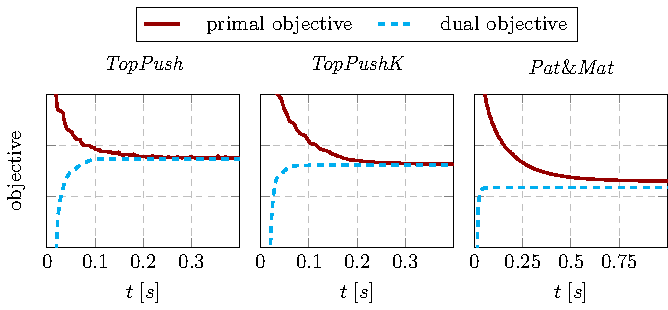
\includegraphics[width = \linewidth]{images/dual_results3.pdf}
  \caption{Convergence of the objectives for the primal (red line) and dual (blue line) problems for the sigillito1989classification dataset with linear kernel.}
  \label{fig:Convergence comparison}
\end{figure}

Finally, Table~\ref{tab:Time comparison} depicts the time comparison for all methods and all datasets. It shows the average time in milliseconds needed for one \repeatloop loop in Algorithm~\ref{alg:Coordinate descent}. The time is relatively stable and for most of the datasets it is below one millisecond. Since we run all experiments for 20000 \repeatloop loops, the evaluation of one method with one hyperparameter setting takes a few seconds for smaller datasets and approximately 7 minutes for FashionMNIST. The average time for one~$\Delta_l$ in step~\ref{alg: line 5} in Algorithm~\ref{alg:Coordinate descent} took between $1.7\cdot 10^{-7}$ and $3.1\cdot 10^{-7}$ seconds for each methods. It is almost the same for all datasets, which corresponds to the fact that the complexity of step~\ref{alg: line 5} is independent of the size of the dataset. Note that in all experiments we used precomputed kernel matrix~$\K$ saved on the hard drive and not in memory.

\begin{table}[ht]
    \caption{The average time with standard deviation (in milliseconds) for one \repeatloop loop in Algorithm~\ref{alg:Coordinate descent}. The average time for one~$\Delta_l$ in step~\ref{alg: line 5} in Algorithm~\ref{alg:Coordinate descent} took between $1.7\cdot 10^{-7}$ and $3.1\cdot 10^{-7}$ seconds for each methods.}
    \label{tab:Time comparison}
    \centering
    \begin{tabular}{@{}c|llll@{}}
        \toprule
        \multicolumn{2}{c}{}
          & \TopPush & \TopPushK & \PatMat \\
        \midrule
        \multirow{5}{*}{\rotatecell{One \repeatloop \\ loop [ms]}}
        & sigillito1989classification
          & $ 0.04 \pm 0.00 $ & $ 0.03 \pm 0.00 $ & $ 0.03 \pm 0.00 $ \\
        & Spambase
          & $ 0.56 \pm 0.02 $ & $ 0.49 \pm 0.01 $ & $ 0.50 \pm 0.01 $ \\
        & WhiteWineQuality
          & $ 0.62 \pm 0.03 $ & $ 0.53 \pm 0.01 $ & $ 0.54 \pm 0.01 $ \\
        & RedWineQuality
          & $ 0.17 \pm 0.01 $ & $ 0.14 \pm 0.01 $ & $ 0.15 \pm 0.01 $ \\
        & Fashion-MNIST
          & $ 17.16 \pm 0.74 $ & $ 15.95 \pm 0.14 $ & $ 15.54 \pm 0.80 $ \\
        \bottomrule
    \end{tabular}
\end{table}

\section{Conclusion}\label{sec:Conclusion}

In this paper, we analyzed and extended the general framework for binary classification on top samples from~\cite{adam2019patmat} to nonlinear problems. Achieved results can be summarized as follows:
\begin{itemize}
    \item We derived the dual formulations for \TopPush, \TopPushK and \PatMat.
    \item We proposed a new method for solving the dual problems. We performed its complexity analysis. For selected surrogate functions we also derived the exact formulas needed in the method.
    \item We performed a numerical analysis of the proposed method. We showed its good convergence as well as improved performance of nonlinear kernels over the linear one.
\end{itemize}
Based on the numerical analysis from Section~\ref{sec:Numerical experiments}, we recommend using \TopPush or \TopPushK for problems where the resulting recall should be small. Otherwise, we recommend using \PatMat with an appropriately selected~$\tau$ parameter.


% ------------------------------------------------------------------------------
% Appendix
% ------------------------------------------------------------------------------
\part*{Apendices}
\appendix

\chapter{Appendix for Chapter~\ref{chap: linear}}
\section{Convexity}

\propconvex*
\begin{proof}[Proof of Proposition~\ref{prop: convexity} on page~\pageref{prop: convexity}]
  From Notation~\ref{not: scores}, threshold~$t_0$ is just a maximum from vector~$\bm{s}^-$ of scores of all negative samples.  Since maximum is a convex function, threshold T is a convex function of weights~$\bm{w}.$ Moreover, it is easy to show that the quantile~$t_1$ is not convex. Due to~\cite{lapin2015top}, the mean of the~$K$ highest values of a vector is a convex function. Therefore, threshold~$t_2$ is a convex function  of weights~$\bm{w}.$ It remains to analyze threshold~$t_3.$ Let us define function~$g$ as follows
  \begin{equation*}
    g(\bm{w},t) := \frac{1}{n} \sum_{i \in \I} l(\bm{w}^{\top} \bm{x}_i - t) - \tau.
  \end{equation*}
  where we for simplicity set~$\vartheta = 1.$ Then~$t_3$ is defined via an implicit equation~$g(\bm{w},t) = 0.$ Moreover, since~$l$ is convex, we immediately obtain that~$g$ is jointly convex in both variables. To show the convexity, consider~$\bm{w}, \; \tilde{\bm{w}} \in \R^d$ and the corresponding thresholds~$t = t_3(\bm{w})$,~$\tilde{t} = t_3(\tilde{\bm{w}})$. Then for any~$\lambda\in[0,1],$ we have 
  \begin{equation}\label{eq:proof_conv1}
    g\Brac{\lambda \bm{w} + (1 - \lambda)\tilde{\bm{w}}, \;\lambda t + (1 - \lambda)\tilde{t}}
    \leq \lambda g(\bm{w}, t) + (1 - \lambda) g(\tilde{\bm{w}}, \tilde{t}) = 0.
  \end{equation}
  The inequality follows from the convexity of~$g$  and the equality from~$g(\bm{w}, t) = g(\tilde{\bm{w}}, \tilde{t}) = 0,$ which holds due to the definition of~$t_3.$ From the definition of~$t_3,$ we also have
  \begin{equation}\label{eq:proof_conv2}
    g(\lambda\bm{w} + (1-\lambda)\tilde{\bm{w}}, \; t_3(\lambda\bm{w} + (1-\lambda)\tilde{\bm{w}})) = 0.
  \end{equation}
  Since~$g$ is non-increasing in the second variable, from~\eqref{eq:proof_conv1} and~\eqref{eq:proof_conv2} we deduce
  \begin{equation*}
    t_3(\lambda\bm{w} + (1-\lambda)\tilde{\bm{w}})
    \leq \lambda t + (1-\lambda)\tilde{t}
    =   \lambda t_3(\bm{w})+(1-\lambda) t_3(\tilde{\bm{w}}),
  \end{equation*}
  which implies that function~$\bm{w}\mapsto t_3(\bm{w})$ is convex.
\end{proof}

\thmconvex*
\begin{proof}[Proof of Theorem~\ref{thm: convexity} on page~\pageref{thm: convexity}]
  Due to the definition~\eqref{eq: confusion counts surrogate}, the objective function~$L$ equals to
  \begin{equation*}
    L(\bm{w}) = \fns(\bm{s}, t(\bm{w})) = \sum_{i \in \Ipos} l \Brac{t(\bm{w}) - \bm{w}^{\top} \bm{x}_i}.
  \end{equation*}
  Here we write~$t(\bm{w})$ to stress the dependence of~$t$ on~$\bm{w}$. Since~$\bm{w}\mapsto t(\bm{w})$ is a convex function, we also have that~$\bm{w} \mapsto t(\bm{w}) - \bm{w}^{\top} \bm{x}$ is a convex function. From its definition, the surrogate function~$l$ is convex and non-decreasing.  Since the composition of a convex function with a non-decreasing convex function is a convex function, this finishes the proof.
\end{proof}

\section{Differentiability}

\derivative* 
\begin{proof}[Proof of Theorem~\ref{thm: differentiability} on page~\pageref{thm: differentiability}]
  The non-differentiability of~$t_0,$~$t_1$ and~$t_2$ happens whenever the threshold value is achieved at two different scores. The result for~$t_3$ follows directly from the implicit function theorem. 
\end{proof}

\newpage

\section{Stability}\label{app: stability}

\degeneratebehavior*

Additionally to the assumptions from Example~\ref{ex: degenerate behaviour}, we consider the hinge loss function and no regularization for all formulations from Table~\ref{tab: summary formulations}. We also assume that~$n$ is large, and the outlier may be ignored for the computation of thresholds that require a large number of points. Since the computation is simple for other formulations, we show it only for \PatMat. For~$\bm{w}_0 = (0,0),$ we have
\begin{equation*}
  \tau
  = \frac{1}{n}\sum_{i \in \I} l\Brac{\vartheta(\bm{w}_0^\top \bm{x}_i - t)}
  = l(0 - \vartheta t) = 1 - \vartheta t,
\end{equation*}
which implies that threshold~$t$ equals~$t = \nicefrac{1-\tau}{\vartheta}.$ Consequently, the value of the objective function is
\begin{equation}\label{eq: PatMat objective 0}
  L(\bm{w}_0)
    = \frac{1}{\npos} \sum_{i \in \Ipos} l(t - \bm{w}_0^\top \bm{x}_i)
    = l(t - 0)
    = 1 + t,
\end{equation}
where the last equality follows from the definition of the hinge loss function and the fact that~$t \geq 0.$ This finishes the computation for~$\bm{w}_0$. For~$\bm{w}_1 = (1,0),$ the computation goes similar. Since all samples are uniformly distributed in~$[-1,1]\times[-1,1],$ scores~$\bm{w}_1^\top \bm{x}_i$ for~$i \in \I$ are uniformly distributed in~$[-1,1].$ Then, if the scaling parameter~$\vartheta$ satisfies~$\vartheta \leq \tau$, we have
\begin{align*}
  \tau
    & = \frac{1}{n} \sum_{i \in \I} l\Brac{\vartheta (\bm{w}_1^\top \bm{x}_i - t)}
    \approx \frac{1}{2}\int_{-1}^{1} l\Brac{\vartheta(s-t)} \dd{s}
      = \frac{1}{2} \int_{-1}^{1} \max\{0, 1 + \vartheta(s - t)\}\dd{s} \\
    & =\frac{1}{2} \int_{-1}^{1} (1+\vartheta(s - t))\dd{s}
      = 1 - \vartheta t + \frac{\vartheta}{2}\int_{-1}^{1}s\dd{s}
      = 1 - \vartheta t.
\end{align*}
which again implies that threshold~$t$ equals~$t = \nicefrac{1-\tau}{\vartheta}$. Note that we could ignore the~$\max$ operator in the relation above, since 
\begin{equation*}
  1 + \vartheta(s - t)
    \geq 1 + \vartheta(-1 - t)
    = 1 + \vartheta(-1 - \frac{1 - \tau}{\vartheta})
    = \tau - \vartheta
    \geq 0.
\end{equation*}
Finally, since positive samples are uniformly distributed in~$[0,1]\times[-1,1],$ corresponding scores $\bm{w}_1^\top \bm{x}_i$  for~$i \in \Ipos$ are uniformly distributed in~$[0,1].$ Therefore, for the objective function, we have
\begin{equation*}
  L(\bm{w}_1)
    = \frac{1}{\npos} \sum_{i \in \Ipos} l(t - \bm{w}_1^\top \bm{x}_i)
    \approx \int_{0}^{1} l(t-s)\dd{s}
    = \int_{0}^{1} (1 + t - s)\dd{s}
    = 0.5 + t.
\end{equation*}
Results for \PatMatNP can be obtained in a similar way.

\pagebreak

\larget*
\begin{proof}[Proof of Theorem~\ref{thm:large_t} on page~\pageref{thm:large_t}]
  All mentioned formulations use surogate approximation of the false-negative rate as the objective function~$L.$ For the linear classifier, the objective function has the following form
  \begin{equation*}
    L(\bm{w})
      = \frac{1}{\npos}\sum_{i \in \Ipos}l(t - \bm{w}^{\top} \bm{x}_i)
  \end{equation*}
  Due to~$l(0) = 1$ and the convexity of~$l$ we have~$l(s) \geq 1 + cs$, where~$c$ equals to the derivative of~$l$ at~$0$. Then we have
  \begin{equation*}
    L(\bm{w}) 
      \geq \frac{1}{\npos} \sum_{i \in \Ipos}(1 + c(t-\bm{w}^{\top} \bm{x}_i))
      = 1 + c\Brac{t - \frac{1}{\npos}\sum_{i \in \Ipos}\bm{w}^{\top} \bm{x}}
      \geq 1,
  \end{equation*}
  where the last inequality follows from assumption~\eqref{eq:w_zero_nn}. Now we realize that for any formulation from the statement, the corresponding threshold for~$\bm{w}=0$ equals to~$t=0$, and thus~$L(\bm{0})=1$. But then~$L(\bm{0}) \leq L(\bm{w})$. The second part of the result follows from the form of thresholds~$t(\bm{w})$.
\end{proof}

\patmatzero*
\begin{proof}[Proof of Theorem~\ref{thm:patmat_zero} on page~\pageref{thm:patmat_zero}]
  Firstly recall thewe use linear model and Notation~\ref{not: scores} and define the following auxilliary variables
  \begin{equation*}
    \begin{aligned}
      s_{\min} & = \min \Set{s_i}{i \in \I}, \qquad
      s_{\max} & = \max \Set{s_i}{i \in \I}, \qquad
      \bar{s} & = \frac{1}{n} \sum_{i \in \I} s_i. \\
    \end{aligned}
  \end{equation*}
  Using the definition of~$\bar{s}$ we get the following relation
  \begin{equation}\label{eq:patmat_zero_aux0}
    \bar{s}
      = \frac{1}{n} \sum_{i \in \I} s_i
      = \frac{1}{n}\sum_{i \in \Ipos} s_i + \frac{1}{n} \sum_{i \in \Ineg} s_i
      < \frac{1}{n} \sum_{i \in \Ipos} s_i + \frac{\nneg}{n\npos} \sum_{i \in \Ipos} s_i
      = \frac{1}{\npos} \sum_{i \in \Ipos} s_i,
  \end{equation}
  where the inequality follows from~\eqref{eq:patmat_zero} and the last equality follows from
  \begin{equation*}
    \frac{1}{n} + \frac{\nneg}{n\npos}
      = \frac{1}{n} \Brac{1 + \frac{\nneg}{\npos}} 
      = \frac{1}{n} \frac{\npos + \nneg}{\npos}
      = \frac{1}{n} \frac{n}{\npos}
      = \frac{1}{\npos}.
  \end{equation*}
  Moreover, since the average of elements of the  vector is smaller or equal to the maximum of elements of the same vector, we get the following relation
  \begin{equation*}
    \bar{s}
      < \frac{1}{\npos} \sum_{i \in \Ipos} s_i
      \leq \max \Set{s_i}{i \in \Ipos}
      \leq \max \Set{s_i}{i \in \I}
      = s_{\max}
  \end{equation*}
  where the first inequality follows from~\eqref{eq:patmat_zero_aux0}. The lower bound for~$\bar{s}$ can be computed in a similar way. Altogether, we have~$s_{\min} < \bar{s} < s_{\max}$. Then we can define
  \begin{equation*}
    \vartheta_0 = \min\Brac[c]{\frac{\tau}{\bar{s} - s_{\min}}, \; \frac{1-\tau}{s_{\max}-\bar{s}}, \; \tau},
  \end{equation*}
  observe that~$\vartheta_0 > 0$, fix any~$\vartheta \in (0, \vartheta_0)$ and define
  \begin{equation*}
    t = \frac{1 - \tau}{\vartheta} + \bar{s}.
  \end{equation*}
  Then we obtain for any~$i \in \I$
  \begin{equation*}
    1 + \vartheta(s_i - t)
      \geq 1 + \vartheta(s_{\min} - t)
      = 1 + \vartheta s_{\min} - 1 + \tau - \vartheta\bar{s}
      = \tau - \vartheta (\bar{s} - s_{\min}),
  \end{equation*}
  where the first equality follows from the definition of~$t.$ From the definition~$\vartheta_0$ we known the following
  \begin{equation*}
    0 < \vartheta \leq \vartheta_0 \leq \frac{\tau}{\bar{s} - s_{\min}}.
  \end{equation*}
  Since~$\bar{s} - s_{\min} > 0,$ we get the following inequality
  \begin{equation}\label{eq:patmat_zero_aux1}
    1 + \vartheta(s_i - t)
      = \tau - \vartheta (\bar{s} - s_{\min})
      \geq \tau - \frac{\tau}{\bar{s} - s_{\min}} (\bar{s} - s_{\min})
      = 0
  \end{equation}
  Moreover, combining the definition of the hinge loss function in Notation~\ref{not: surrogates} and the inequality above, we have
  \begin{equation*}
    l\Brac{\vartheta (s_i - t)} = \max\{0, 1 + \vartheta (s_i - t), 0\} = \Brac{1 + \vartheta(s_i - t)}.
  \end{equation*}
  Finally, replacing the hinge loss in the left hand side of~\eqref{eq: aatp quantile surrogate} leads to
  \begin{equation*}
    \begin{aligned}
      \frac{1}{n} \sum_{i \in \I} l\Brac{\vartheta (s_i - t)}
      & = \frac{1}{n}\sum_{i \in \I}\Brac{1 + \vartheta(s_i - t)} \\
      & = 1 - \vartheta t + \frac{\vartheta}{n} \sum_{i \in \I} s_i \\
      & = 1 - \vartheta \Brac{\frac{1 - \tau}{\vartheta} + \bar{s}} + \vartheta \bar{s} \\
      & = \tau,
    \end{aligned}
  \end{equation*}
  where the third equality employs the definition of~$\bar{s}$ and~$t$. But this means that~$t$ is the threshold corresponding to~$\bm{w}$, i.e. it solves~\eqref{eq: aatp quantile surrogate}. Similarly to~\eqref{eq:patmat_zero_aux1} we get
  \begin{equation}\label{eq:patmat_zero_aux2}
    1 + t - s_i
    \geq 1 + t-s_{\max}
    =   1 + \frac{1-\tau}{\vartheta} + \bar{s} - s_{\max}
    \geq \frac{1-\tau}{\vartheta} + \bar{s} - s_{\max}
    \geq 0,
  \end{equation}
  where the last inequality follows from the definition of~$\vartheta_0$. Then for the objective we have
  \begin{equation*}
    \begin{aligned}
      L(\bm{w}) = \frac{1}{\npos}\sum_{i \in \Ipos}l(t-s_i)
      & = \frac{1}{\npos}\sum_{i \in \Ipos}\Brac{1+t-s_i} \\
      & = 1 + t - \frac{1}{\npos}\sum_{i \in \Ipos} s_i \\
      & < 1 + \Brac{\frac{1 - \tau}{\vartheta} + \bar{s}} - \bar{s} \\
      & = 1 + \frac{1-\tau}{\vartheta} \\
      & = L(\bm{0}),\\
    \end{aligned}
  \end{equation*}
  where the second equality follows from~\eqref{eq:patmat_zero_aux2}, the only inequality from~\eqref{eq:patmat_zero_aux0} and the last equality from~\eqref{eq: PatMat threshold 0} and~\eqref{eq: PatMat objective 0}. Thus, we finished the proof for \PatMat. The proof for \PatMatNP can be performed in an identical way by replacing in the definition of~$\bar{s}$ the mean with respect to all samples by the mean with respect to all negative samples.
\end{proof}

\section{Threshold comparison}\label{app:relations}

Whenever the objective contains only false-negatives, a lower threshold~$t$ means a lower objective function. Therefore, a lower threshold is preferred. The two following lemmas compares thresholds defined in Chapter~\ref{chap: framework} in terms of approximation quality.
\begin{lemma}[Thresholds relation~\cite{zhang2018tau}]\label{prop: threholds}
  We always have
  \begin{equation*}
    t_1(\bm{s}) \leq t_2(\bm{s}) \leq t_3(\bm{s}).
  \end{equation*}
\end{lemma}



\begin{lemma}\label{lemma:thresholds2}
  Consider the \Grill, \GrillNP, \TopMeanK and \tauFPL formulations and the notation from Notation~\ref{not: scores}. Then we have the following statements:
  \begin{equation*}
    \begin{aligned}
      s_{[\npos\tau]}^+ > s_{[\nneg\tau]}^-
        & \implies \Grill \text{ has larger threshold than }\GrillNP, \\
      \frac{1}{\npos\tau}\sum_{i=1}^{\npos\tau} s_{[i]}^+
      > \frac{1}{\nneg\tau}\sum_{i=1}^{\nneg\tau} s_{[i]}^-
        & \implies \TopMeanK \text{ has larger threshold than }\tauFPL. \\
    \end{aligned}
  \end{equation*}
\end{lemma}

\begin{proof}
  Since~$\bm{s}^+$ and~$\bm{s}^-$ are computed on disjunctive indices, we have
  \begin{equation*}
    s_{[n\tau]} \geq \min\{s_{[\npos\tau]}^+, \; s_{[\nneg\tau]}^-\}.
  \end{equation*}
  Since~$s_{[n\tau]}$ is the threshold for \Grill and~$s_{[\nneg\tau]}^-$ is the threshold for \GrillNP, the first statement follows. The second part can be shown in a similar way.
\end{proof}
  
\noindent Since the goal of the presented formulations is to push~$s^+$ above~$s^-$, we may expect that the conditions in Lemma~\ref{lemma:thresholds2} hold true. 

\section{Computing the threshold for \PatMat}\label{app:threshold}

We show how to efficiently compute the threshold~\eqref{eq: aatp quantile surrogate} for \PatMat with linear model and the hinge surrogate from Notation~\ref{not: surrogates}. Consider function
\begin{equation}\label{eq:defin_h}
  h(t) = \sum_{i \in \I} l\Brac{\vartheta(s_i - t)} - n\tau.
\end{equation}
Then solving~\eqref{eq:update_t} is equivalent to looking for~$\hat{t}$ such that~$h(\hat{t}) = 0$. Function~$h$ is continuous and strictly decreasing (until it hits the global minimum) with~$h(t) \to \infty$ as~$t \to -\infty$ and~$h(t) \to -n\tau$ as~$t \to \infty$. Thus, there is a unique solution to the equation~$h(t) = 0$. For sorted data, the following lemma gives advice on how to solve equation~$h(t) = 0$. 

\begin{lemma}
  Consider vector of scores~$\bm{s}$ and its sorted version~$\bm{s}_{[\cdot]}$ with decreasing elements as defined in Notation~\ref{not: scores}. Define~$\gamma = \nicefrac{1}{\vartheta}$. Then 
  \begin{equation}\label{eq:update_h}
    h(s_{[j]} + \gamma) = h(s_{[j - 1]} + \gamma) + (j - 1) \vartheta(s_{[j - 1]} - s_{[j]})
  \end{equation}
  for all~$i = 2, \; 3, \ldots, n$ with the initial condition~$h(s_{[1]} + \gamma) = -n\tau$.
\end{lemma}
\begin{proof}
Observe first that
\begin{equation*}
  \begin{aligned}
    h(s_{[j]}+\gamma)
      & = \sum_{i \in \I} l\Brac{\vartheta(s_i - (s_{[j]} + \gamma))} - n\tau \\
      & = \sum_{i \in \I} \max\Brac[c]{0,\; 1 + \vartheta\Brac{s_i - s_{[j]} - \frac{1}{\gamma}}} - n\tau \\
      & = \sum_{i = 1}^{j - 1} \vartheta(s_{[i]} - s_{[j]}) - n\tau,
  \end{aligned}
\end{equation*}
where the last equality holds since~$\vartheta > 0$ and~$s_{[i]} - s_{[j]} \leq 0$ for all~$i \geq j$
From here, we obtain~$h(s_{[1]} + \gamma) = -n\tau$. Moreover, we have
\begin{equation*}
  \begin{aligned}
    h(s_{[j]} + \gamma)
    & = \sum_{i = 1}^{j - 1} \vartheta(s_{[i]} - s_{[j]}) - n\tau \\
    & = \sum_{i = 1}^{j - 2} \vartheta(s_{[i]} - s_{[j]}) + \vartheta(s_{[j-1]} - s_{[j]}) - n\tau \\
    & = \sum_{i = 1}^{j - 2} \vartheta(s_{[i]} - s_{[j]} \pm s_{[j - 1]}) + \vartheta(s_{[j-1]} - s_{[j]}) - n\tau \\
    & = \sum_{i = 1}^{j - 2} \vartheta(s_{[i]} - s_{[j - 1]}) + \sum_{i = 1}^{j - 2} \vartheta(s_{[j - 1]} - s_{[j]}) + \vartheta(s_{[j - 1]} - s_{[j]}) - n\tau \\
    & = h(s_{[j - 1]} + \gamma) + (j - 1) \vartheta(s_{[j - 1]} - s_{[j]}),
  \end{aligned}
\end{equation*}
which finishes the proof.
\end{proof}

\noindent Thus, to solve~$h(t) = 0$ with the hinge surrogate, we start with~$t_1 = s_{[1]}  + \gamma$ and~$h(t_1) = -n\tau$. Then we start decreasing~$t$ according to~\eqref{eq:update_h} until we find some~$t_i = s_{[i]} + \gamma$ such that~$h(t_i) > 0$. The desired~$t$ then lies between~$t_i$ and~$t_{i-1}$. Since~$h$ is a piecewise linear function with
\begin{equation*}
  h(t) = h(t_{i-1}) + \frac{t - t_{i-1}}{t_{i} - t_{i-1}}\Brac{h(t_{i}) - h(t_{i-1})}
\end{equation*}
for~$t \in [t_{i-1}, \; t_{i}]$, the precise value of~$\hat{t}$ can be computed by a simple interpolation
\begin{equation*}
  \hat{t}
    = t_{i-1} - h(t_{i-1})\frac{t_{i} - t_{i-1}}{h(t_{i}) - h(t_{i-1})}
    = t_{i-1} - h(t_{i-1})\frac{t_{i} - t_{i-1}}{-(i-1)\vartheta(t_{i} - t_{i-1})}
    = t_{i-1} + \frac{h(t_{i-1})}{\vartheta(i-1)}.
\end{equation*}

\section{Convergence of stochastic gradient descent}

The proof is divided into three parts. In Section~\ref{app:sgd1}, we prove a general statement for convergence of stochastic gradient descent with a convex objective. In Section~\ref{app:sgd2} we apply it to Theorem~\ref{thm:sgd}. The proof is based on auxiliary results from Section~\ref{app:sgd3}.

\subsection{General result}\label{app:sgd1}

Consider a differentiable objective function~$L$ and the optimization method
\begin{equation}\label{eq:update}
  \bm{w}^{k+1} = \bm{w}^k - \alpha^k g(\bm{w}^k),
\end{equation}
where~$\alpha^k > 0$ is a stepsize and~$g(\bm{w}^k)$ is an approximation of the gradient~$\nabla L(\bm{w}^k)$. Assume the following:
\begin{enumerate}[label={(A\arabic*)}]
  \item \label{ass_convex}~$L$ is differentiable, convex and attains a global minimum;
  \item \label{ass_gbound}~$\norm{g(\bm{w}^k)}\leq B$ for all~$k$;
  \item \label{ass_alpha1} the stepsize is non-increasing and satisfies~$\sum_{k=0}^\infty \alpha^k = \infty$;
  \item \label{ass_alpha2} the stepsize satisfies~$\sum_{k=0}^\infty (\alpha^k)^2<\infty$;
  \item \label{ass_alpha3} the stepsize satisfies~$\sum_{k=0}^\infty \norm{\alpha^{k+1}-  \alpha^k}<\infty$.
\end{enumerate}
Assumptions~\ref{ass_alpha1}-\ref{ass_alpha3} are satisfied for example for~$\alpha^k = \nicefrac{\alpha^0}{k+1}$. We start with the general result.

\begin{theorem}\label{thm:convergence}
  Assume that~\ref{ass_convex}-\ref{ass_alpha2} is satisfied. If there exists some~$C$ such that for some global minimum of~$\bm{w}^*$ of~$L$ we have
  \begin{equation}\label{eq:nec_cond}
    \sum_{k=0}^\infty \alpha^k \inner{g(\bm{w}^k) - \nabla L(\bm{w}^k)}{\bm{w}^* - \bm{w}^k} \leq C,
  \end{equation}
  then the sequence~$\{\bm{w}^k\}$ generated by~\eqref{eq:update} is bounded and~$L(\bm{w}^k) \to L(\bm{w}^*)$. Thus, all its convergent subsequences converge to some global minimum of~$L$.
\end{theorem}
\begin{proof}
  Note first that the convexity of~$L$ from~\ref{ass_convex} implies
  \begin{equation}\label{eq:convex_estimate}
    \inner{\nabla L(\bm{w}^k)}{\bm{w}^* - \bm{w}^k} \leq L(\bm{w}^*) - L(\bm{w}^k).
  \end{equation}
  Then we have
  \begin{equation*}
    \begin{aligned}
      \norm{\bm{w}^{k+1} - \bm{w}^*}^2
        = \; & \norm{\bm{w}^k - \alpha^k g(\bm{w}^k) - \bm{w}^*}^2 \\
        = \; &\norm{\bm{w}^k - \bm{w}^*}^2 + 2\alpha^k\inner{g(\bm{w}^k)}{\bm{w}^* - \bm{w}^k} + (\alpha^k)^2 \norm{g(\bm{w}^k)}^2 \\
        \leq \; &\norm{\bm{w}^k - \bm{w}^*}^2 + 2\alpha^k\inner{g(\bm{w}^k) \pm \nabla L(\bm{w}^k)}{\bm{w}^* - \bm{w}^k} + (\alpha^k)^2 B^2\\
        \leq \; & \norm{\bm{w}^k - \bm{w}^*}^2 + 2 \alpha^k \inner{g(\bm{w}^k) - \nabla L(\bm{w}^k)}{\bm{w}^* - \bm{w}^k} \\
        & + 2 \alpha^k \Brac{L(\bm{w}^*) - L(\bm{w}^k)} + (\alpha^k)^2 B^2,
    \end{aligned}
  \end{equation*}
  where the first inequality follows from assumption~\ref{ass_gbound} and the second on from the properties of inner product and~\eqref{eq:convex_estimate}. Summing this expression for all~$k$ and using~\eqref{eq:nec_cond} leads to
  \begin{equation*}
    \limsup_{k \rightarrow \infty} \; \norm{\bm{w}^k - \bm{w}^*}^2
      \leq \norm{\bm{w}^0 - \bm{w}^*}^2 + 2C + 2 \sum_{k=0}^\infty \alpha^k (L(\bm{w}^*) - L(\bm{w}^k)) + \sum_{k=0}^ \infty (\alpha^k)^2 B^2.
\end{equation*}
  Using assumption~\ref{ass_alpha2} results in the existence of some~$\hat{C}$ such that
  \begin{equation}\label{eq:general_bound}
  \limsup_{k \rightarrow \infty} \;\norm{\bm{w}^k - \bm{w}^*}^2 + 2\sum_{k=0}^\infty \alpha^k \Brac{L(\bm{w}^k) - L(\bm{w}^*)} \leq 2 \hat{C}.
  \end{equation}
  Since~$\alpha^k > 0$ and~$L(\bm{w}^k) \geq L(\bm{w}^*)$ as~$\bm{w}^*$ is a global minimum of~$L$, we infer that sequence~$\{\bm{w}^k\}$ is bounded and~\eqref{eq:general_bound} implies
  \begin{equation*}
    \sum_{k=0}^\infty \alpha^k \Brac{L(\bm{w}^k) - L(\bm{w}^*)} \leq \hat{C}.
  \end{equation*}
  Since~$L(\bm{w}^k) - L(\bm{w}^*) \geq 0$, due to assumption~\ref{ass_alpha1} we obtain
  \begin{equation*}
    \lim_{k \to \infty} L(\bm{w}^k) = L(\bm{w}^*),
  \end{equation*}
  which implies the theorem statement.
\end{proof}

\subsection{Proof of Theorem~\ref{thm:sgd}}\label{app:sgd2}

For the proof, we will consider a general surrogate which satisfies:
\begin{enumerate}[label={(S\arabic*)}]
  \item \label{surr_basic1} $l(s)\geq 0$ for all~$s\in\R$, $l(0)=1$ and~$l(s)\to 0$ as~$s\to-\infty$;
  \item \label{surr_basic2} $l$ is convex and strictly increasing function on~$(s_0,\infty)$, where~$s_0:=\sup\{s \mid l(s)=0\}$;
  \item \label{surr_ratio} $\nicefrac{l'}{l}$ is a decreasing function on~$(s_0,\infty)$;
  \item \label{surr_der1} $l'$ is a bounded function;
  \item \label{surr_der2} $l'$ is a Lipschitz continuous function with Lipschitz constant~$D$.
\end{enumerate}
All these reguirements are satisfied for the surrogate logistic or by the Huber loss, which is the hinge surrogate which is smoothened on an~$\varepsilon$-neighborhood of zero.

\sgd*
\begin{proof}[Proof of Theorem~\ref{thm:sgd} on page~\pageref{thm:sgd}]
  We intend to apply Theorem~\ref{thm:convergence} and thus, we need to verify its assumptions. Assumption~\ref{ass_convex} is satisfied as~$L$ is convex due to Theorem~\ref{thm: convexity}. Assumption~\ref{ass_gbound} follows directly from Lemma~\ref{lemma:bound_g}. Assumptions~\ref{ass_alpha1},\ref{ass_alpha2} and~\ref{ass_alpha3} are imposed directly in the statement of this theorem. It remains to verify~\eqref{eq:nec_cond}.

  For simplicity, we will do so only for~$\vartheta = 1$ and for~$2$ minibatches of the same size. However, the proof would be identical for other values. This implies that there are some~$\Imb^k$ and~$\Imb^{k+1}$ which are pairwise disjoint, they cover all samples and that~$\Imb^k = \Imb^{k+2}$ for all~$k$. The assumptions imply that the number of positive samples in each minibatch equal to~$\nmbpos^k = \nicefrac{\npos}{2}$, where~$\npos$ is the total number of positive samples.

  First we estimate the difference between~$s_i^k$ defined in~\eqref{eq:defin_z} and~$\bm{x}_i^\top \bm{w}^k$. For any~$i \in \Imb^k$ we have
  \begin{equation*}
    s_i^k = \bm{x}_i^\top \bm{w}^k
  \end{equation*}
  and since we have two disjoint minibatches, due to the construction~\eqref{eq:defin_z} we get
  \begin{equation}\label{eq:sgd_estimate_z1}
    \begin{aligned}
      s_i^{k-1}
          = s_i^{k-2}
        & = \bm{x}_i^\top \bm{w}^{k-2} \\
        & = \bm{x}_i^\top \Brac{\bm{w}^k + \alpha^{k-2}g(\bm{w}^{k-2}) + \alpha^{k-1} g(\bm{w}^{k-1})} \\
        & = \bm{x}_i^\top \bm{w}^k + \alpha^{k-2}\bm{x}_i^\top g(\bm{w}^{k-2}) + \alpha^{k-1}\bm{x}_i^\top g(\bm{w}^{k-1}).
    \end{aligned}
  \end{equation}
  Similarly, due to the construction~\eqref{eq:defin_z}, for~$i \notin \Imb^k$ we have
  \begin{equation}\label{eq:sgd_estimate_z2}
    s_i^k
    = s_i^{k-1}
    = \bm{x}_i^\top \bm{w}^{k-1}
    = \bm{x}_i^\top (\bm{w}^k+\alpha^{k-1}g(\bm{w}^{k-1}))
    = \bm{x}_i^\top \bm{w}^k + \alpha^{k-1}\bm{x}_i^\top g(\bm{w}^{k-1}).
  \end{equation}
  Recall that we already verified~\ref{ass_convex}-\ref{ass_alpha3}. Combining~\ref{ass_gbound} with~\eqref{eq:sgd_estimate_z1} and~\eqref{eq:sgd_estimate_z2} yields the existence of some~$C_2$ such that for all~$i \in \I$ we have
  \begin{equation}\label{eq:estimate_diff_z}
    \begin{aligned}
      \norm{s_i^k - \bm{x}_i^\top \bm{w}^k} &\leq C_2\alpha^{k-1}, \\
      \norm{s_i^{k-1} - \bm{x}_i^\top \bm{w}^k} &\leq C_2\Brac{\alpha^{k-1}+\alpha^{k-2}}. \\
    \end{aligned}
  \end{equation}
  This also immediately implies
  \begin{equation}\label{eq:estimate_diff_t}
    \begin{aligned}
      \norm{t^k - t(\bm{w}^k)}     & \leq C_2\alpha^{k-1}, \\
      \norm{t^{k-1} - t(\bm{w}^k)} & \leq C_2\Brac{\alpha^{k-1}+\alpha^{k-2}}. \\
    \end{aligned}
  \end{equation}
  Since~$l'$ is Lipschitz continuous with Lipschitz constant~$D$ according to~\ref{surr_der2}, due to~\eqref{eq:estimate_diff_z} and~\eqref{eq:estimate_diff_t} we get
  \begin{equation}\label{eq:sgd_lipschitz1}
    \begin{aligned}
      \norm{l'(t^k-s_i^k) - l'(t(\bm{w}^k)-\bm{x}_i^\top \bm{w}^k)}
        & \leq D \norm{t^k-s_i^k - t(\bm{w}^k)+ \bm{x}_i^\top \bm{w}^k}
        \leq  2C_2 D \alpha^{k-1}.
    \end{aligned}
  \end{equation}
  In an identical way we can show
  \begin{equation}\label{eq:sgd_lipschitz2}
    \begin{aligned}
      \norm{l'(t^{k-1}-s_i^{k-1}) - l'(t(\bm{w}^k)-\bm{x}_i^\top \bm{w}^k)}
        & \leq 2C_2D\Brac{\alpha^{k-1}+\alpha^{k-2}}, \\
      \norm{l'(s_i^k-t^k) - l'(\bm{x}_i^\top \bm{w}^k-t(\bm{w}^k))}
        & \leq 2C_2D\alpha^{k-1}, \\
      \norm{l'(s_i^{k-1}-t^{k-1}) - l'(\bm{x}_i^\top \bm{w}^k-t(\bm{w}^k))}
        & \leq 2C_2D\Brac{\alpha^{k-1}+\alpha^{k-2}}.
    \end{aligned}
  \end{equation}
  Now we need to estimate the distance between~$\nabla t(\bm{w}^k)$ and~$\nabla t^k$. From~\eqref{eq:update_nablat} and~\eqref{eq:update_a}, we have
  \begin{equation*}
    \nabla t^k
      = \frac{\sum_{i \in \Imb^k} l'(s_i^k - t^k)\bm{x}_i + \sum_{i \in \Imb^{k-1}} l'(s_i^{k-1} - t^{k-1}) \bm{x}_i}{\sum_{i \in \I} l'(s_i^k - t^k)}.
  \end{equation*}
  Moreover, using Theorem~\ref{thm: differentiability} and the fact that we have only two minibatches and therefore for any~$k$ we have~$\I = \Imb^k \cup \Imb^{k-1}$, we get
  \begin{equation*}
    \nabla t(\bm{w}^k)
      = \frac{\sum_{i \in \Imb^k} l'(\bm{x}_i^\top \bm{w}^k - t(\bm{w}^k))\bm{x}_i + \sum_{i \in \Imb^{k-1}} l'(\bm{x}_i^\top \bm{w}^k - t(\bm{w}^k))\bm{x}_i}{\sum_{i \in \I} l'(\bm{x}_i^\top \bm{w}^k - t(\bm{w}^k))}.
  \end{equation*}
  From Lemma~\ref{lemma:bound_zero} we deduce that the denominators in the relations above are bounded away from zero uniformly in~$k$. Assumption~\ref{ass_alpha2} implies ~$\alpha^k \to 0$. This allows us to use Lemma~\ref{lemma:ratio} which together with~\eqref{eq:sgd_lipschitz2} implies that there is some~$C_3$ such that for all sufficiently large~$k$ we have
  \begin{equation}\label{eq:sgd_nablat_diff}
    \norm{\nabla t^k - \nabla t(\bm{w}^k)} \leq C_3\Brac{\alpha^{k-1} + \alpha^{k-2}}.
  \end{equation}
  Using the assumptions above, we can simplify the terms for~$g(\bm{w}^k)$ and~$\nabla L(\bm{w}^k)$ to
  \begin{equation*}
    \begin{aligned}
      g(\bm{w}^k)
        & = \frac{2}{\npos} \sum_{i \in \Imbpos^k} l'(t^k - s_i^k)(\nabla t^k - \bm{x}_i), \\
      g(\bm{w}^{k+1})
        & = \frac{2}{\npos} \sum_{i \in \Imbpos^{k+1}} l'(t^{k+1}-s_i^{k+1})(\nabla t^{k+1} - \bm{x}_i), \\
      \nabla L(\bm{w}^k)
        & = \frac{1}{\npos} \sum_{i \in \Ipos} l'(t(\bm{w}^k) - \bm{x}_i^\top \bm{w}^k)(\nabla t(\bm{w}^k) - \bm{x}_i), \\
      \nabla L(\bm{w}^{k+1})
        & = \frac{1}{\npos} \sum_{i \in \Ipos} l'(t(\bm{w}^{k+1}) - \bm{x}_i^\top \bm{w}^{k+1})(\nabla t(\bm{w}^{k+1}) - \bm{x}_i).
    \end{aligned}
  \end{equation*}
  Due to the assumptions, we have~$\Ipos = \Imbpos^k \cup \Imbpos^{k+1}$ and~$\emptyset = \Imbpos^k \cap \Imbpos^{k+1}$, which allows us to write
  \begin{subequations}\label{eq:sgd_sum}
    \begin{align}
    \label{eq:sgd_sum1}
    \npos & \Brac{g(\bm{w}^k) + g(\bm{w}^{k+1}) - \nabla f(\bm{w}^k)-\nabla f(\bm{w}^{k+1})}\\
    \label{eq:sgd_sum2}
    & = \sum_{i \in \Imbpos^k} l'(t^k - s_i^k)(\nabla t^k - \bm{x}_i) - \sum_{i \in \Imbpos^k} l'(t(\bm{w}^k) - \bm{x}_i^\top \bm{w}^k)(\nabla t(\bm{w}^k) - \bm{x}_i) \\
    \label{eq:sgd_sum3}
    & + \sum_{i \in \Imbpos^k} l'(t^k - s_i^k)(\nabla t^k - \bm{x}_i) - \sum_{i \in \Imbpos^k} l'(t(\bm{w}^{k+1}) - \bm{x}_i^\top \bm{w}^{k+1})(\nabla t(\bm{w}^{k+1}) - \bm{x}_i)\\
    \label{eq:sgd_sum4}
    & + \sum_{i \in \Imbpos^{k+1}} l'(t^{k+1} - s_i^{k+1})(\nabla t^{k+1} - \bm{x}_i) - \sum_{i\in \Imbpos^{k+1}}l'(t(\bm{w}^k) - \bm{x}_i^\top \bm{w}^k)(\nabla t(\bm{w}^k) - \bm{x}_i) \\
    \label{eq:sgd_sum5}
    & + \sum_{i \in \Imbpos^{k+1}} l'(t^{k+1} - s_i^{k+1})(\nabla t^{k+1} - \bm{x}_i)  - \sum_{i \in \Imbpos^{k+1}} l'(t(\bm{w}^{k+1}) - \bm{x}_i^\top \bm{w}^{k+1})(\nabla t(\bm{w}^{k+1}) - \bm{x}_i).
    \end{align}
  \end{subequations}
  Then relations~\eqref{eq:sgd_nablat_diff} and~\eqref{eq:sgd_lipschitz1} applied to Lemma~\ref{lemma:product} imply
  \begin{multline*}
    \norm{\sum_{i \in \Imbpos^k} l'(t^k - s_i^k)(\nabla t^k - \bm{x}_i) - \sum_{i \in \Imbpos^k} l'(t(\bm{w}^k) - \bm{x}_i^\top \bm{w}^k)(\nabla t(\bm{w}^k) - \bm{x}_i)}\\
      \leq C_4 \Brac{\alpha^{k-1} + \alpha^{k-2}}
  \end{multline*}
  for some~$C_4$, which gives a bound for~\eqref{eq:sgd_sum2}. Bound for~\eqref{eq:sgd_sum5} is obtained by increasing~$k$ by one. Bounds for~\eqref{eq:sgd_sum3} and~\eqref{eq:sgd_sum4} can be find similarly using~\eqref{eq:sgd_lipschitz2}. Altogether, we showed
  \begin{equation}\label{eq:nec_cond3}
    \norm{g(\bm{w}^k) + g(\bm{w}^{k+1}) - \nabla L(\bm{w}^k) - \nabla L(\bm{w}^{k+1})}
      \leq C_1(\alpha^{k-2} + \alpha^{k-1} + \alpha^{k} + \alpha^{k+1})
  \end{equation}
  for some~$C_1$. We now estimate
  \begin{equation}\label{eq:proof_est1}
    \begin{aligned}
      \alpha^k
      & \inner{ g(\bm{w}^{k})-\nabla L(\bm{w}^{k})}{\bm{w}^*-\bm{w}^{k}} + \alpha^{k+1}\inner{ g(\bm{w}^{k+1})-\nabla L(\bm{w}^{k+1})}{\bm{w}^*-\bm{w}^{k+1}} \\
      & = \inner{ g(\bm{w}^{k})-\nabla L(\bm{w}^{k})}{\alpha^k(\bm{w}^*-\bm{w}^{k})}
        + \inner{ g(\bm{w}^{k+1})-\nabla L(\bm{w}^{k+1})}{\alpha^{k+1}(\bm{w}^*-\bm{w}^{k+1})} \\
      & = \inner{ g(\bm{w}^{k})-\nabla L(\bm{w}^{k}) + g(\bm{w}^{k+1})-\nabla L(\bm{w}^{k+1})}{\alpha^k(\bm{w}^*-\bm{w}^{k})} \\
      & + \inner{ g(\bm{w}^{k+1})-\nabla L(\bm{w}^{k+1})}{\alpha^{k+1}(\bm{w}^*-\bm{w}^{k+1})-\alpha^k(\bm{w}^*-\bm{w}^{k})}.
    \end{aligned}
  \end{equation}
  To estimate the second part of the right hand side of~\eqref{eq:proof_est1}, we make use of Lemma~\ref{lemma:bound_g} to obtain the existence of some~$C_5$ such that
  \begin{equation}\label{eq:proof_est2}
    \begin{aligned}
    & \inner{ g(\bm{w}^{k+1})
    -\nabla L(\bm{w}^{k+1})}{\alpha^{k+1}(\bm{w}^*-\bm{w}^{k+1})-\alpha^k(\bm{w}^*-\bm{w}^{k})} \\
    & \leq 2B\norm{\alpha^{k+1}(\bm{w}^*-\bm{w}^{k+1})-\alpha^k(\bm{w}^*-\bm{w}^{k})} \\
    & = 2B\norm{\alpha^{k+1}(\bm{w}^*-\bm{w}^k+\alpha^kg(\bm{w}^k))-\alpha^k(\bm{w}^*-\bm{w}^{k})} \\
    & = 2B\norm{(\alpha^{k+1}-\alpha^k)\bm{w}^* + (\alpha^k-\alpha^{k+1})\bm{w}^k +\alpha^k\alpha^{k+1} g(\bm{w}^k)} \\
    & \leq C_5 \norm{\alpha^{k+1}-\alpha^k} + C_5(\alpha^k)^2 + C_5(\alpha^{k+1})^2.
    \end{aligned}
  \end{equation}
  In the last inequality we used the inequality~$2ab\leq a^2+b^2$. To estimate the first part of the right hand side of~\eqref{eq:proof_est1}, we can apply~\eqref{eq:nec_cond3} together with the boundedness of~$\{\bm{w}^k\}$ to obtain the existence of some~$C_6$ such that
  \begin{multline}\label{eq:proof_est3}
    \inner{ g(\bm{w}^{k}) -\nabla L(\bm{w}^{k}) + g(\bm{w}^{k+1})-\nabla L(\bm{w}^{k+1})}{\alpha^k(\bm{w}^* - \bm{w}^{k})} \\
      \leq C_6(\alpha^{k-2})^2 + C_6(\alpha^{k-1})^2 + C_6(\alpha^{k})^2 + C_6(\alpha^{k+1})^2.
  \end{multline}
  Plugging~\eqref{eq:proof_est2} and~\eqref{eq:proof_est3} into~\eqref{eq:proof_est1} and summing the terms yields~\eqref{eq:nec_cond}. Then the assumptions of Theorem~\ref{thm:convergence} are verified and the theorem statement follows.
\end{proof}

\subsection{Auxiliary results}\label{app:sgd3}

\begin{lemma}\label{lemma:bound_zero}
  Let~$l$ satisfy~\ref{surr_basic1}-\ref{surr_ratio}. Then there exists some~$\hat{C} > 0$ such that for all~$k$ we have
  \begin{equation*}
    \begin{aligned}
      \hat{C} \leq & \sum_{i \in \I} l'(s_i^k - t^k), \\
      \hat{C} \leq & \sum_{i \in \I} l'(\bm{x}_i^\top \bm{w}^k - t(\bm{w}^k)).
    \end{aligned}
  \end{equation*}
\end{lemma}
\begin{proof}
  First, we will find an upper bound of~$s_i^k-t^k$. Fix any index~$i_0$. Since~$l$ is nonnegative due to~\ref{surr_basic1}, equation~\eqref{eq:update_t} implies
  \begin{equation*}
    n\tau = \sum_{i \in \I} l(s_i^k - t^k) \geq l(s_{i_0}^k - t^k).
  \end{equation*}
  Moreover, as~$l$ is a strictly increasing function due to~\ref{surr_basic2} and~$n\tau>0$, this means 
  \begin{equation}\label{eq:sigma_bound}
    l^{-1}(n\tau) \geq s_{i_0}^k-t^k.
  \end{equation}
  Since~$i_0$ was an arbitrary index, it holds true for all indices. Then~\ref{surr_ratio} which leads to a further estimate
  \begin{equation*}
    \begin{aligned}
    \sum_{i \in \I} l'(s_i^k - t^k)
      & = \sum_{i\in \I} l(s_i^k-t^k) \frac{l'(s_i^k-t^k)}{l(s_i^k-t^k)} \\
      & \geq \sum_{i \in \I} l(s_i^k - t^k) \frac{l'(l^{-1}(n\tau))}{l(l^{-1}(n\tau))} \\
      & = n\tau \frac{l'(l^{-1}(n\tau))}{l(l^{-1}(n\tau))} \\
      & = l'(l^{-1}(n\tau)),
    \end{aligned}
  \end{equation*}
  where the inequality follows from~\eqref{eq:sigma_bound} and the following equality from~\eqref{eq:update_t}. Due to~\ref{surr_basic2} we obtain that~$l'(l^{-1}(n\tau))$ is a positive number, which finishes the proof of the first part. The second part can be obtained in an identical way.
\end{proof}



\begin{lemma}\label{lemma:bound_g}
  Let~$l$ satisfy~\ref{surr_basic1}-\ref{surr_der1}. Then there exists some~$B$ such that for all~$k$ we have
  \begin{equation*}
    \begin{aligned}
      \norm{\nabla L(\bm{w}^k)} & \leq B, \\
      \norm{g(\bm{w}^k)} & \leq B.
    \end{aligned}
  \end{equation*}
\end{lemma}
\begin{proof}
  Due to~\ref{surr_der1} the derivative~$l'$ is bounded by some~$\hat{B}$. Then Theorem~\ref{thm: differentiability} and Lemma~\ref{lemma:bound_zero} imply
  \begin{equation*}
    \norm{\nabla t(\bm{w}^k)}
      \leq \frac{\hat{B} \sum_{i \in \I} \norm{\bm{x}_i}}{\sum_{i \in \I} l'(\bm{x}_i^\top \bm{w} - t(\bm{w}))}
      \leq \frac{\hat{B}}{\hat{C}} \sum_{i\in \I} \norm{\bm{x}_i},
  \end{equation*}
  which is independent of~$k$. Then~\eqref{eq:derivatives} and again the boundedness of~$l'$ imply the existence of some~$B$ such that~$\norm{\nabla L(\bm{w}^k)} \leq B$ for all~$k$. The proof for~$g(\bm{w}^k)$ can be performed identically.
\end{proof}

\begin{lemma}\label{lemma:ratio}
  Consider uniformly bounded positive sequences~$c_1^k,$~$c_2^k,$~$d_1^k,$~$d_2^k,$~$\alpha^k$ and positive constants~$C_1$,~$C_2$ such that for all~$k$ we have
  \begin{equation*}
    \begin{aligned}
      \norm{c_1^k-c_2^k} & \leq C_1\alpha^k, \quad &
      \norm{d_1^k-d_2^k} & \leq C_1\alpha^k, \quad &
      d_1^k & \geq C_2, \quad &
      d_2^k & \geq C_2.
    \end{aligned}
  \end{equation*}
  If~$\alpha^k \to 0$, then there exists a constant~$C_3$ such that for all sufficiently large~$k$ we have
  \begin{equation*}
    \norm{\frac{c_1^k}{d_1^k} - \frac{c_2^k}{d_2^k}} \leq C_3\alpha^k.
  \end{equation*}
\end{lemma}

\begin{proof}
  Since~$d_1^k$ and~$d_2^k$ are bounded away from zero and since~$\alpha^k \to 0$, we have
  \begin{equation*}
    \norm{\frac{c_1^k}{d_1^k} - \frac{c_2^k}{d_2^k}}
      \leq \max\Brac[c]{\frac{c_1^k}{d_1^k} - \frac{c_1^k+C_1\alpha^k}{d_1^k-C_1\alpha^k}, \; \frac{c_1^k}{d_1^k} - \frac{c_1^k-C_1\alpha^k}{d_1^k+C_1\alpha^k}}.
  \end{equation*}
  The first term can be estimated as
  \begin{equation*}
    \norm{\frac{c_1^k}{d_1^k} - \frac{c_1^k+C_1\alpha^k}{d_1^k-C_1\alpha^k}}
    = \norm{\frac{(c_1^k+d_1^k)C_1\alpha^k}{d_1^k(d_1^k-C_1\alpha^k)}}
    \leq \frac{(c_1^k+d_1^k)C_1\alpha^k}{C_2|d_1^k-C_1\alpha^k|}.
  \end{equation*}
  Since~$\alpha^k\to 0$ by assumption, for large~$k$ we have~$\norm{d_1^k-C_1\alpha^k}\geq \frac{1}{2}C_2$. Since the sequences are uniformly bounded, the statement follows.
\end{proof}



\begin{lemma}\label{lemma:product}
  Consider scalars~$a_i,$~$c_i$ and vectors~$b_i,$~$d_i.$ If there is some~$\hat{C}$ such that~$\norm{a_i} \leq \hat{C}$ and~$\norm{d_i} \leq \hat{C}$, then
  \begin{equation*}
    \norm{\sum_{i=1}^n a_ib_i - \sum_{i=1}^n c_id_i}
      \leq \hat{C}\sum_{i=1}^n \Brac{\norm{a_i-c_i} + \norm{b_i-d_i}}.
  \end{equation*}
\end{lemma}
\begin{proof}
  It is simple to verify
  \begin{equation*}
    \norm{\sum_{i=1}^n a_ib_i - \sum_{i=1}^n c_id_i} \leq \sum_{i=1}^n \norm{d_i}\norm{a_i-c_i} + \sum_{i=1}^n \norm{a_i}\norm{b_i-d_i},
  \end{equation*}
  from which the statement follows.
\end{proof}
\chapter{Appendix for Chapter~\ref{chap: dual}}

In this chapter we provide proofs and additional results for the Chapter~\ref{chap: dual}. In the first part, we introduce concept of conjugate functions. In the second part, we derive dual formulation to the formulations from Table~\ref{tab: summary formulations}. Finally, the last part focuses on how to efficiently solve these dual formulations.

\section{Convex Conjugate}
\begin{definition}[Convex conjugate~\cite{boyd2004convex}]\label{def: conjugate}
  Let~$l \colon \R^n \to \R.$ The function~$l^{\star} \colon \R^n \to \R,$ defined as
  \begin{equation*}
    l^{\star} (\bm{y})
      =  \sup_{\bm{x} \in \domain l} \{\bm{y}^{\top}\bm{x} - l(\bm{x})\}
      = -\inf_{\bm{x} \in \domain l} \{l(\bm{x}) - \bm{y}^{\top}\bm{x}\}.
  \end{equation*}
  is called conjugate function of~$l.$
\end{definition}
Recall the hinge loss and quadratic hinge loss function defined in Notation~\ref{not: surrogates} as follows
\begin{equation*}
  \begin{aligned}
    l_{\text{hinge}}(s) & = \max\Brac[c]{0, 1 + s}, \\
    l_{\text{quadratic}}(s) & = \Brac{\max\Brac[c]{0, 1 + s}}^2.\\
  \end{aligned}
\end{equation*}
The conjugate for the hinge loss can be found in~\cite{shnlev2014accelerated} and has the following form
\begin{equation}\label{eq: conjugate hinge}
  l_{\text{hinge}}^{\star}(y) =
  \begin{cases}
    -y & \text{if } y \in [0, 1], \\
    \infty & \text{otherwise.}
  \end{cases}  
\end{equation}
Similarly, the conjugate for the quadratic hinge is defuined in~\cite{kanamori2013conjugate} as
\begin{equation}\label{eq: conjugate quadratic hinge}
  l_{\text{quadratic}}^{\star}(y) =
  \begin{cases}
    \frac{y^2}{4} - y & \text{if } y \geq 0, \\
    \infty & \text{otherwise.}
  \end{cases}
\end{equation}

\section{Dual formulations}

In this section, we show how to derive the dual formulations to the formulations from Table Table~\ref{tab: summary formulations}. 

\subsection{Ranking Problems}

In this section, we derive the dual formulation of \TopPushK. Table~\ref{tab: summary formulations} shows, that \TopPush is a special is a special case of the \TopPushK for~$K = 1.$ Therefore, it is sufficient to show the dual form only for \TopPushK. Firstly, we introduce the alternative form of the \TopPushK.

\begin{lemma}[\TopPushK alternative formulation.]\label{lem: TopPushK primal alternative}
  The problem~\eqref{eq:TopPushK primal} can be equivalently written as follows
  \begin{maxi}{\bm{w}, t, \bm{y}, \bm{z}}{
    \frac{1}{2} \norm{\bm{w}}_{2}^{2}+ C \sum_{i = 1}^{\npos} l(y_i)
    }{\label{eq: TopPushK primal alternative}}{}
    \addConstraint{y_i}{= t + \frac{1}{K} \sum_{j = 1}^{\nneg} z_j - \bm{w}^\top \bm{x}^+_i, \quad}{i = 1, \; 2, \ldots, \; \npos.}
    \addConstraint{z_j}{\geq \bm{w}^\top \bm{x}^-_j - t,}{j = 1, \; 2, \ldots, \; \nneg}
    \addConstraint{z_j}{\geq 0,}{j = 1, \; 2, \ldots, \; \nneg}
  \end{maxi}
\end{lemma}
\begin{proof}
  Firstly, we rewrite the formula for the decision threshold from~\eqref{eq:TopPushK primal}using the Lemma~1 from~\cite{ogryczak2003minimizing}
  \begin{equation*}
    \sum_{j = 1}^{K} s^{-}_{[j]} = \min_{t} \Brac[c]{Kt + \sum_{j = 1}^{\nneg} \max\{0, \; s^-_j - t\}}.
  \end{equation*}
  Substituing this formula into the objective function from~\eqref{eq:TopPushK primal}, we get
  \begin{align*}
    \sum_{i = 1}^{\npos} l\Brac{\frac{1}{K}\sum_{j = 1}^{K} s^{-}_{[j]} - s^+_{i}}
      & = \sum_{i = 1}^{\npos} l\Brac{ \frac{1}{K} \min_{t} \Brac[c]{Kt + \sum_{j = 1}^{\nneg} \max\Brac[c]{0, \; s^-_j - t}} - s^+_{i}} \\
      & = \min_{t} \; \sum_{i = 1}^{\npos} l\Brac{t + \frac{1}{K} \sum_{j = 1}^{\nneg} \max\Brac[c]{0, \; s^-_j - t} - s^+_{i}}.
  \end{align*}
  where the last equality follows from the fact, that the surrogate function is~$l$ is non-decreasing. The max operator can be replaced using auxiliary variable~$\bm{z} \in \R^{\nneg}$ which for all~$j = 1, \; 2, \ldots, \; \nneg$ fullfills~$z _j \geq s^-_j - t$ and at the same time~$z _j \geq 0.$ Moreover, we introduce new variable~$\bm{y} \in \R^{\nneg}$ defined for all~$i = 1, \; 2, \ldots, \; \npos$ as
  \begin{equation*}
    y_i = t + \frac{1}{K} \sum_{j = 1}^{\nneg} z_j - s^+_i.
  \end{equation*}
  Altogether, we get the formulation~\eqref{eq: TopPushK primal alternative}, where we use the fact, that we have linear model and therefore~$s^-_j = \bm{w}^\top \bm{x}^-_j$ for all~$j = 1, \; 2, \ldots, \; \nneg$ and ~$s^+_i = \bm{w}^\top \bm{x}^+_i$ for all~$i = 1, \; 2, \ldots, \; \npos$.
\end{proof}

\pagebreak

\begin{theorem}[Dual formulation of \TopPush and \TopPushK ]\label{thm: TopPushK dual}
  Consider \TopPushK formulation~\eqref{eq: toppush surrogate} with linear model, surrogate function~$l$ and Notation~\ref{not: kernel matrix}. Then the corresponding dual problem has the following form
  \begin{maxi!}{\bm{\alpha}, \bm{\beta}}{
    - \frac{1}{2} \vecab^\top \Kneg \vecab - C \sum_{i = 1}^{\npos} l^{\star}\Brac{\frac{\alpha_i}{C}}
    }{\label{eq: TopPushK dual}}{\label{eq: TopPushK dual L}}
    \addConstraint{\sum_{i = 1}^{\npos} \alpha_i}{= \sum_{j = 1}^{\nneg} \beta_j \label{eq: TopPushK dual c1}}
    \addConstraint{0 \leq \beta_j}{\leq \frac{1}{K} \sum_{i = 1}^{\npos} \alpha_i, \quad j = 1, 2, \ldots, \nneg, \label{eq: TopPushK dual c2}}
  \end{maxi!}
  where~$l^{\star}$ is conjugate function of~$l.$ If~$K = 1,$ the upper bound in the second constrainet vanishes due to the first constraint and we get the dual form of \TopPush.
\end{theorem}
\begin{proof}
  In Lemma~\ref{lem: TopPushK primal alternative} we derived alternative fomrulation of \TopPushK with Lagrangian in the following form
  \begin{align*}
    \mathcal{L}(\bm{w}, t, \bm{y}, \bm{z}; \bm{\alpha}, \bm{\beta}, \bm{\gamma})
     & = \frac{1}{2} \norm{\bm{w}}_{2}^{2}
       + C \sum_{i = 1}^{\npos} l(y_i)
       + \sum_{i = 1}^{\npos} \alpha_i \Brac{t + \frac{1}{K} \sum_{j = 1}^{\nneg} z_j - \bm{w}^\top \bm{x}^+_i - y_i} \\
     & + \sum_{j = 1}^{\nneg} \beta_j \Brac{\bm{w}^\top \bm{x}^-_j - t - z_j}
       + \sum_{j = 1}^{\nneg} \gamma_j z_j,
  \end{align*}
  with feasibility conditions~$\beta_j \ge 0$ and~$\gamma_j \ge 0$ for all~$j = 1, \; 2, \ldots, \; \nneg.$ Then the corresponding dual objective function reads
  \begin{equation*}
    g(\bm{\alpha}, \bm{\beta}, \bm{\gamma})
      = \min_{\bm{w}, t, \bm{y}, \bm{z}} \; \mathcal{L}(\bm{w}, t, \bm{z}; \bm{\alpha}, \bm{\beta}, \bm{\gamma}),
  \end{equation*}
  Since the Lagrangian~$\mathcal{L}$ is separable in primal variables, it can be minimized with respect to each variable separately, i.e., the dual function can be rewritten as follows
  \begin{equation}\label{eq: TopPushK dual function}
    \begin{aligned}
      g(\bm{\alpha}, \bm{\beta}, \bm{\gamma})
        & = \min_{\bm{w}} \; \frac{1}{2} \norm{\bm{w}}_{2}^{2}
          - \bm{w}^{\top} \Brac{\sum_{i = 1}^{\npos} \alpha_i \bm{x}^+_i - \sum_{j = 1}^{\nneg} \beta_j \bm{x}^-_j} \\
        & + \min_{t} \; t \Brac{\sum_{i = 1}^{\npos} \alpha_i - \sum_{j = 1}^{\nneg} \beta_j} \\
        & + \min_{\bm{y}} \; C \sum_{i = 1}^{\npos} \Brac{l(y_i) - \frac{\alpha_i}{C}y_i} \\
        & + \min_{\bm{z}} \; \sum_{j = 1}^{\nneg} \Brac{\sum_{i = 1}^{\npos} \alpha_i - \beta_j - \gamma_j}z_j
    \end{aligned}
  \end{equation}
  From optimality conditions with respect to~$\bm{w}$ we deduce 
  \begin{equation*}
    \bm{w}
        = \sum_{i = 1}^{\npos} \alpha_i \bm{x}^+_i - \sum_{j = 1}^{\nneg} \beta_j \bm{x}^-_j
        = \Matrix{\X^+ \\ - \X^-}^\top \vecab,
  \end{equation*}
  where we use Notation~\ref{not: kernel matrix}. Using this relation, we get the first part of the objective function~\eqref{eq: TopPushK dual L} 
  \begin{equation*}
    \frac{1}{2} \norm{\bm{w}}_{2}^{2} - \bm{w}^{\top} \Brac{\sum_{i = 1}^{\npos} \alpha_i \bm{x}^+_i - \sum_{j = 1}^{\nneg} \beta_j \bm{x}^-_j}
      = - \frac{1}{2} \norm{\bm{w}}_{2}^{2}
      = - \frac{1}{2} \bm{w}^{\top} \bm{w}
      = - \frac{1}{2} \vecab^{\top} \Kneg \vecab,
  \end{equation*}
  where~$\Kneg$ is defined in Notation~\ref{not: kernel matrix}. Optimality condition with respect to~$t$ reads 
  \begin{equation*}
    \sum_{i = 1}^{\npos} \alpha_i - \sum_{j = 1}^{\nneg} \beta_j = 0,
  \end{equation*}
  and implies constrain in~\eqref{eq: TopPushK dual c1}. Similarly, Optimality condition with respect to~$\bm{z}$ reads for all $j = 1, \; 2, \ldots, \; \nneg$ as 
  \begin{equation*}
    \frac{1}{K} \sum_{i = 1}^{\npos} \alpha_i - \beta_j - \gamma_j = 0.
  \end{equation*}
  Plugging the feasibility condition~$\gamma_j \geq 0$ into this equality and combining it with the feasibility conditions~$\beta_j \geq 0$ yields constraint~\eqref{eq: TopPushK dual c2}. Finally, minimization of the Lagrangian with respect to~$\bm{y}$ yields for all $i = 1, \; 2, \ldots, \; \npos$ 
  \begin{equation*}
    C \min_{y_i} \Brac{l(y_i) - \frac{\alpha_i}{C} y_i} = - C l^{\star} \Brac{\frac{\alpha_i}{C}}.
  \end{equation*}
  where the equality follows from Definition~\ref{def: conjugate}. Plugging this back into the Lagrange function yields the second part of the objective function~\eqref{eq: TopPushK dual L}, which finishes the proof for \TopPushK. For \TopPush, we have~$K = 1.$ From~\eqref{eq: TopPushK dual c1} and non-negativity of~$\beta_j$ we deduce, that the upper bound in constraint~\eqref{eq: TopPushK dual c2} is always fulfilled and therefore can be ommited, which finishes the proof. 
\end{proof}

\subsection{Accuracy at the Top}

In Section~\ref{sec: aatp} we derived three problem formulations that fall into our framework~\eqref{eq: aatp surrogate}. Namely: \Grill, \TopMeanK and \PatMat. We focus only on \TopMeanK and \PatMat formulations, since as showed in Chapter~\ref{chap: linear}, these two formulations are convex for linear model.

\begin{theorem}[Dual formulation of \TopMeanK]\label{thm: TopMeanK dual}
  Consider \TopMeanK formulation~\eqref{eq: topmeank} with linear model, surrogate function~$l$ and Notation~\ref{not: kernel matrix}. Then the corresponding dual problem has the following form
  \begin{maxi*}{\bm{\alpha}, \bm{\beta}}{
    - \frac{1}{2} \vecab^\top \Kall \vecab - C \sum_{i = 1}^{\npos} l^{\star}\Brac{\frac{\alpha_i}{C}}
    }{}{}
    \addConstraint{\sum_{i = 1}^{\npos} \alpha_i}{= \sum_{j = 1}^{\nall} \beta_j}
    \addConstraint{0 \leq \beta_j}{\leq \frac{1}{K} \sum_{i = 1}^{\npos} \alpha_i, \quad j = 1, 2, \ldots, \nall,}
  \end{maxi*}
  where~$l^{\star}$ is conjugate function of~$l$ and~$K = \nall \tau.$
\end{theorem}
\begin{proof}
  \TopMeanK formulation is similar to the \TopPushK and therefore also dual formulations are similar. The main difference is, that the decision threshold for \TopMeanK is computed from all socres and not only from the negative ones as for \TopPushK. Due to that, the dual variable~$\bm{\beta}$ has different size and the kernel matrix has slightly different form as can be seen in Notation~\ref{not: kernel matrix}. Besides that dual formulations of \TopMeanK and \TopMeanK are identical and the proof of Theorem~\ref{thm: TopMeanK dual} is almost identical to the proof of Theorem~\ref{thm: TopPushK dual}.
\end{proof}

\begin{theorem}[Dual formulation of \PatMat]\label{thm: PatMat dual}
  Consider \PatMat formulation~\eqref{eq: patmat} with linear model, surrogate function~$l$ and Notation~\ref{not: kernel matrix}. Then the corresponding dual problem has the following form
  \begin{maxi!}{\bm{\alpha}, \bm{\beta}, \delta}{
    - \frac{1}{2} \vecab^\top \Kall \vecab
    - C \sum_{i = 1}^{\npos} l^{\star}\Brac{\frac{\alpha_i}{C}}
    - \delta \sum_{j = 1}^{\nall} l^{\star} \Brac{\frac{\beta_j}{\delta\vartheta}}
    - \delta \nall \tau
    }{\label{eq: PatMat dual}}{\label{eq: PatMat dual L}}
    \addConstraint{\sum_{i = 1}^{\npos} \alpha_i}{= \sum_{j = 1}^{\nall} \beta_j \label{eq: PatMat dual c1}}
    \addConstraint{\delta }{\ge 0, \label{eq: PatMat dual c2}}
  \end{maxi!}
  where~$l^{\star}$ is conjugate function of~$l$ and~$\vartheta > 0$ is a scaling parameter.
\end{theorem}
\begin{proof}
  Let us first realize tha \PatMat formulation~\eqref{eq: patmat} with linear model is equivalent to
  \begin{mini*}{\bm{w}, t, \bm{y}, \bm{z}}{
    \frac{1}{2} \norm{\bm{w}}_{2}^{2}+ C \sum_{i = 1}^{\npos} l(y_i)
    }{}{}
    \addConstraint{\sum_{j = 1}^{\nall} l(\vartheta z_i)}{\le \nall \tau}{}
    \addConstraint{y_i}{= t - \bm{w}^\top \bm{x}^+_i,}{i = 1, \; 2, \ldots, \; \npos.}
    \addConstraint{z_j}{= \bm{w}^\top \bm{x}_j - t, \quad}{j = 1, \; 2, \ldots, \; \nall}
  \end{mini*}
  Corresponding Lagrangian is in the following form
  \begin{align*}
    \mathcal{L}(\bm{w}, t, \bm{y}, \bm{z}; \bm{\alpha}, \bm{\beta}, \delta)
    & = \frac{1}{2} \norm{\bm{w}}_{2}^{2}
      + C \sum_{i = 1}^{\npos} l(y_i)
      + \sum_{i = 1}^{\npos} \alpha_i (t - \bm{w}^{\top}\bm{x}^+_{i} - y_i) \\
    & + \sum_{j = 1}^{\nall} \beta_j(\bm{w}^{\top}\bm{x}_j - t - z_j)
      + \delta \Brac{\sum_{j = 1}^{\nall} l(\vartheta z_j) - \nall \tau}.
  \end{align*}
  with feasibility condition~$\delta \ge 0.$ Then the corresponding dual objective function reads
  \begin{equation*}
    g(\bm{\alpha}, \bm{\beta}, \delta)
      = \min_{\bm{w}, t, \bm{y}, \bm{z}} \; \mathcal{L}(\bm{w}, t, \bm{y}, \bm{z}; \bm{\alpha}, \bm{\beta}, \delta),
  \end{equation*}
  Since the Lagrangian~$\mathcal{L}$ is separable in primal variables, it can be minimized with respect to each variable separately, i.e., the dual function can be rewritten as follows
  \begin{align*}
    g(\bm{\alpha}, \bm{\beta}, \delta)
      & = \min_{\bm{w}} \; \frac{1}{2} \norm{\bm{w}}_{2}^{2}
        - \bm{w}^{\top} \Brac{\sum_{i = 1}^{\npos} \alpha_i \bm{x}^+_i - \sum_{j = 1}^{\nall} \beta_j \bm{x}_j} \\
      & + \min_{t} \; t \Brac{\sum_{i = 1}^{\npos} \alpha_i - \sum_{j = 1}^{\nall} \beta_j} \\
      & + \min_{\bm{y}} \; C \sum_{i = 1}^{\npos} \Brac{l(y_i) - \frac{\alpha_i}{C}y_i} \\
      & + \min_{\bm{z}} \; \delta \sum_{j = 1}^{\nall} \Brac{l(\vartheta z_j) - \frac{\beta_j}{\delta}z_j} \\
      & - \delta \nall \tau.
  \end{align*}
  Note that resulting dual function is very similar to the dual function~\eqref{eq: TopPushK dual function} for \TopPushK, i.e. minimization of the Lagrangian with respect to~$\bm{w}$,~$t$ and~$\bm{y}$ yields similar results. From optimality conditions with respect to~$\bm{w}$ we deduce 
  \begin{equation*}
    \bm{w}
        = \sum_{i = 1}^{\npos} \alpha_i \bm{x}^+_i - \sum_{j = 1}^{\nall} \beta_j \bm{x}_j
        = \Matrix{\X^+ \\ - \X}^\top \vecab,
  \end{equation*}
  where we use Notation~\ref{not: kernel matrix}. Using this relation, we get the first part of the objective function~\eqref{eq: PatMat dual L} 
  \begin{equation*}
    \frac{1}{2} \norm{\bm{w}}_{2}^{2} - \bm{w}^{\top} \Brac{\sum_{i = 1}^{\npos} \alpha_i \bm{x}^+_i - \sum_{j = 1}^{\nall} \beta_j \bm{x}_j}
      = - \frac{1}{2} \norm{\bm{w}}_{2}^{2}
      = - \frac{1}{2} \bm{w}^{\top} \bm{w}
      = - \frac{1}{2} \vecab^{\top} \Kall \vecab,
  \end{equation*}
  where~$\Kall$ is defined in Notation~\ref{not: kernel matrix}. Optimality condition with respect to~$t$ reads 
  \begin{equation*}
    \sum_{i = 1}^{\npos} \alpha_i - \sum_{j = 1}^{\nall} \beta_j = 0,
  \end{equation*}
  and implies constrain in~\eqref{eq: PatMat dual c1}. The optimality condition with respect to~$\bm{y}$ is identical to the one in the proof of Theorem~\ref{thm: TopPushK dual}. Finally, inimization of the Lagrangian with respect to~$\bm{z}$ yields for all $j = 1, \; 2, \ldots, \; \nall$ 
  \begin{equation*}
    \delta \min_{\bm{z}} \; \Brac{l(\vartheta z_j) - \frac{\beta_j}{\delta\vartheta } \vartheta z_j} = - \delta l^{\star} \Brac{\frac{\beta_i}{\delta\vartheta }},
  \end{equation*}
  where the equality follows from Definition~\ref{def: conjugate}. Plugging this back into the Lagrange function yields the second part of the objective function~\eqref{eq: PatMat dual L}, which finishes the proof.
\end{proof}

\subsection{Hypothesis Testing}

In Section~\ref{sec: Neyman-Pearson} we derived three problem formulations that fall into our framework~\eqref{eq: aatp surrogate}. Namely: \GrillNP, \tauFPL and \PatMatNP. Similarly to the previous section, we focus only on \tauFPL and \PatMatNP. Since \tauFPL is a special case of \TopPushK for~$K = \nneg \tau,$ the dual formulation is identical to the one in~\ref{thm: TopPushK dual}.

\begin{theorem}[Dual formulation of \PatMatNP]\label{thm: PatMatNP dual}
  Consider \PatMatNP formulation~\eqref{eq: patmat np} with linear model, surrogate function~$l$ and Notation~\ref{not: kernel matrix}. Then the corresponding dual problem has the following form
  \begin{maxi*}{\bm{\alpha}, \bm{\beta}, \delta}{
    - \frac{1}{2} \vecab^\top \Kneg \vecab
    - C \sum_{i = 1}^{\npos} l^{\star}\Brac{\frac{\alpha_i}{C}}
    - \delta \sum_{j = 1}^{\nneg} l^{\star} \Brac{\frac{\beta_j}{\delta\vartheta}}
    - \delta \nneg \tau
    }{}{}
    \addConstraint{\sum_{i = 1}^{\npos} \alpha_i}{= \sum_{j = 1}^{\nneg} \beta_j}
    \addConstraint{\delta }{\ge 0,}
  \end{maxi*}
  where~$l^{\star}$ is conjugate function of~$l$ and~$\vartheta > 0$ is a scaling parameter.
\end{theorem}
\begin{proof}
  \PatMatNP formulation is similar to the \PatMat and therefore also dual formulations are similar. The main difference is, that the decision threshold for \PatMatNP is computed from all socres and not only from the negative ones as for \PatMat. Due to that, the dual variable~$\bm{\beta}$ has different size and the kernel matrix has slightly different form as can be seen in Notation~\ref{not: kernel matrix}. Besides that dual formulations of \PatMatNP and \PatMat are identical and the proof of Theorem~\ref{thm: PatMatNP dual} is almost identical to the proof of Theorem~\ref{thm: PatMat dual}.
\end{proof}

\subsection{Summary}

In previous sections we derived dual formulations of formulations from Table~\ref{tab: summary formulations}. We showed that dual formulations of \TopPush, \TopPushK, \TopMeanK and \tauFPL are very similary and can be written in general form summarized in Theorem~\ref{thm: Top dual}. Similarly, dual formulations of \PatMat and \PatMatNP are very similary and can be written in general form summarized in Theorem~\ref{thm: Pat dual}

\section{Coordinate descent}

In Chapter~\ref{chap: dual} we showed general coordinate decscent algorithm, that can be used to optimize dual formulations introduced in Theorem~\ref{thm: Top dual} and~\ref{thm: Top dual}. In this chapter, we show concrete forms of update steps~$\Delta^{*}$ for these two dual formulations with two different surrogate functions.

\subsection{Hinge loss}\label{sec: Delta for hinge loss}

In this section, we show how to compute optimal update step~$\Delta^{*}$ for dual formulations from Theorem~\ref{thm: Top dual} and~\ref{thm: Pat dual}, when the hinge loss is used. 

\subsection*{Dual formulation from Theorem~\ref{thm: Top dual}}

Firstly, we show the results for Theorem~\ref{thm: Top dual}. Plugging the conjugate~\eqref{eq: conjugate hinge} of the hinge loss into the dual formulation from Theorem~\ref{thm: Top dual} yields
\begin{maxi!}{\bm{\alpha}, \bm{\beta}}{
  - \frac{1}{2} \vecab^\top \K \vecab
  + \sum_{i = 1}^{\npos} \alpha_i
  }{\label{eq: Top dual hinge}}{\label{eq: Top dual hinge L}}
  \addConstraint{\sum_{i = 1}^{\npos} \alpha_i}{= \sum_{j = 1}^{\ntil} \beta_j
  \label{eq: Top dual hinge c1}}
  \addConstraint{0 \leq \alpha_i}{\leq C,}{i = 1, 2, \ldots, \npos
  \label{eq: Top dual hinge c2}}
  \addConstraint{0 \leq \beta_j}{\leq \frac{1}{K} \sum_{i = 1}^{\npos} \alpha_i, \quad}{j = 1, 2, \ldots, \ntil,
  \label{eq: Top dual hinge c3}}
\end{maxi!}
This is a convex quadratic problem. Moreover, for~$K = 1,$ the upper limit in~\eqref{eq: Top dual hinge c3} is always satisfied due to~\eqref{eq: Top dual hinge c1} and the problem can be simplified. The following theorem provides a formula for optimal~$\Delta$ for each of update rules~\eqref{eq:Update rules}.

\begin{theorem}[Update rule for~$\Delta^*$ for \TopPushK with hinge loss]\label{thm:Update rule TopPushK with hinge loss}
  Consider general dual formulation from Theorem~\ref{thm: Top dual} with hinge loss function. Then the optimal update rule is
  \begin{equation*}
    \Delta^{*} = \clip{\Delta_{lb}}{\Delta_{ub}}{\gamma},
  \end{equation*}
  where there are the following cases:
  \begin{itemize}
    \item For any~$1 \le k,\; l \le \npos$ we have
    \begin{align*}
      \Delta_{lb} & = \min\{- \alpha_k,\; \alpha_l - C\}, \\
      \Delta_{ub} & = \max\{C - \alpha_k,\; \alpha_l \}, \\
      \gamma      & = -\frac{s_k - s_l}{\K_{kk} + \K_{ll} - \K_{kl} - \K_{lk}}.
    \end{align*}
    \item For any~$1 \le k \le \npos$ and~$\npos + 1 \le l \le \npos + \ntil$ we define~$\hat{l} = l - \npos$ and
    \begin{equation*}
      \beta_{\max} = \max_{j \in \{1, 2, \ldots, \ntil \} \setminus \{\hat{l}\}} \beta_j.
    \end{equation*}
    Then we have
    \begin{align*}
      \Delta_{lb} & = 
        \begin{cases*}
          \min \Brac[c]{- \alpha_k,\;  -\beta_{\hat{l}}} & K = 1, \\
          \min \Brac[c]{- \alpha_k,\;  -\beta_{\hat{l}}, \; K\beta_{\max} - \sum_{i = 1}^{\npos} \alpha_i} & \textrm{otherwise},
        \end{cases*} \\
      \Delta_{ub} & = 
        \begin{cases*}
            C - \alpha_k & K = 1, \\
            \max \Brac[c]{C - \alpha_k, \; \frac{1}{K-1}\Brac{\sum_{i = 1}^{\npos} \alpha_i - K \beta_{\hat{l}}}}  & \textrm{otherwise}.
        \end{cases*} \\
      \gamma & = - \frac{s_k + s_l - 1}{\K_{kk} + \K_{ll} + \K_{kl} + \K_{lk}}.
    \end{align*}
    \item For any~$\npos + 1\le k,l \le \npos + \ntil$ we define~$\hat{k} = k - \npos,$~$\hat{l} = l - \npos$ and then we have
    \begin{align*}
      \Delta_{lb} & = 
        \begin{cases*}
          - \beta_{\hat{k}} & K = 1, \\
          \min \Brac[c]{- \beta_{\hat{k}},\; \beta_{\hat{l}} - \frac{1}{K} \sum_{i = 1}^{\npos} \alpha_i} & \textrm{otherwise},
        \end{cases*} \\
      \Delta_{ub} & = 
        \begin{cases*}
          \beta_{\hat{l}} & K = 1, \\
          \max \Brac[c]{\frac{1}{K} \sum_{i = 1}^{\npos} \alpha_i - \beta_{\hat{k}},\; \beta_{\hat{l}}} & \textrm{otherwise}.
        \end{cases*} \\
      \gamma & = -\frac{s_k - s_l}{\K_{kk} + \K_{ll} - \K_{kl} - \K_{lk}}.
    \end{align*}
  \end{itemize}
\end{theorem}
\begin{proof}
  \todo[inline]{Add proof}
\end{proof}

\subsection*{Dual formulation from Theorem~\ref{thm: Pat dual}}

Similarly to the previous section, Plugging the conjugate~\eqref{eq: conjugate hinge} of the hinge loss into the dual formulation from Theorem~\ref{thm: Pat dual} yields
\begin{maxi*}{\bm{\alpha}, \bm{\beta}, \delta}{
  - \frac{1}{2} \vecab^\top \K \vecab
  + \sum_{i = 1}^{\npos} \alpha_i
  + \frac{1}{\vartheta} \sum_{j = 1}^{\ntil} \beta_j 
  - \delta \ntil \tau
  }{}{}
  \addConstraint{\sum_{i = 1}^{\npos} \alpha_i}{= \sum_{j = 1}^{\ntil} \beta_j}
  \addConstraint{0 \leq \alpha_i}{\leq C,}{i = 1, 2, \ldots, \npos}
  \addConstraint{0 \leq \beta_j}{\leq \delta \vartheta, \quad}{j = 1, 2, \ldots, \ntil}
  \addConstraint{\delta }{\ge 0,}
\end{maxi*}
This is again a convex quadratic problem. The following theorem provides a formula for optimal~$\Delta$ for each of update rules~\eqref{eq:Update rules}.

\begin{theorem}[Update rule for~$\Delta^*$ for \PatMat  with hinge loss]\label{thm:Update rule PatMat with hinge loss}
  Consider general dual formulation from Theorem~\ref{thm: Pat dual} with hinge loss function. Then the optimal update rule is
  \begin{equation*}
      \Delta^{*} = \clip{\Delta_{lb}}{\Delta_{ub}}{\gamma},
  \end{equation*}
  where there are the following cases:
  \begin{itemize}
    \item For any~$1\le k, l \le \npos$ we have
    \begin{align*}
      \Delta_{lb} & = \min\{- \alpha_k,\; \alpha_l - C\}, \\
      \Delta_{ub} & = \max\{C - \alpha_k,\; \alpha_l\}, \\
      \gamma      & = -\frac{s_k - s_l}{\K_{kk} + \K_{ll} - \K_{kl} - \K_{lk}}, \\
      \delta^{*}  & = \delta.
    \end{align*}

    \item For any~$1 \le k \le \npos$ and~$\npos + 1 \le l \le \npos + \ntil$ we define~$\hat{l} = l - \npos$ and
    \begin{equation*}
      \beta_{\max}
        = \max_{j \in \{1, 2, \ldots, n\} \setminus \{\hat{l}\}} \beta_j.
    \end{equation*}
    Then we have
    \begin{alignat*}{2}
      \Delta_{lb} & = \max\{- \alpha_k,\; -\beta_{\hat{l}} \}, & \qquad
      \Delta_{ub} & = C - \alpha_k
    \end{alignat*}
    and the optimal solution is one of the two following possibilities which maximizes the original objective:
    \begin{enumerate}
      \item If~$\beta_{\hat{l}} + \Delta^{*} \leq \beta_{\max}$, then
      \begin{align*}
        \gamma & = -\frac{s_k + s_l - 1 - \frac{1}{\vartheta}}{\K_{kk} + \K_{ll} + \K_{kl} + \K_{lk}}, \\
        \delta^{*} & = \frac{\beta_{\max}}{\vartheta}.
      \end{align*}
      \item If~$\beta_{\hat{l}} + \Delta^{*} \ge \beta_{\max}$, then
      \begin{align*}
        \gamma & = -\frac{s_k + s_l - 1 - \frac{1 - n\tau}{\vartheta}}{\K_{kk} + \K_{ll} + \K_{kl} + \K_{lk}}, \\
        \delta^{*} & = \frac{\beta_{\hat{l}} + \Delta^{*}}{\vartheta}.
      \end{align*}
    \end{enumerate}

    \item For any~$\npos + 1\le k,l \le \npos + \ntil$ we define~$\hat{k} = k - \npos,$~$\hat{l} = l - \npos$ and
    \begin{equation*}
      \beta_{\max}
        = \max_{j \in \{1, 2, \ldots, n\} \setminus \{\hat{l}, \hat{k}\}} \beta_j.
    \end{equation*}
    Then we have
    \begin{alignat*}{2}
      \Delta_{lb} & = - \beta_{\hat{k}}, & \qquad
      \Delta_{ub} & = \beta_{\hat{l}},
    \end{alignat*}
    and the optimal solution is one of the three following possibilities which maximizes the original objective:
    \begin{enumerate}
      \item If~$\beta_{\max} \geq \max\{\beta_{\hat{k}} + \Delta^{*}, \beta_{\hat{l}} - \Delta^{*}\}$, then
      \begin{align*}
        \gamma     & = -\frac{s_k - s_l}{\K_{kk} + \K_{ll} - \K_{kl} - \K_{lk}}, \\
        \delta^{*} & = \frac{\beta_{\max}}{\vartheta}.
      \end{align*}
      \item If~$\beta_{\hat{k}} + \Delta^{*} \geq \max\{\beta_{\max} , \beta_{\hat{l}} - \Delta^{*}\}$, then
      \begin{align*}
        \gamma     & = -\frac{s_k - s_l + \frac{n\tau}{\vartheta}}{\K_{kk} + \K_{ll} - \K_{kl} - \K_{lk}}, \\
        \delta^{*} & = \frac{\beta_{\hat{k}} + \Delta}{\vartheta}.
      \end{align*}
      \item If~$\beta_{\hat{l}} - \Delta^{*} \geq \max\{\beta_{\hat{k}} + \Delta^{*}, \beta_{\max}\}$, then
      \begin{align*}
        \gamma     & = -\frac{s_k - s_l - \frac{n\tau}{\vartheta}}{\K_{kk} + \K_{ll} - \K_{kl} - \K_{lk}}, \\
        \delta^{*} & = \frac{\beta_{\hat{k}} - \Delta^{*}}{\vartheta}.
      \end{align*}
    \end{enumerate}
  \end{itemize}
\end{theorem}
\begin{proof}
  \todo[inline]{Add proof}
\end{proof}

\subsection{Quadratic hinge loss}\label{sec: Delta for quadratic hinge}

\subsection*{Dual formulation from Theorem~\ref{thm: Top dual}}

\toppushkupdatequadratic*
\begin{proof}[Proof of Theorem~\ref{thm:Update rule TopPushK with quadratic loss} on page~\pageref{thm:Update rule TopPushK with quadratic loss}]
  We will show that for each update rule~\eqref{eq:Update rules} and for fixed~$\bm{\alpha},$~$\bm{\beta}$, problem~\eqref{eq:TopPushK dual quadratic} can be rewritten as a quadratic one-dimensional problem
  \begin{align*}
    \maximize{\Delta}
    & -\frac{1}{2} a(\bm{\alpha}, \bm{\beta}) \Delta^2 - b(\bm{\alpha}, \bm{\beta}) \Delta - c(\bm{\alpha}, \bm{\beta}) \\
    \st
    & \Delta_{lb}(\bm{\alpha}, \bm{\beta}) \leq \Delta \leq \Delta_{ub}(\bm{\alpha}, \bm{\beta}).
  \end{align*}
  where~$a,$~$b,$~$c,$~$\Delta_{lb},$~$\Delta_{ub}$ do not depend on~$\Delta.$ The optimal solution to this problem is
  \begin{equation}\label{eq:Delta_optimal}
    \Delta^* = \clip{\Delta_{lb}}{\Delta_{ub}}{-\frac{b}{a}},
  \end{equation}
  which amounts to~\eqref{eq:Optimal delta}. Before discussing the three update rules~\eqref{eq:Update rules}, we realize that~\eqref{eq:TopPushK dual quadratic constraint 1} is always satisfied after the update. For the three updates we have:
  \begin{itemize}
    \item For update rule~\eqref{eq: update rule a,a} with~$1\le k, l \le \npos$, constraint~\eqref{eq:TopPushK dual quadratic constraint 3} is satisfied since no~$\beta_j$ was updated and the sum of all~$\alpha_i$ did not change. Constraint~\eqref{eq:TopPushK dual quadratic constraint 2} reads~$-\alpha_k \leq \Delta \leq \alpha_l$ and objective~\eqref{eq:TopPushK dual quadratic objective} can be rewritten as
    \begin{equation*}
      - \frac{1}{2} \Brac[s]{\K_{kk} + \K_{ll} - \K_{kl} - \K_{lk} + \frac{1}{C\vartheta^2}} \Delta^2 - \Brac[s]{s_k - s_l + \frac{1}{2C\vartheta^2}(\alpha_k - \alpha_l)} \Delta + c(\bm{\alpha}, \bm{\beta}).
    \end{equation*}

    \item For update rule~\eqref{eq: update rule a,b} with~$1 \le k \le \npos$ and~$\npos + 1 \le l \le \npos + \nneg$ we define~$\hat{l} = l - \npos.$ Constraint~\eqref{eq:TopPushK dual quadratic constraint 2} reads~$\Delta \geq - \alpha_k.$ Denoting~$\beta_{\max} = \max_{j \in \{1, 2, \ldots, \nneg \} \setminus \{\hat{l}\}} \beta_j,$ then for any~$K \geq 2$ constraint~\eqref{eq:TopPushK dual quadratic constraint 3} reads
    \begin{equation}\label{eq: TopPushK dual quadratic a,b - bounds}
      \begin{aligned}
        0 & \leq \beta_{\hat{l}} + \Delta \leq \frac{1}{K} \sum_{i = 1}^{\npos} \alpha_i + \frac{1}{K} \Delta, \\
        0 & \leq \beta_{\max} \leq \frac{1}{K} \sum_{i = 1}^{\npos} \alpha_i + \frac{1}{K} \Delta.
      \end{aligned}
    \end{equation}
    If~$K = 1,$ the upper bounds for~$\beta_j$ may be omitted as discussed in Section~\ref{sec:Computing Delta for TopPushK with truncated quadratic loss}. Combining this with~$\Delta \geq - \alpha_k$ yields the lower and upper bound of~$\Delta.$ Using update rule~\eqref{eq: update rule a,b}, objective~\eqref{eq:TopPushK dual quadratic objective} can be rewritten as
    \begin{equation*}
      - \frac{1}{2} \Brac[s]{\K_{kk} + \K_{ll} + \K_{kl} + \K_{lk} + \frac{1}{2C\vartheta^2}} \Delta^2 - \Brac[s]{s_k + s_l - \frac{1}{\vartheta} + \frac{1}{2C\vartheta^2} \alpha_k} \Delta + c(\bm{\alpha}, \bm{\beta}).
    \end{equation*}

    \item For update rule~\eqref{eq: update rule b,b} with~$\npos + 1\le k,l \le \npos + \nneg$ we define~$\hat{k} = k - \npos,$~$\hat{l} = l - \npos.$ Since no~$\alpha_i$ was updated, constraint~\eqref{eq:TopPushK dual quadratic constraint 2} is always satisfied. Moreover, since we update only two coordinates of~$\bm{\beta},$ constraint~\eqref{eq:TopPushK dual quadratic constraint 3} for any~$K \geq 2$ reads
    \begin{equation}\label{eq: TopPushK dual quadratic b,b - bounds}
      \begin{aligned}
        0 \leq \beta_{\hat{k}} + \Delta \leq \frac{1}{K} \sum_{i = 1}^{\npos} \alpha_i, \\
        0 \leq \beta_{\hat{l}} - \Delta \leq \frac{1}{K} \sum_{i = 1}^{\npos} \alpha_i,
      \end{aligned}
    \end{equation}
    As in the previous case, the upper bounds for~$\beta_j$ may be omitted for~$K = 1$. Combining the previous results yields the lower and upper bound of~$\Delta.$ Using update rule~\eqref{eq: update rule b,b}, objective~\eqref{eq:TopPushK dual quadratic objective} can be rewritten as
    \begin{equation*}
      - \frac{1}{2} \Brac[s]{\K_{kk} + \K_{ll} - \K_{kl} - \K_{lk}} \Delta^2 - \Brac[s]{s_k - s_l} \Delta + c(\bm{\alpha}, \bm{\beta}).
    \end{equation*}
  \end{itemize}
  The proofs follows by plugging these cases into the solution~\eqref{eq:Delta_optimal}.
\end{proof}

\subsection*{Dual formulation from Theorem~\ref{thm: Pat dual}}

Plugging the conjugate~\eqref{eq: conjugate quadratic hinge} of the quadratic hinge loss into the dual formulation from Theorem~\ref{thm: Pat dual} yields
\begin{maxi!}{\bm{\alpha}, \bm{\beta}, \delta}{
  - \frac{1}{2} \vecab^\top \K \vecab
  + \sum_{i = 1}^{\npos} \alpha_i
  - \frac{1}{4C} \sum_{i = 1}^{\npos} \alpha_i^2
  }{\label{eq: Pat quadratic}}{\label{eq: Pat quadratic L}}
  \breakObjective{
    + \frac{1}{\vartheta} \sum_{j = 1}^{\ntil} \beta_j 
    - \frac{1}{4 \delta \vartheta^2} \sum_{j = 1}^{\ntil} \beta_j^2
    - \delta \ntil \tau
  }
  \addConstraint{\sum_{i = 1}^{\npos} \alpha_i}{= \sum_{j = 1}^{\ntil} \beta_j
  \label{eq: Pat quadratic c1}}
  \addConstraint{\alpha_i}{\ge 0,}{i = 1, 2, \ldots, \npos
  \label{eq: Pat quadratic c2}}
  \addConstraint{\beta_j}{\ge 0,}{j = 1, 2, \ldots, \ntil
  \label{eq: Pat quadratic c3}}
  \addConstraint{\delta }{\ge 0,
  \label{eq: Pat quadratic c4}}
\end{maxi!}
This is again a convex quadratic problem. The following theorem provides a formula for the optimal step~$\Delta^\star$ for the update rule~\eqref{eq:Update rules}. Note that we do not perform a joint minimization in~$(\alpha_k, \; \beta_l, \; \delta)$ but perform a minimization with respect to~$(\alpha_k, \; \beta_l)$, update these two values and then optimize the objective with respect to~$\delta$. 

\begin{theorem}[Update rule for~$\Delta^*$ for \PatMat  with truncated quadratic loss]\label{thm:Update rule PatMat with quadratic loss}
  Consider problem~\eqref{eq: Pat quadratic}. Then the optimal step~$\Delta^\star$ equals to
  \begin{equation}\label{eq:Delta_optimal2}
    \Delta^{*} = \clip{\Delta_{lb}}{\Delta_{ub}}{\gamma},
  \end{equation}
  where there are the following three cases (each correspoding to one update rule in~\eqref{eq:Update rules}):
  \begin{itemize}
    \item If~$1\le k, l \le \npos$, then we have
    \begin{align*}
      \Delta_{lb} & = -\alpha_k, \\
      \Delta_{ub} & = \alpha_l, \\
      \gamma      & = -\frac{s_k - s_l + \frac{\alpha_k - \alpha_l}{2C\vartheta_1^2}}{\K_{kk} + \K_{ll} - \K_{kl} - \K_{lk} + \frac{1}{C\vartheta_1^2}}, \\
      \delta^{*}  & = \delta.
    \end{align*}
    \item If~$1 \le k \le \npos$ and~$\npos + 1 \le l \le n$, then defining~$\hat{l} = l - \npos$ we have
    \begin{align*}
      \Delta_{lb} & = \max\{- \alpha_k, - \beta_{\hat{l}}\}, \\
      \Delta_{ub} & = +\infty, \\
      \gamma      & = -\frac{s_k + s_l  - \frac{1}{\vartheta_1} + \frac{\alpha_k}{2C\vartheta_1^2} - \frac{1}{\vartheta_2} + \frac{\beta_{\hat{l}}}{2\delta\vartheta_2^2}}{\K_{kk} + \K_{ll} + \K_{kl} + \K_{lk} + \frac{1}{2C\vartheta_1^2} + \frac{1}{2\delta\vartheta_2^2}}, \\
      \delta^{*}  & = \sqrt{\delta^2 + \frac{1}{4 \vartheta_2 n \tau}({\Delta^{*}}^2 + 2 \Delta^{*} \beta_{\hat{l}})}.
    \end{align*}
    \item If~$\npos + 1\le k,l \le n$, then defining~$\hat{k} = k - \npos,$~$\hat{l} = l - \npos$ we have
    \begin{align*}
      \Delta_{lb} & = - \beta_{\hat{k}}, \\
      \Delta_{ub} & = \beta_{\hat{l}}, \\
      \gamma      & = -\frac{s_k - s_l + \frac{\beta_{\hat{k}} - \beta_{\hat{l}}}{2\delta \vartheta_2^2}}{\K_{kk} + \K_{ll} - \K_{kl} - \K_{lk} + \frac{1}{\delta \vartheta_2^2}}, \\
      \delta^{*}  & = \sqrt{\delta^2 + \frac{1}{2 \vartheta_2 n \tau}({\Delta^{*}}^2 + \Delta^{*} (\beta_{\hat{k}} - \beta_{\hat{l}}))}.
    \end{align*}
  \end{itemize}
\end{theorem}

\begin{proof}
  In the beginning of this subsection we derived problem~\eqref{eq: Pat quadratic}. As in the proof of Theorem~\ref{thm:Update rule TopPushK with quadratic loss}, we show, that for each of update rules~\eqref{eq:Update rules} and for fixed~$\bm{\alpha},$~$\bm{\beta},$~$\delta,$ this problem can be rewritten as a simple one-dimensional quadratic problem with bound constraints. In this case, however, we have to also consider the third primal variable~$\delta.$ For fixed~$\bm{\alpha}$ and~$\bm{\beta},$, maximizing objective function~\eqref{eq: Pat quadratic L} with respect to~$\delta$ leads to the
  \begin{align*}
    \maximize{\delta}
      & - (n\tau) \delta - \Brac{\frac{1}{4\vartheta_2^2} \sum_{j = 1}^{\nneg} \beta_j^2} \frac{1}{\delta}, \\
    \st
      & \delta \geq 0.
  \end{align*}
  The solution of this problem equals to
  \begin{equation}\label{eq:PatMat dual quadratic optimal delta}
    \delta^* = \sqrt{\frac{1}{4\vartheta_2^2 n \tau} \sum_{j = 1}^{n} \beta_j^2}.
  \end{equation}
  In the following list, we discuss each of update rules~\eqref{eq:Update rules}:
  \begin{itemize}
    \item For update rule~\eqref{eq: update rule a,a} and any~$1\le k, l \le \npos$, constraint~\eqref{eq: Pat quadratic c3} is satisfied since no~$\beta_j$ was updated. Constraint~\eqref{eq: Pat quadratic c2} reads~$-\alpha_k \leq \Delta \leq \alpha_l$ while objective~\eqref{eq: Pat quadratic L} can be rewritten as
    \begin{equation*}
      - \frac{1}{2} \Brac[s]{\K_{kk} + \K_{ll} - \K_{kl} - \K_{lk} + \frac{1}{C\vartheta_1^2}} \Delta^2 - \Brac[s]{s_k - s_l + \frac{1}{2C\vartheta_1^2}(\alpha_k - \alpha_l)} \Delta + c(\bm{\alpha}, \bm{\beta}).
    \end{equation*}
    Since optimal~$\delta$ is given by~\eqref{eq:PatMat dual quadratic optimal delta} and no~$\beta_j$ was updated, the optimal~$\delta$ does not change.

    \item For update rule~\eqref{eq: update rule a,b} with~$1 \le k \le \npos$ and~$\npos + 1 \le l \le n$ we define~$\hat{l} = l - \npos.$ In this case, constraints~(\ref{eq: Pat quadratic c2},\ref{eq: Pat quadratic c3}) can be written in a simple form~$\Delta \geq \max \{- \alpha_k, - \beta_{\hat{l}}\}$ and~$\Delta$ has no upper bound. Objective~\eqref{eq: Pat quadratic L} can be rewritten as
    \begin{equation*}
      \begin{split}
        - \frac{1}{2} \Brac[s]{\K_{kk} + \K_{ll} + \K_{kl} + \K_{lk} + \frac{1}{2C\vartheta_1^2} + \frac{1}{2\delta\vartheta_2^2}} \Delta^2 \dots \qquad\qquad \\ 
        - \Brac[s]{s_k + s_l - \frac{1}{\vartheta_1} - \frac{1}{\vartheta_2} + \frac{\alpha_k}{2C\vartheta_1^2} + \frac{\beta_{\hat{l}}}{2\delta\vartheta_2^2}} \Delta + c(\bm{\alpha}, \bm{\beta}).
      \end{split}
    \end{equation*}
    We know that the optimal~$\delta^*$ is given by~\eqref{eq:PatMat dual quadratic optimal delta}, then
    \begin{equation*}
      \delta^*
      = \sqrt{\frac{1}{4\vartheta_2^2 n \tau} \Brac{\sum_{j\neq \hat{l}} \beta_j^2 + (\beta_{\hat{l}} + \Delta^\star)^2}}
      = \sqrt{\delta^2 + \frac{1}{4\vartheta_2^2 n \tau} (\Delta^{\star2} + 2\Delta^\star \beta_{\hat{l}})}.
    \end{equation*}

    \item For update rule~\eqref{eq: update rule b,b} with~$\npos + 1\le k,l \le \npos + \nneg$ we define~$\hat{k} = k - \npos,$~$\hat{l} = l - \npos.$ Since no~$\alpha_i$ was updated, constraint~\eqref{eq: Pat quadratic c2} is always satisfied. Constraint~\eqref{eq: Pat quadratic c3} can be written in a simple form~$-\beta_{\hat{k}} \leq \Delta \leq \beta_{\hat{l}}$ and objective~\eqref{eq: Pat quadratic L} can be rewritten as
    \begin{equation*}
      - \frac{1}{2} \Brac[s]{\K_{kk} + \K_{ll} - \K_{kl} - \K_{lk} + \frac{1}{2\delta\vartheta_2^2}} \Delta^2 - \Brac[s]{s_k - s_l + \frac{\beta_{\hat{k}} - \beta_{\hat{l}}}{\delta\vartheta_2^2}} \Delta + c(\bm{\alpha}, \bm{\beta}).
    \end{equation*}
    We know that the optimal~$\delta^*$ is given by~\eqref{eq:PatMat dual quadratic optimal delta}, then
    \begin{equation*}
      \delta^*
      = \sqrt{\frac{1}{4\vartheta_2^2 n \tau} \Brac{\sum_{j \notin \{\hat{l}, \hat{k}\}} \beta_j^2 + (\beta_{\hat{k}} + \Delta^\star)^2 + (\beta_{\hat{l}} - \Delta^\star)^2}} 
      = \sqrt{\delta + \frac{1}{2\vartheta_2^2 n \tau} (\Delta^{\star2} + \Delta^\star (\beta_{\hat{k}} - \beta_{\hat{l}}))}.
    \end{equation*}
  \end{itemize}
  The proofs follows by plugging these cases into the solution~\eqref{eq:Delta_optimal2}.
\end{proof}



% ------------------------------------------------------------------------------
% Bibliography
% ------------------------------------------------------------------------------
\cleardoublepage
\phantomsection
\addcontentsline{toc}{chapter}{Bibliography}
\bibliography{references.bib}
\bibliographystyle{unsrt}

\end{document}